\documentclass[a4paper,11pt]{article}

\parindent0cm
\usepackage
[backend=biber,style=apa,sorting=nyt]
{biblatex}
\addbibresource{literature.bib}
\makeatletter
\newcommand\notsotiny{\@setfontsize\notsotiny{8}{8}}
\newcommand\micro{\@setfontsize\notsotiny{4.5}{4.5}}
\newcommand\middletiny{\@setfontsize\notsotiny{6}{6}}
\makeatother

\usepackage{numprint}
\npthousandsep{\,}
\usepackage[]{acronym}

\usepackage{float}
\usepackage[draft]{listofsymbols}
\usepackage[utf8]{inputenc}
\usepackage{csquotes}
\usepackage{array}
\usepackage{dirtytalk}
\usepackage{amsmath}
\usepackage{multirow}
%\usepackage[table]{xcolor}
\usepackage{bm}
\usepackage{amssymb}
\usepackage{amsthm}
\usepackage{amsfonts}
\usepackage{color}
\usepackage{layouts}
% printing the textsize used
% \printinunitsof{cm}
% \prntlen{\textwidth}
\usepackage[usenames,dvipsnames]{xcolor}
\usepackage{tabularx}
\usepackage{graphicx}
\usepackage{pdfpages}
\usepackage[ngerman]{babel}
\usepackage[left=3cm,right=2.5cm,top=2cm,bottom=2cm]{geometry}
\renewcommand{\baselinestretch}{1.5}\normalsize % Zeilenabstand 1.5

%% symbolverzeichnis
%\opensymdef
%\newsym[Elementweises Produkt]{}{\circ}
%\closesymdef
%%

\begin{document}

\begin{titlepage}

\vspace*{3cm}


\begin{figure}[t]
\begin{flushright}
\includegraphics[width = 7cm,  keepaspectratio]{Images/TULogo.png}


\end{flushright}
\end{figure}
\vspace*{3cm}


\begin{center}

\vspace*{2cm}

\title{Masterthesis}



{\huge Masterthesis}\\
 {\huge{\textbf{\textit{Multiclass}-Klassifizierung \\
 von Nachrichten Schlagzeilen}}\\}
 \vspace{0.2cm}
 {\large  Vergleich zwischen neuronalen Netzen und baumbasierten Algorithmen auf verschiedenen Repräsentationen von Wörtern\\}
\vspace*{4cm}


{\large  Fakultät Statistik\\
Lehrstuhl Statistical Methods for Big Data }
\vspace*{0.5cm}

 \begin{large}
 Betreuer: Prof. Dr. Andreas Groll\\
  \end{large}

  \begin{large}
Verfasser: Marc Schmieder\\
27.02.2020\\
   \vspace*{2cm}

 \end{large}
\end{center}

%\large
\thispagestyle{empty}
\tableofcontents
\newpage

\addsec{\textbf{\Large{Abkürzungsverzeichnis}}}
\label{sec:abkuerz}
\vspace{1cm}

\begin{acronym}[XGBoost]
\acro{BOW}{Embedding: Bag-Of-Words}
\acro{Bi-LSTM}{Modell: Bidirectional-Long-Short-Term-Memory Neural Network}
\acro{CE}{Categorical-Cross-Entropy}
\acro{CNN}{Modell: Convolutional Neural Network}
\acro{DTM}{Document-Term-Matrix}
\acro{GloVe}{Embedding: Global Word Vectors}
\acro{LSTM}{Modell: Long-Short-Term-Memory Neural Network}
\acro{MLP}{Modell: Multi-Layer-Perception Neural Network}
\acro{NLP}{Natural Language Processing}
\acro{TCM}{Term-Co-Occurance-Matrix}
\acro{TFIDF}{Embedding: Term-Frequency-Inverse-Document-Frequency}
\acro{RF}{Modell: Random Forest}
\acro{RNN}{Recurrent Neural Network}
\acro{SOW}{Embedding: Sums-Of-Words}
\acro{XGBoost}{Modell: eXtreme-Gradient-Boosting}
\end{acronym}

\newpage

\end{titlepage}









\section{Einleitung}

\begin{itemize}
\item Natural Language Processing (NLP) ist aktuelles Thema mit vielen Anwendungsfällen, zB. überwachte Klassifikation von Kurztexten.
   \item Größtenteils Artikel und Tutorials über binäre Klassifikation (zB. IMDB Sentiment Classification, Spam Vs NonSpam etc.)
   \item In der Realität oft viel mehr Klassen, zB:
   \item Themen-Kategorisierung von Kundenbeschwerden
   \item Tagging von Forenbeiträgen (Stackoverflow)
   \item Produktkategorien von Artikeln anhand Artikelbeschreibung
   \item Kategorisierung von Nachrichtenkategorien
    \item nutzen der klassifikation für die Redaktion
    \item oft nur binäre klassifikation, multi selteneres topic
    \item multiclass auch bei next best offer
    \item bag of words kein guten Ruf, bei welchen Datensätzen lohnen sich Neural nets überhaupt.
\end{itemize}{}



\section{Datensatz und Problemstellung}

In diesem Kapitel wird der für diese Thesis relevante Datensatz vorgestellt. Nach dessen Bereinigung erfolgt eine Exploration und anschließend die Darlegung der Zielstellung dieser Thesis.


\subsection{Initialer Datensatz}

Der Datensatz trägt den Titel \textit{News Category Dataset} (\cite{dataset}) und stammt von der Machine Learning Plattform \textit{Kaggle}. Er umfasst \numprint{200853} Beobachtungen, die Informationen in englischer Sprache über Artikel der US-Amerikanischen Onlinezeitung \textit{Huffpost} enthalten. Der Zeitraum, in dem die Veröffentlichungen stattgefunden haben, erstreckt sich vom 28.01.2012 bis zum 25.05.2018, also über eine Zeitspanne von über $6$ Jahren. Die Inhalte der Artikel sind lediglich verlinkt und nicht direkt im Datensatz enthalten. Für jeden Artikel ist die Nachrichtenschlagzeile des Artikels angegeben. Zusätzlich zu dem Link des Artikels ist für jeden Datenpunkt das Veröffentlichungsdatum, der Name des Autors, eine Kurzbeschreibung und die Nachrichtenkategorie gegeben. Letzteres ist die Zielvariable (genauere Erläuterung in Kapitel \ref{Kap:Zielst}), die $41$ verschiedene Ausprägungen annimmt. Die Kurzbeschreibung enthält ähnliche Informationen wie die Nachrichtenüberschrift und ist nur teilweise vorhanden. Für die Beantwortung der Fragestellung (Kapitel \ref{Kap:Zielst}) soll nur die Schlagzeile als unabhängige Variable in die Modellierung eingehen. Bevor eine Exploration des Datensatz erfolgt, werden im nächsten Abschnitt vorgenommene Änderungen an den relevanten Variablen Nachrichtenkategorie und Nachrichtenschlagzeile aufgelistet und begründet.


\subsection{Änderungen am Datensatz} \label{kap:2_2Aend}

In der englischen Sprache spielt die Groß- und Kleinschreibung außer bei der Nutzung von Personalpronomen keine Rolle. Deshalb werden in den Texten alle Großbuchstaben zu Kleinbuchstaben konvertiert. Auf diese Weise werden in der Modellierung beispielsweise die Wörter \textit{Teacher} und \textit{teacher} nicht unterschiedlich behandelt. \\
\\
Die Artikel wurden vermutlich von einigen Autoren in unterschiedlichen Ländern geschrieben, denn die Texte enthalten unterschiedliche Zeichensätze. Bei der verwendeten \texttt{utf8} Enkodierung entstanden bei unbekannten Zeichen Konvertierungsfehler (z.b. der Form \say{a@S}). Diese wurden durch Leerzeichen ersetzt. In dem Wissen, dass die Wörter des Textkorpus mit den \textit{Global Word Vectors} (Kapitel \ref{Kap:Glove}) abgeglichen werden, wurden einige Begriffe so ersetzt, dass bestimmte Wörter in den \textit{Global Word Vectors} gefunden werden. Zuerst erfolgte eine Entfernung von Sonderzeichen wie beispielsweise \say{©} oder \say{™}. Dann folgte die Ersetzung von Verneinungen wie zum Beispiel \say{n't} durch \say{ not}. Analog wurden \say{'ll} durch \say{ will} und \say{'ve} durch \say{ have} ersetzt. Kurzformen der Form \say{here's} wurden zu \say{here is} geändert, da sonst die Wörter mit Endung \say{'s} so als eigenständige Wörter repräsentiert werden und nicht sinngemäß als Tupel. Häufig vorkommende Eigennamen mit analoger Endung \say{trump's} wurden durch \say{trump his} ausgetauscht. Nachdem Vorkommnisse der Art \say{here's} entfernt wurden, können nun Vorkommnisse der Art \say{john's son} durch \say{john its son} ersetzt werden. So ist bei Wörtertupeln dieser Art zwar nicht das Geschlecht von John bekannt, aber zumindest offensichtlich, dass der Sohn John zugehörig ist. Nach der Bereinigung des Textkorpus wurden letztendlich noch $6$ Schlagzeilen entfernt, die keine Wörter mehr enthalten. Es verbleiben nun also insgesamt \numprint{200847} Beobachtungen.\\
\\
Nach der umfangreichen Bereinigung des Schlagzeilen-Textkorpus liegt nun die Zielvariable Nachrichtenkategorie im Fokus.
Bei genauerer Betrachtung der $41$ Kategorien fällt auf, dass diese teilweise bereits namentlich sehr ähnlich ausfallen. In Tabelle \ref{tab:parentsMerge} sind beispielhaft $4$ Schlagzeilen der Kategorien \textit{parents} und \textit{parenting} aufgeführt.

\begin{table}[ht]
\begin{center}
\begin{tabular}{ | p{0.1 \textwidth} | p{0.42 \textwidth}| p{0.42 \textwidth} | }
  \hline
Beispiel & Kategorie \textit{parents}  & Kategorie \textit{parenting} \\ 
  \hline
1 & 40 tweets that sum up life with 4-year-olds & a baby book of disasters \\ 
  2 & these were the trendiest baby names in the late '80s & it is time to find your tribe \\ 
  3 & these quotes from kids are hilarious, adorable and oddly insightful & help huffpost parents win a webby award! \\ 
  4 & 30  'star wars'-inspired names parents are giving their babies & why our 'imperfect' moments are perfect to our children \\ 
   \hline
\end{tabular}
\caption{Beispiele für Schlagzeilen der Kategorien \textit{parents} und \textit{parenting}}
\label{tab:parentsMerge}
\end{center}
\end{table}

Anhand der Beispiele wird deutlich, dass es schwierig ist, diese mit menschlicher Intuition eine der beiden Kategorien eindeutig zuzuordnen. Als zusätzlicher Indikator, der für die Verschmelzung zweier Kategorien spricht, erfolgte die Betrachtung der relativen Schnittmenge der gemeinsamen häufigsten Wörter. Die häufigsten Wörter pro Kategorie werden ermittelt, indem die kompletten Daten auf die entsprechende Kategorie gefiltert werden. Anschließend werden Symbole und \textit{stopwords} (Wörter wie \say{he}, \say{is} oder \say{through}, die komplette Liste ist im Anhang unter (todo:referenzieren) zu finden) entfernt und die Wörter nach der gesamten Anzahl ihres Auftretens sortiert. Tabelle \ref{tab:categoryMerge} zeigt die relative Schnittmenge der $100$ häufigsten Wörter für ausgewählte Paare an Kategorien.

\begin{table}[ht]
\begin{center}
\begin{tabular}{|l|l|c|c|}
  \hline
Kategorie 1 & Kategorie 2  & relative Schnittmenge & neue Kategorie\\
  \hline
\textit{healthy living} & \textit{wellness} & 0.76 & \textit{wellness \& healthy living} \\ 
  \textit{parents} & \textit{parenting} & 0.74 & \textit{parents} \\ 
  \textit{taste} & \textit{food \& drink} & 0.70 & \textit{food, drink \& taste}\\ 
  \textit{world news} & \textit{the worldpost} & 0.68 & \textit{world news}\\ 
  \textit{arts} & \textit{culture \& arts} & 0.60 & \textit{arts \& culture}\\ 
  \textit{style} & \textit{style \& beauty} & 0.58 & \textit{style \& beauty} \\ 
  \textit{the worldpost} & \textit{worldpost} & 0.58 & \textit{world news}\\ 
  \textit{world news} & \textit{worldpost} & 0.55 & \textit{world news}\\ 
  \textit{green} & \textit{environment} & 0.53 & \textit{green \& environment}\\ 
  \textit{fifty} & \textit{parenting} & 0.50 & -\\ 
    \vdots & \vdots & \vdots & -\\
  \textit{parents} & \textit{fifty} & 0.48 & - \\ 
  \textit{arts \& culture} & \textit{arts} & 0.46 & \textit{arts \& culture}\\  
  \vdots & \vdots & \vdots & -\\
  \textit{world news} & \textit{home \& living} & 0.05 & - \\ 
  \textit{crime} & \textit{food \& drink} & 0.04 & -\\
  \hline 
  \hline 
  \multicolumn{2}{|c|}{Mittelwert} &  0.24 & \\
   \hline
\end{tabular}
\caption{Relative Schittmenge der $100$ häufigsten Wörter für Paare an Kategorien}
\label{tab:categoryMerge}
\end{center}
\end{table}

Die ersten $10$ Zeilen von Tabelle \ref{tab:categoryMerge} beinhalten Kategorien, die eine relative Schnittmenge der gemeinsamen Wörter von $0.50$ oder höher haben. In den letzten beiden Zeilen ist zu sehen, dass inhaltlich verschiedene Kategorien eine vergleichbar geringe Schnittmenge an häufigsten Wörtern haben. Im Mittel hat ein Paar an Kategorien eine gemeinsame Schnittmenge von $0.24$. Dieser Wert wirkt hoch, da \textit{stopwords} und Sonderzeichen bereits entfernt wurden.
Die Grenze, ab der $2$ Kategorien zusammengelegt werden, wird bei einer Überschneidung von $50$ Prozent angesiedelt. Es werden dennoch $2$ Ausnahmen gebildet. \textit{parents} und \textit{fifty} werden nicht zusammengelegt, da \textit{fifty} sowohl von \textit{parents} und \textit{parenting} mit menschlicher Intuition unterscheidbar ist (siehe todo: referenzieren). Als andere Ausnahme wird das Paar \textit{arts \& culture} und \textit{arts} mit einer Überschneidung von $0.46$ zusammengelegt, da bereits \textit{arts} und \textit{culture \& arts} fusioniert wurden.\\
Mit den Argumenten der menschlichen Intuition und der Ergebnisse aus Tabelle \ref{tab:categoryMerge} wurden in folgenden Fällen die Kategorien zusammengelegt:
Die Kategorien \textit{healthy living} und \textit{wellness} wurden zu \textit{wellness \& healthy living}; \textit{parents} und \textit{parenting}  zu \textit{parents}; \textit{taste} und \textit{food \& drink} zu \textit{food, drink \&taste}; \textit{arts}, \textit{culture \& arts} und \textit{arts \& culture} zu \textit{arts \& culture}; \textit{the worldpost}, \textit{worldpost} und \textit{world news} zu \textit{world news}; \textit{style} und \textit{style \& beauty} zu \textit{style \& beauty};  sowie \textit{green} und \textit{environment} zu \textit{green \& environment}. Beispiele analog zu Tabelle \ref{tab:parentsMerge} für die anderen zusammengelegten Kategorien finden sich im Anhang (todo verlinken, auflisten). Die $41$ Kategorien wurden somit auf $32$ Kategorien reduziert, welche inhaltlich mit menschlicher Intuition unterscheidbar sind. Nach den Modifikationen folgt im nächsten Abschnitt eine Exploration des Datensatzes.

\subsection{Exploration des bereinigten Datensatzes}

Von großem Interesse ist die Verteilung der Nachrichtensparten im kompletten bereinigten Datensatz.
Abbildung \ref{abb:barplotCategories} zeigt die absoluten Anzahlen der Datenpunkte pro Nachrichtenkategorie. 

\begin{figure}[ht]
    \centering
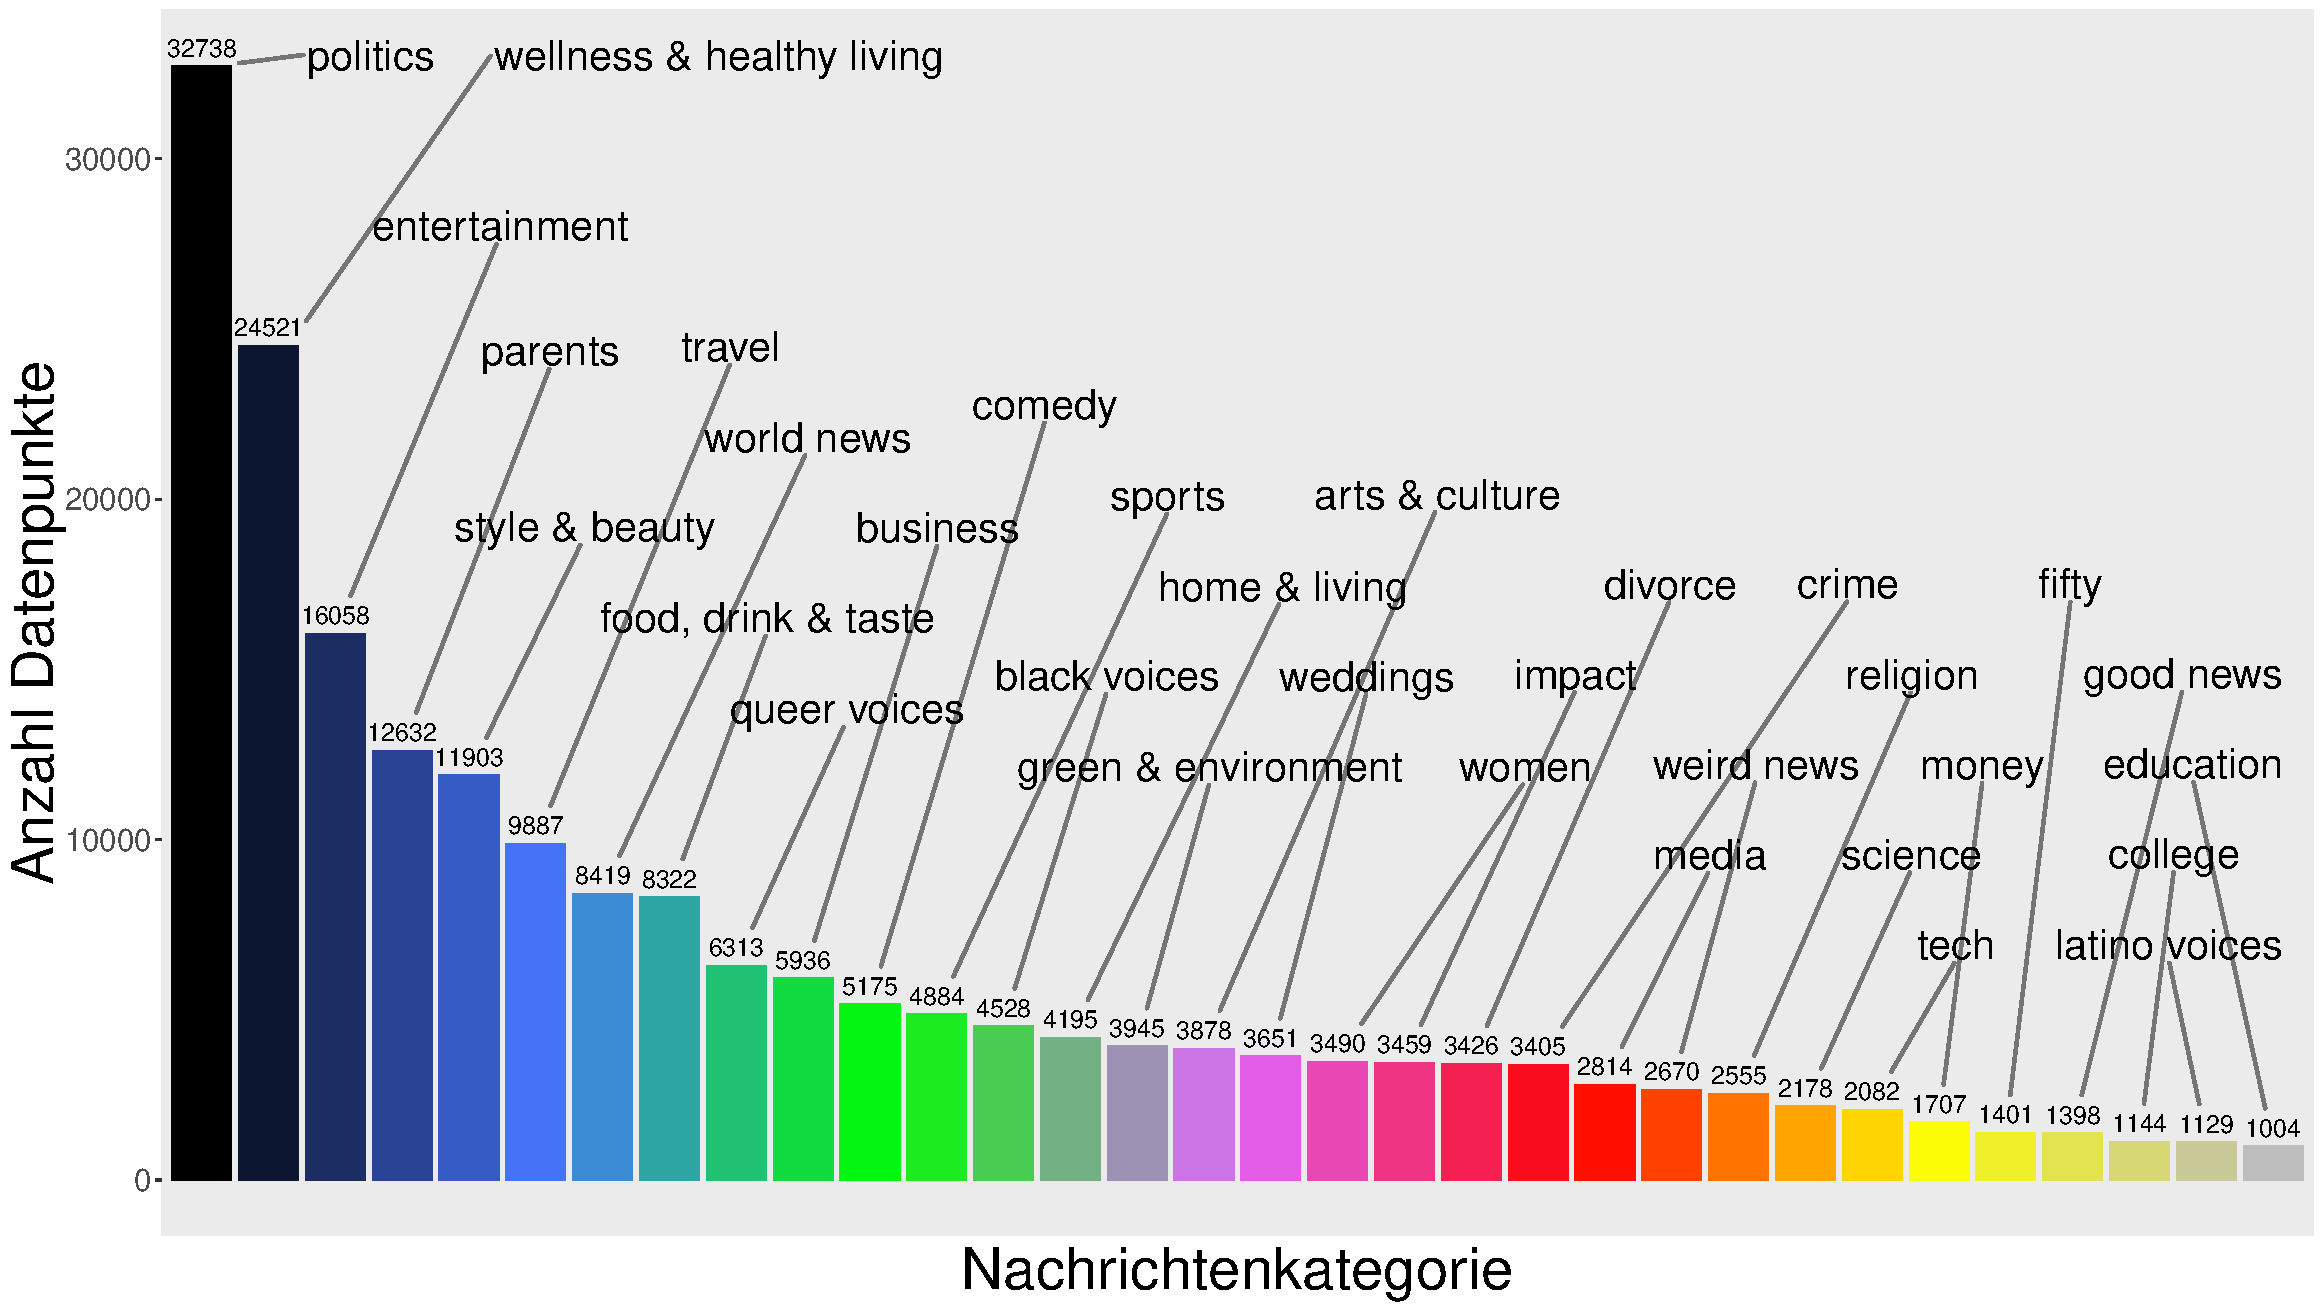
\includegraphics[width = \textwidth,  keepaspectratio]{Images/barplotCategories.pdf} 
\caption{Anzahl Datenpunkte pro Nachrichtenkategorie}
\label{abb:barplotCategories}
\end{figure}

Es ist festzustellen, dass die Kategorien keineswegs ausgeglichen vorliegen. Die häufigste Kategorie stellt \textit{politics} dar mit $\numprint{32738}$ Datenpunkten. Zweit- und dritthäufigste Kategorien sind \textit{wellness \& healthy living} und \textit{entertainment} mit $\numprint{24521}$ und $\numprint{16058}$ Beobachtungen. Die Nachrichtensparten mit den wenigsten Artikeln bilden \textit{college}, \textit{latino voices} und \textit{education} mit $\numprint{1144}$, $\numprint{1129}$ und $\numprint{1004}$ Beobachtungen.\\
Die ersten $6$ Kategorien stellen bereits $53.6$ Prozent der gesamten Beobachtungen dar. Durchschnittlich beinhaltet eine Kategorie $\numprint{6276.47}$ Nachrichtenschlagzeilen.\\
\\
Es folgt nun eine gesamtheitliche Exploration des Textkorpus der Schlagzeilen. Im Rahmen der Analyse zählen Symbole sämtlicher Art auch als Wörter. Die kürzeste Überschrift des Datensatzes enthält nur $1$ Wort, während die längste $82$ Wörter umfasst. Durchschnittlich enthält eine Artikel-Schlagzeile $11.022$ Wörter. Das Vokabular aller Schlagzeilen umfasst $\numprint{58717}$ Wörter, wobei \say{the} das häufigste Wort ist und in $\numprint{54139}$ Artikelüberschriften vorkommt. $\numprint{24372}$ Wörter kommen nur einmal vor. In der Betrachtung der mittleren Wortanzahlen pro Kategorie fällt auf, dass diese differieren. Die Kategorie mit der höchsten durchschnittlichen Anzahl von $12.724$ Wörtern ist \textit{style \& beauty}. Die Kategorie, bei der sich die Autoren durchschnittlich am kürzesten fassen, ist \textit{wellness \& healthy living} mit $9.367$ Wörtern. Eine weitere interessante Fragestellung ist, ob in den Kategorien bestimmte Sonderzeichen oder Symbole besonders häufig oder selten vorkommen. Abbildung \ref{abb:barplotSymbols} zeigt die relative Anzahl der Vorkommnisse verschiedener Symbole in den Schlagzeilen pro Kategorie.

\begin{figure}[ht]
    \centering
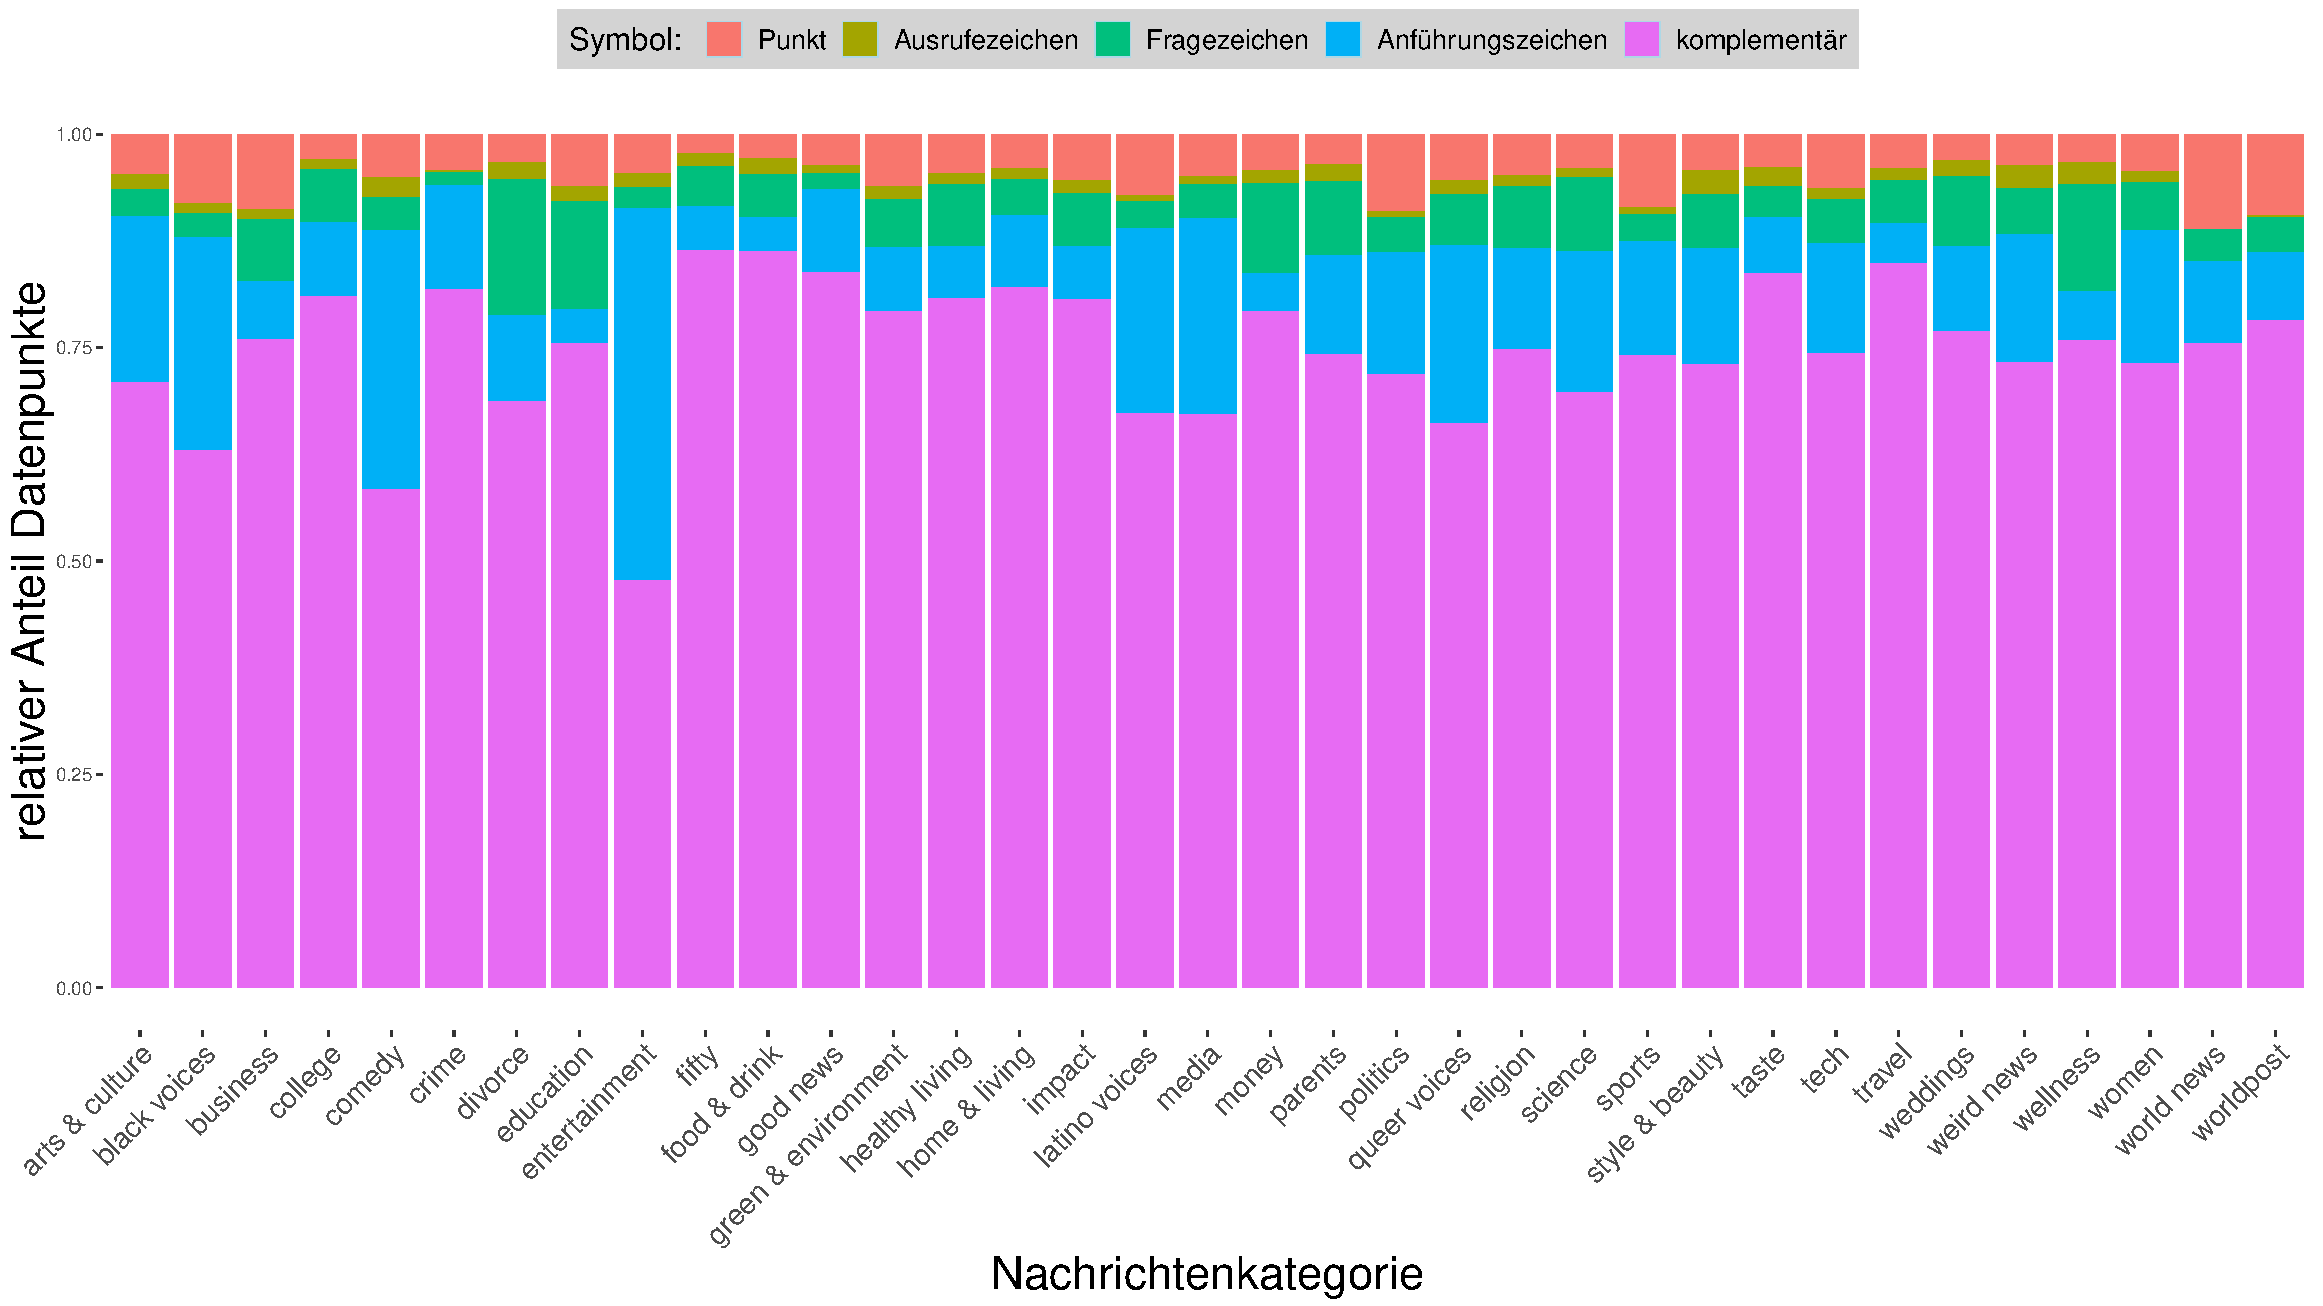
\includegraphics[width = \textwidth,  keepaspectratio]{Images/barplotSymbols.pdf} 
\caption{Relativer Anteil Datenpunkte für ausgewählte Sonderzeichen pro Kategorie. Der komplementäre Anteil ist der Anteil Datenpunkte, in dem keine der aufgeführten Sonderzeichen enthalten sind.}
\label{abb:barplotSymbols}
\end{figure}

Ein Wert von beispielsweise $0.15$ für eine bestimmte Nachrichtensparte in der Grafik ist so zu interpretieren, dass in $15$ Prozent aller Schlagzeilen dieser Kategorie das entsprechende Symbol mindestens einmal aufgetaucht ist. Die im Folgenden beschriebenen Durchschnitte sind Mittelwerte pro Kategorie und werden nicht über den gesamten Datensatz berechnet. Betrachtet sei nun das Vorkommen eines Punktes in einer Schlagzeile. Dieses kann so interpretiert werden, dass eine Schlagzeile mehrere Sätze enthält. Dies ist insgesamt mit einem durchschnittlichen relativen Anteil von $0.050$ selten der Fall. In der Sparte \textit{world news} kommen mehrere Sätze mit $0.098$ am häufigsten vor, in \textit{fifty} mit $0.021$ am wenigsten. Der Mittelwert für Ausrufezeichen beträgt $0.015$ und die Kategorie \textit{style \& beauty} nimmt das Maximum mit $0.028$, die Kategorie \textit{world news} das Minimum mit $0.002$ an. Fragezeichen kommen in durchschnittlich $0.059$ der Schlagzeilen vor, dabei am häufigsten in \textit{divorce} mit $0.159$ und am seltensten mit $0.015$ in \textit{crime}. Anführungszeichen sind mit durchschnittlich $0.133$ von den hier betrachteten Satzzeichen am meisten vertreten. Sie wurden besonders oft mit $0.437$ in der \textit{entertainment} Sparte genutzt und kamen am seltensten mit $0.040$ in \textit{education} zum Einsatz. Die Rubrik \say{komplementär} gibt an, zu welchem relativen Anteil keines der betrachteten Symbole vorkommt. Durchschnittlich enthalten $0.743$ der Kategorien keine der hier betrachteten Sonderzeichen. Hier ist zu sehen, dass Kategorien wie \textit{entertainment}, \textit{comedy}, \textit{black voices} oder \textit{divorce} häufig Symbole beinhalten, die einen dramatischen Charakter ausdrücken. Sparten wie \textit{fifty}, \textit{food, drink \& taste} und \textit{travel} bleiben mit wenig Symbolen sachlicher. Abbildung \ref{abb:barplotSymbols} zeigt insgesamt, dass Symbole für die Kategorisierung der Nachrichtensparten wichtig sind und im Rahmen der in Kapitel \ref{Kap:Tfidf} beschriebenen \textit{bag-of-words} und \textit{tf-idf}  Methoden nicht entfernt werden sollten.

\begin{figure}[ht]
    \centering
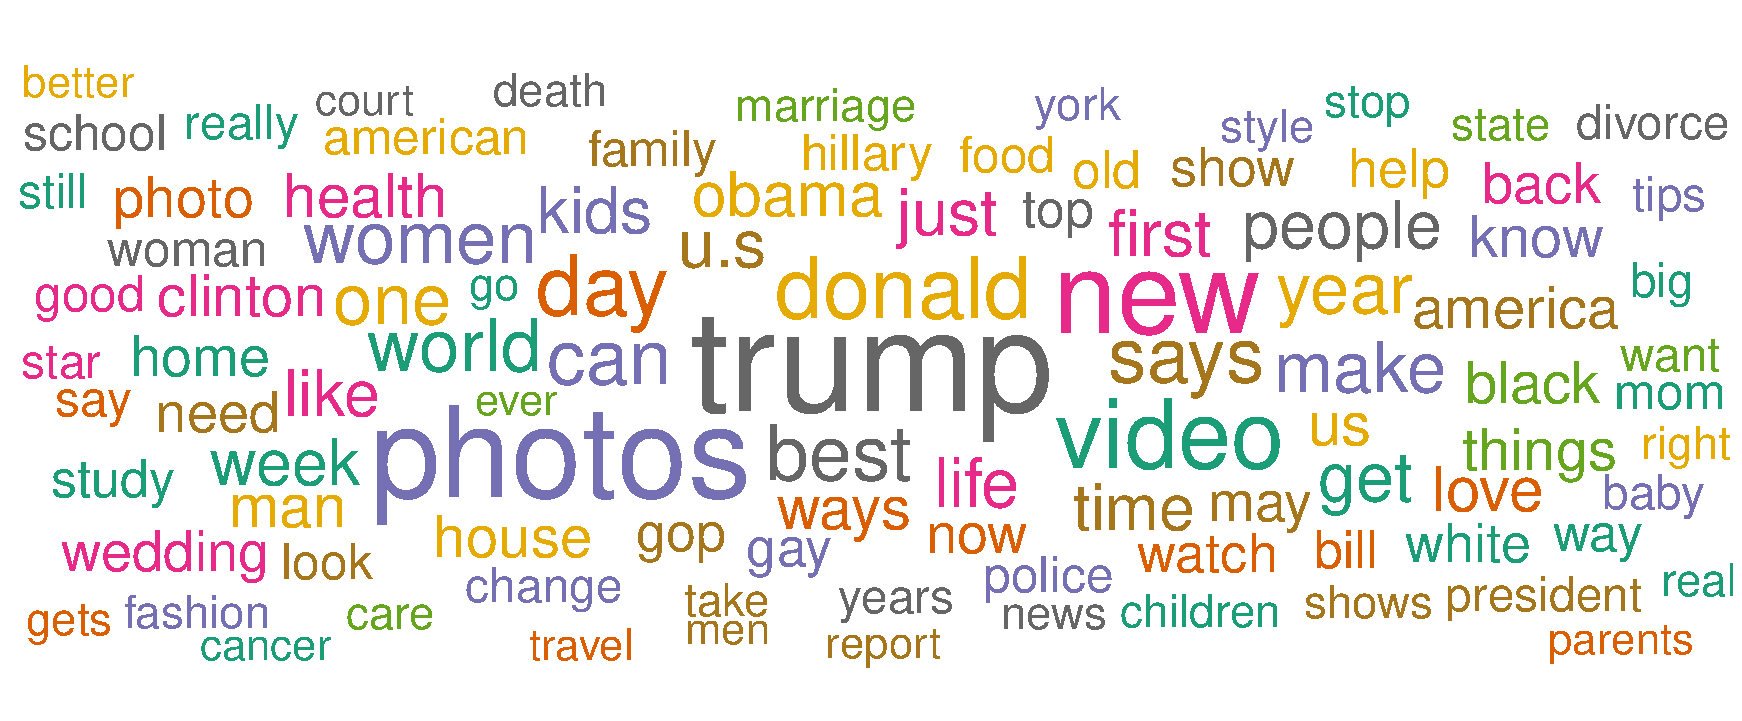
\includegraphics[width = \textwidth,  keepaspectratio]{Images/wordCloudAll.pdf} 
\caption{\textit{wordcloud} für die häufigsten 100 Wörter aller Kategorien}
\label{abb:WordcloudAll}
\end{figure}
todo: grafik gescheit ausfüllen

Je größer ein Wort, desto häufiger kommt es insgesamt im Textkorpus vor. Es ist erstaunlich, dass \say{trump} sich über den gesamten Textkorpus als häufigstes Wort etabliert hat, in Anbetracht dessen, dass sich der Zeitraum der Daten auf über $6$ Jahre erstreckt. Die $3$ häufigsten Wörter danach sind \say{photos}, \say{new} und \say{video}. Das überraschend sehr häufige Vorkommen der Wörter \say{photos} und \say{video} könnte ein Indiz dafür sein, dass in einigen Schlagzeilen bereits die Quelle des Medienmaterials angegeben ist, das im Artikel erscheint. Es ist zu sehen, dass viele Namen und Begriffe aus der Politik zu sehen sind, was einleuchtend ist, da \textit{politics} die größte Sparte darstellt. 
Auffallend ist außerdem, dass viele der auftauchenden Begriffe identisch oder fast identisch zu den Namen einiger Kategorien sind. Beispiele dafür sind \say{travel}, \say{wedding}, \say{style} oder \say{parents}. In Abbildung \ref{abb:WordcloudWellness} ist eine weitere \textit{Wordcloud} der zweitgrößten Sparte \textit{wellness \& healthy living} zu sehen.

\begin{figure}[ht]
    \centering
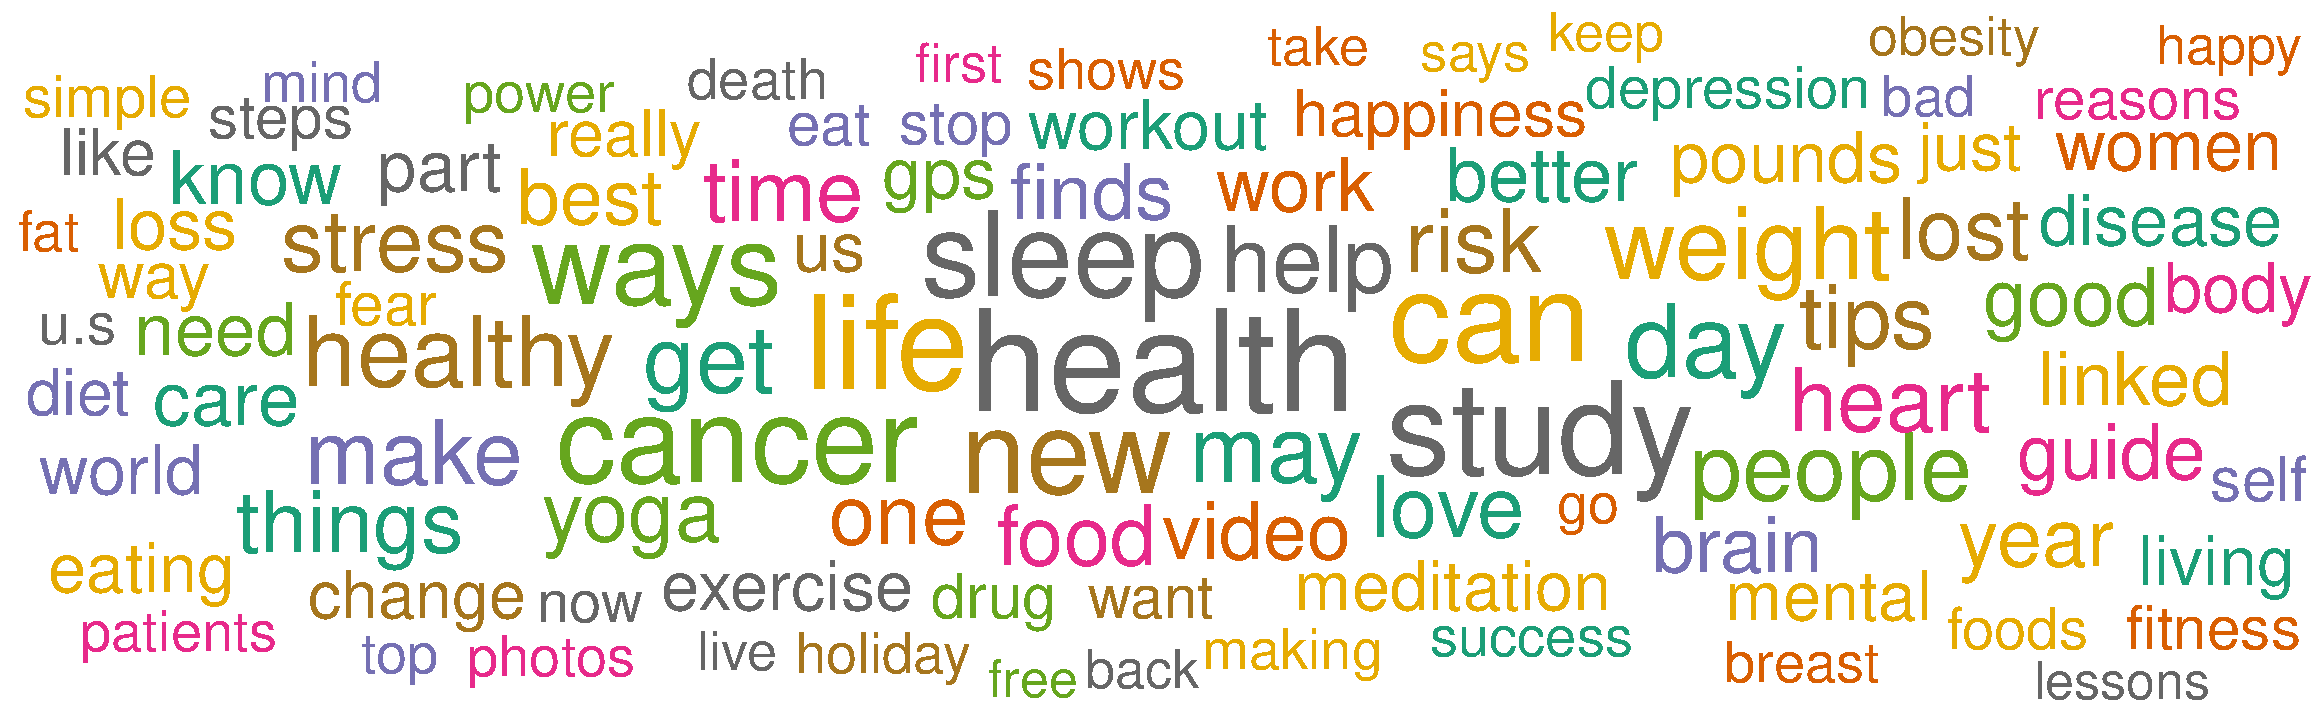
\includegraphics[width = \textwidth,  keepaspectratio]{Images/wordCloudWellness.pdf} 
\caption{\textit{Wordcloud} für die häufigsten 100 Wörter der Kategorie \textit{wellness \& healthy living}}
\label{abb:WordcloudWellness}
\end{figure}

In dieser Kategorie ist zu beobachten, dass oft über Schlaf, Yoga, Meditation und Sport geschrieben wird. Es werden aber auch Krankheiten wie Krebs (\say{cancer}), Übergewichtigkeit (\say{obesity}) und Diabetis angesprochen. \say{yoga}, \say{breast}, \say{diet} oder \say{pounds} könnten auch legitime Schlagwörter für die \say{women} Sparte sein. Genauso ist zu vermuten, dass die Wörter \say{eat}, \say{foods} und \say{healthy} ebenso in \say{food, drink \& taste} oft vorzufinden sind. Mit dem Blick auf die \textit{wordclouds} und auch in Anbetracht der Zusammenlegung der Kategorien in Kapitel \ref{kap:2_2Aend} fällt auf, dass es nicht immer einfach ist, die Kategorien nur über ihre häufigsten Schlagwörter auseinanderzuhalten. Auf die verschiedenen Möglichkeiten, wie die Schlagzeilen in ein numerisches Datenformat überführt werden können, wird in Kapitel \ref{kap:3.1Wordemb} detailiert eingegangen.
Nachdem nun der Datensatz ausführlich exploriert wurde, folgt im nächsten Unterabschnitt die Zielstellung dieser Thesis.


\subsection{Zielstellung} \label{Kap:Zielst}

Für die Onlinezeitung \textit{Huffpost} kann es von Interesse sein, die Nachrichtensparte eines Artikels unter Vorlage der Schlagzeile automatisch zu kategorisieren. Neben der Kosten- und Zeiteinsparung würden so würden Fehleinschätzungen von Autoren in Form von unpassenden Kategorien vermieden werden.\\
In dieser Thesis wird demnach ein \textit{multiclass}-Klassifikations\-problem behandelt. Dabei ist die Zielvariable die Nachrichtenkategorie. Diese enthält $32$ Klassen und liegt als Text in kategorieller Form vor. Die in die Modellierung eingehende unabhängige Variable ist die Schlagzeile, welche als numerischer Vektor mit einer der Methoden aus Kapitel \ref{kap:3.1Wordemb} repräsentiert wird. In dieser Problemstellung ist jede Beobachtung genau einer Klasse zugehörig. 

Ziel dieser Arbeit ist es, im Rahmen dieses Klassifikationsproblems verschiedene Algorithmen auf verschiedenen Arten der Repräsentation der Wörter miteinander zu vergleichen. 

Sei $\bm{x}_i$ die Repräsentation der $i$-ten Beobachtung als Vektor und $y_i \in \{c_1, ..., c_{32} \}$ die zugehörige Klasse. Die Klassen $\{c_1, ..., c_{32} \}$ können als natürliche Zahlen $\{1, ..., 32 \}$ dargestellt werden.
%(todo checken)
%, oder als Vektoren $\bm{c}_j \in \mathbb{R}^{32}, j %\in \{1,...,32\}$, wobei sie an der $j$-ten Stelle %eine $1$ enthalten und $0$ sonst.


Für die Vorhersagen $f(\bm{x}_i)$ der trainierten Modelle gilt dann, dass
\begin{center}
$f(\bm{x}_i) = \bm{p}_i = (p(c_1), ...., p(c_{32}))_i$, \hspace{2cm} mit $\sum\limits_{i = 1}^{32} p(c_i) = 1 $,
\end{center}
dabei sind $p(c_j)$, $j = 1,...,32$ die modellierten Wahrscheinlichkeiten der Zugehörigkeit der Beobachtung $\bm{x_i}$ zur Klasse $c_j$, die in Summe $1$ ergeben müssen. Die eindeutige prognostizierte Klasse $\hat{y}_i$ wird dann zugeordnet durch 
\begin{center}
    $\hat{y_i} =  \underset{c_1,...,c_{32}}{argmax}$ $p(c_j)$.
\end{center}

Zur Messung der Performance der Modelle erfolgt anhand der Gütemaße aus Kapitel \ref{kap:guetemass} ein Vergleich. Dabei ist nicht nur von Interesse, wie gut die Modelle insgesamt abschneiden, sondern auch ob manche Modelle bestimmte Kategorien trennschärfer identifizieren können und welche Gründe es dafür gibt. Des Weiteren soll analysiert werden, in welche Nachbarklassen die Beobachtungen bei einer Fehlklassifikation eingeordnet werden und ob diese inhaltlich nahe an der richtigen Kategorie sind. Eine weitere Untersuchungsfrage für die Modellgüte ist, inwiefern die Repräsentation der Wörter ausschlaggebend ist und welches Gewicht der verwendete Algorithmus dabei einnimmt.
Nun sollen im nächsten Abschnitt die statistischen Methoden beschrieben werden.
(todo: diesen Abschnitt im Laufe der Arbeit ergänzen)

\newpage


\section{Statistische Methoden}

Dieses Kapitel ist in $3$ Abschnitte unterteilt. Zuerst werden die zur Bewertung der Modelle herangezogenen Gütemaße beschrieben. Es folgt die Darlegung der verschiedenen Methoden zur numerischen Repräsentation von Wörtern. Zuletzt folgt die ausführliche Beschreibung der in dieser Arbeit benutzten \textit{Machine-Learning} Algorithmen.

\subsection{Gütemaße zur Evaluation der Modelle}\label{kap:guetemass}

Die Bewertung der Modelle erfolgt über verschiedene Kennzahlen. Einige davon werden unter Verwendung der \textit{Confusion Matrix} (oder auch Klassifikationsmatrix) berechnet. Wird das Modell auf die Testdaten angewandt und für jeden Datenpunkt eine Kategorie vorhergesagt, so stellt die in Tabelle \ref{tab:confusionMatrix} abgebildete Matrix die resultierenden Richtig- und Fehlklassifikationen für $C$ Klassen dar.

\begin{table}[ht]
\begin{center}
\begin{tabular}{|c|ccc|c|}
  \hline
 & \multicolumn{3}{|c|}{Prognostizierte Klasse} &  \\
Wahre Klasse & Kategorie $c_1$ & ...  & Kategorie $c_C$ & Zeilensumme  \\ 
  \hline
Kategorie $c_1$ & $h_{11}$ & $\hdots$ & $h_{1C}$ & $\sum_{j=1}^C h_{1j}$\\
$\vdots$ & $\vdots$ & $\ddots$ & $\vdots$ & $\vdots$ \\
Kategorie $c_C$ & $h_{C1}$ & $\hdots$ & $h_{CC}$ & $\sum_{j=1}^C h_{Cj}$\\
\hline
Spaltensumme & $\sum_{i=1}^C h_{i1}$ & $\vdots$ & $\sum_{i=1}^C h_{iC}$ & 
$N = \sum_{i=1}^C \sum_{j=1}^C h_{ij}$\\
   \hline
\end{tabular}

  \caption{Übersicht über eine \textit{Confusion Matrix}  für $C$  Klassen (vgl. \cite{backhaus}, S. 238)}  
  \label{tab:confusionMatrix}
\end{center}
\end{table}

Die absoluten Häufigkeiten $h_{ij}$ stehen für die Anzahl der Beobachtungen aus der wahren Klasse $i$, für die die Klasse $j$ prognostiziert wurde. Summiert man alle Einträge der Matrix, so erhält man die Anzahl der Beobachtungen $N$. Aus der \textit{Confusion Matrix} können folgende Größen identifiziert werden: Die \textit{True-Positives} der Klasse $i$, $tp_i = h_{ii}$ sind alle Beobachtungen, die Klasse $i$ zugehörig sind und auch in selbige klassifiziert wurden. Die Beobachtungen, die in Klasse $i$ klassifiziert wurden, aber einer anderen wahren Klasse zugehörig sind, bezeichnet man als \textit{False-Positives} $fp_i = \sum_{j = 1}^C h_{ji} - h_{ii}$. Als \textit{False-Negatives} $tn_i = \sum_{j = 1}^C h_{ij} - h_{ii}$ werden die Beobachtungen bezeichnet, die der Klasse $i$ zugehörig sind, aber in eine andere Kategorie falsch klassifiziert werden. Letztlich sind \textit{True-Negatives} $tn_i = N - (fp_i + tn_i + tp_i)$ die Datenpunkte, die nicht Kategorie $i$ angehören und für die auch nicht Klasse $i$ prognostiziert wird (vgl. \cite{sokolova}, S. 3). Unter Kenntnis der $4$ Häufigkeiten können nun verschiedene Gütemaße berechnet werden. 


Die \textit{Accuracy} berechnet sich analog zur binären Klassifikation aus 
\[ Accuracy = \frac{\sum_{i=1}^C tp_i}{N},  \]
ist also der Anteil der richtig klassifizierten Beobachtungen an allen Beobachtungen. Dieses Maß ist jedoch gerade bei unbalancierten Klassifikationsproblemen nicht ideal, da große Klassen stark favorisiert werden und ein Modell schon eine hohe Güte erzielen kann, indem es alle Beobachtungen der größten Klasse zuordnet (vgl. \cite{backhaus}, S.239). Es folgen die Maße \textit{Precision}, \textit{Recall} und darauf aufbauende Kennzahlen, welche bei unterschiedlichen Klassengrößen geeigneter sind. Es wird von einer hohen \textit{Precision} der Klasse $i$ gesprochen, wenn nach Prognose in Klasse $i$ ein hoher Anteil dieser Beobachtungen auch tatsächlich aus derselben Kategorie stammt. Wiederum hat das Modell bezüglich Klasse $i$ einen hohen \textit{Recall}, falls von den Beobachtungen der wahren Klasse $i$ auch ein hoher Anteil in Klasse $i$ eingeordnet wird.
In der \textit{Multiclass}-Klassifikation kann ein Gütemaß für das komplette Modell über \textit{Micro-Averaging} (mit $\mu$ indiziert) oder \textit{Macro-Averaging} (mit $M$ indiziert) über alle Klassen berechnet werden. Es sind dann 
\[ Precision_{\mu} = \frac{\sum_{i = 1}^C tp_i}{\sum_{i = 1}^C (tp_i + fp_i)}, \hspace{1cm} Recall_{\mu} = \frac{\sum_{i = 1}^C tp_i}{\sum_{i = 1}^C (tp_i + fn_i)},\]
\[ Precision_M = \frac{\sum_{i = 1}^C \frac{tp_i}{tp_i + fp_i} }{C}, \hspace{1cm} Recall_M = \frac{\sum_{i = 1}^C \frac{tp_i}{tp_i + fn_i} }{C}\]
die Gütemaße für das gesamte Modell. Ein Maß, dass \textit{Precision} und \textit{Recall} kombiniert ist der \textit{fscore}. Mit der unterschiedlichen Durchschnittsbildung ergeben sich
\[ fscore_{\mu}^{(\beta)} = \frac{(\beta^2+1) \cdot Precision_{\mu} \cdot Recall_{\mu}}{\beta^2 Precision_{\mu}+ Recall_{\mu}}, \hspace{1cm} fscore_{M}^{(\beta)} = \frac{(\beta^2+1) \cdot Precision_{M} \cdot Recall_{M}}{\beta^2 Precision_{M}+ Recall_{M}} . \]

todo: $\overline{Accuracy} = \frac{1}{C} \sum_{i = 1}^C Accuracy_{C_i}$\\
$\bar{p}_{IfCorrect} = \frac{1}{N}\sum_{i=1}^N  I_{\{\hat{y}(x_i) = y_i\}} p(x_i = y_i)$\\


Hierbei ist anzumerken, dass $fscore_{\mu}^{(\beta)}$ Klassen mit vielen Beobachtungen in der Güte begünstigt während für $fscore_M^{(\beta)}$ alle Kategorien gleich wichtig sind  (vgl. \cite{sokolova}, S.3ff). Der Parameter $\beta$ gibt in den Formeln an, was für ein Gewicht \textit{Recall} im Verhältnis zu \textit{Precision} einnimmt.
Wie bei dem \textit{f1-score} Maß einer binären Klassifikation wird in dieser Arbeit $\beta = 1$ verwendet. \textit{Recall} und \textit{Precision} besitzen also identische Wichtigkeit. \\
Bei Betrachtung des Nenners in der Berechnung von $Precision_{\mu}$ und $Recall_{\mu}$ fällt auf, dass in beiden Fällen durch die gesamte Summe der \textit{Confusion Matrix} geteilt wird. Diese Summe entspricht dem Nenner $N$ bei der Berechnung der $Accuracy$. Ist nun auch $\beta = 1$, so gilt 
\[Precision_{\mu} =  Recall_{\mu} =  fscore_{\mu}^{(1)} = Accuracy.\]

Für eine beispielhafte Erklärung dieses Sachverhaltes sei auf \cite{towards1}
%todo: shmueli (2019) verwiesen
verwiesen. Aus diesem Grund wird statt der mit \textit{Micro-Averaging} berechneten Gütemaße in der statistischen Auswertung in Kapitel \ref{Kap:statAus} die $Accuracy$ verwendet.\\

Ein weiteres Maß, um die Güte eines Multiklassifikationsproblems zu bewerten, ist die gemittelte \textit{Categorical Cross Entropy} (kurz \textit{CE}). Diese berechnet sich aus

\[ CE = - \frac{1}{N}\sum_{i=1}^N \sum_{j = 1}^C y_{ij} log(p_i(c_j)) \hspace{2cm} y_{ij} \in \{0,1\} \hspace{0.2cm} \forall i, j = 1,...,N \hspace{0.2cm} ,\]

wobei $y_{ij}$ indiziert, ob die Beobachtung $i$ der wahren Klasse $j$ zugehörig ist. $p_i(c_j)$ gibt die vom Modell modellierte Wahrscheinlichkeit an, dass Beobachtung $i$ zu Klasse $j$ gehört (vgl. \cite{murphy}, S.571). Da $y_{ij}$ immer $0$ für alle falsch vorhergesagten Klassen ist, entspricht $CE$ dem negativen Mittelwert der logarithmierten Wahrscheinlichkeiten der wahren Klassen über alle Beobachtungen. So wird eine geschätzte Wahrscheinlichkeit nahe $0$ für die wahre Klasse stark bestraft und eine hohe Wahrscheinlichkeit trotz einer Fehlklassifikation weniger bestraft. Je sicherer sich das Modell für die wahren Kategorien ist, desto niedrigere Werte wird dieses Gütemaß annehmen (vgl. \cite{proMachine}, S. 72). 
Dabei gilt es die \textit{Cross Entropy} zu minimieren. Sie nimmt ihr Minimum bei $0$ im Idealfall an, wenn für alle Beobachtungen eine Wahrscheinlichkeit von $1$ für die wahre Klasse prognostiziert wird. Die $CE$ wird oft als Verlustfunktion für die Modellanpassung auf den Trainingsdaten verwendet, wie zum Beispiel bei dem \textit{XGBoost}-Algorithmus und den \textit{Deep Learning} Verfahren aus Kapitel \ref{kap:neuralNets}.\\
\\
Die in diesem Abschnitt beschriebenen Maße können sowohl auf den Trainingsdaten als auch auf den  Validierungs- und Testdaten berechnet werden. Ein Vergleich der Modelle in der Vorauswahl in Abschnitt \ref{kap:preselection} erfolgt über die Evaluation auf den Validierungsdaten. Dabei werden die Maße $Accuracy$, $CE$, und $fscore_M^{(1)}$ genutzt.
Bei dem Vergleich der finalen Modelle in Kapitel \ref{kap:evalFinal} erfolgt die Auswertung der Performanzmaße auf den ungesehenen Testdaten. (todo: aufführen was noch alles verwendet wurde).


\subsection{Methoden zur numerischen Repräsentation der Wörter} \label{kap:3.1Wordemb}

Das Extrahieren von Informationen aus Texten ist keine triviale Aufgabe, für die es viele Methoden gibt. In diesem Abschnitt werden einige Methoden aufgezählt, die in dieser Thesis zum Einsatz kommen.
Die beschriebenen Repräsentationen der Wörter werden folglich auch als \textit{Embeddings} oder \textit{Word-Embeddings} bezeichnet.


\subsubsection{\textit{Bag-Of-Words} und \textit{Term Frequency Inverse Document Frequency}} \label{Kap:Tfidf}

Bei diesen Methoden wird zuerst für den gesamten Textkorpus ein Vokabular gebildet, das für jedes vorkommende Wort die absolute Häufigkeit des Vorkommens sowie die Anzahl der Dokumente (ein Dokument ist ein Datenpunkt, also eine Schlagzeile) enthält, in der das Wort vorkommt. Aus diesem Vokabular wird anschließend die \textit{Document-Term-Matrix} (kurz \textit{DTM}) geformt, die für jede der $N$ Beobachtungen eine Zeile und für jede der $V$ Wörter im Vokabular eine Spalte enthält. Eine beispielhafte \textit{DTM} für ist in Tabelle dargestellt.

\begin{table}[ht]
\begin{center}
    

\begin{tabular}{|c||ccccccccccc|}
\hline
\multicolumn{12}{|c|}{\textit{BOW} \textit{DTM}} \\
\hline 
   Satz   & the & dog & cat & like & likes &  to & sit  & owner & his &  does & not \\
      \hline
Satz 1 & $1$ & $0$ & $1$ & $0$ & $1$ & $1$ & $1$ & $0$ & $0$ &  $0$ & $0$ \\
Satz 2 & $1$ & $1$ & $0$ & $1$ & $0$ & $0$ & $0$ & $1$ & $1$ &  $1$ & $1$ \\
Satz 3 & $1$ & $1$ & $0$ & $0$ & $1$ & $0$ & $0$ & $1$ & $0$ &  $0$ & $0$ \\

\hline

\multicolumn{12}{|c|}{\textit{TFIDF} \textit{DTM}} \\
\hline 
   Satz   & the & dog & cat & like & likes &  to & sit  & owner & his &  does & not \\
      \hline
Satz 1 & $0.243$ & $0$ & $0.398$ & $0$ & $0.301$ & $0.398$ & $0.398$ & $0$ & $0$ &  $0$ & $0$ \\
Satz 2 & $0.243$ & $0.301$ & $0$ & $0.398$ & $0$ & $0$ & $0$ & $0.301$ & $0.398$ &  $0.398$ & $0.398$ \\
Satz 3 & $0.243$ & $0.226$ & $0$ & $0$ & $0.226$ & $0$ & $0$ & $0.226$ & $0$ & $0$ & $0$ \\
\hline
\end{tabular}
\end{center}{}
\caption{Beispiel für eine \textit{Document-Term-Matrix} für die $3$ Beispielsätze \textit{the cat likes to sit}, \textit{the dog does not like his owner}, \textit{the owner likes the dog} jeweils für das \textit{BOW Embedding} und das \textit{TFIDF Embedding} }  
\label{tab:BOWExample}

\end{table}

Der Textkorpus im oben stehenden Beispiel besteht aus insgesamt $11$ Wörtern und jede der Spalten der Matrix repräsentiert eines davon.
Die Einträge der \textit{DTM} bestehen aus Werten, die das Aufkommen der Wörter beschreiben. Im simplen \textit{Bag-Of-Words} Ansatz (kurz: \textit{BOW}) ist $dtm_{ij} = f_{d_i t_j}$ die Anzahl von Wort $t_j$ in Dokument $d_i$ (vgl. \cite{deepEssentials} S. 117f). Dies ist im oberen Teil von Tabelle \ref{tab:BOWExample} veranschaulicht. Es gibt einige Wörter wie \textit{the} oder \textit{and}, die häufig vorkommen aber eventuell nicht wichtig sind. Diese \textit{stopwords} können für die \textit{BOW} Methode entfernt werden. Dies muss aber nicht erfolgen, da manche \textit{stopwords} in einigen Kategorien häufiger vorkommen können als in anderen. Für das Beispiel in Tabelle \ref{tab:BOWExample} wurden die \textit{stopwords} nicht entfernt.
Bei einem \textit{BOW Embedding} wird nur gezählt, wie oft ein Wort absolut vorkommt, dabei wird aber nicht berücksichtigt, dass manche Wörter in einigen Dokumenten eine höhere Bedeutung haben können als in anderen. \\

Ein Ansatz, der diese Problematik berücksichtigt ist \textit{Term Frequency Inverse Document Frequency} (kurz: \textit{TFIDF}). Hierbei werden die Einträge $dtm_{ij}$ bei häufig benutzten Ausdrücken verringert und erhöht für Wörter, die insgesamt selten benutzt werden (vlg. \cite{textMiningR} S.29). Die \textit{TFIDF} für das Dokument $d_i$ und das Wort $t_j$ berechnet sich aus 
\[TFIDF(d_i, t_j) = TF(d_i,t_j) \cdot IDF(t_j) . \]
Sowohl für die \textit{Term-Frequency} $tf$ als auch für die \textit{Inverse-Document-Frequency} $idf$ gibt es verschiedene Möglichkeiten zur Berechnung, wobei in dieser Thesis folgende Formeln genutzt werden.
Die \textit{Augmented-Term-Frequency}

\[TF(d_i,t_j) = 0.5 +  0.5 \cdot \frac{f_{d_i t_j}}{max \{ f_{d_i t_j'}: t_j' \in d_i \}} \].

berücksichtigt eine Verzerrung bei längeren Dokumenten, indem durch das Maximum der Häufigkeiten der vorkommenden Wörter in dem Dokument dividiert wird. Der Summand $0.5$ und der Multiplikator $0.5$ dienen der Normalisierung. Für die \textit{Inverse-Document-Frequency} ist der Quotient zwischen der Anzahl der Dokumente $N$ im Korpus und der Anzahl der Dokumente, die das Wort enthalten, ein geeignetes Maß (vgl. \cite{deepEssentials} S. 118):

\[IDF(t_j) = log \Bigl( \frac{N}{\# \{d_i: t_j \in d_i \}} \Bigr) .\]

In dem unteren Teil von Tabelle \ref{tab:BOWExample} ist die resultierende \textit{DTM} unter Nutzung des beschriebenen \textit{TFIDF Embeddings} dargestellt. Es ist zu sehen, dass nur einmal im Textkorpus vorkommende Wörter (\say{\textit{his}}), ein höheres Gewicht bekommen als Wörter, die oft vorkommen (\say{\textit{the}}). Zudem kann das gleiche Wort ein unterschiedliches Gewicht in verschiedenen Datenpunkten enthalten (\say{\textit{dog}}).

Die Umsetzung im Programmiercode erfolgte mit dem \texttt{R}-Paket \texttt{text2vec} (\cite{text2vec}).

Unter Nutzung von sowohl \textit{BOW} als auch \textit{TFIDF} für die Repräsentation von Wörtern wird die Reihenfolge in den Dokumenten vernachlässigt (vgl. \cite{deepEssentials} S. 117). 
Die nachfolgend beschriebenen Methoden berücksichtigen hingegen die Reihenfolge der Wörter in einem Satz.


\subsubsection{\textit{GloVe: Global vectors for representation of words}} \label{Kap:Glove}

Eine weitere Methode zur numerischen Repräsentation von Texten sind \textit{Word Embeddings}, bei denen Wörter zu Vektoren fester Länge mit numerischen Werten kodiert werden. Mittlerweile haben sich \textit{Word Embeddings} als präferierte Methode für alle Bereiche der Sprachverarbeitung im \textit{Machine-Learning} durchgesetzt. Die beiden bekanntesten Methoden um \textit{Word Embeddings} zu generieren sind \textit{Word2vec} und \textit{GloVe} (vgl. \cite{keras}, S. 139). Obwohl \textit{Word2vec} auf dem Lernen durch ein neuronales Netz basiert und \textit{GloVe} auf der Zählung des Vorkommens von Wörtern im Kontext aufbaut, sind die beiden Verfahren von der grundsätzlichen Herangehensweise und den Resultaten ähnlich. Beide Methoden konstruieren einen Vektorraum, in dem die Position eines Worts durch den Kontext bestimmt wird, in dem das Wort im Textkorpus auftritt.
\textit{GloVe} liefert im Vergleich zu \textit{Word2vec} generell etwas bessere Resultate und ist mit Parallelisierung schneller zu berechnen (vgl. \cite{keras}, S. 156). Aus diesen Gründen wird in dieser Thesis \textit{GloVe} verwendet und im Folgenden beschrieben. \\
Die Methode nutzt ein unüberwachtes Lernen zur Konstruktion der Vektoren. Zuerst wird eine \textit{Term-Co-Occurance} (kurz \textit{TCM}) Matrix $R$ konstruiert, die so viele Zeilen enthält, wie das Vokabular Wörter besitzt. Die Spalten stehen auch für die Wörter des Vokabulars, allerdings als Kontext verstanden. Tabelle \ref{tab:GloveExample} verdeutlicht dies anhand des Beispiels aus Tabelle \ref{tab:BOWExample}.

\begin{table}[ht]
\begin{center}
  
 \begin{tabular}{|l||ccccccccccc|}
  \hline
  & \multicolumn{11}{|c|}{Kontext} \\
\hline 
Wörter & the & dog & cat & like & likes & to & sit & owner & his & does & not \\ 
  \hline
the & 0 & 0 & 0 & 0 & 0 & 0 & 0 & 0 & 0 & 0 & 0 \\ 
  dog & 2  & 0  & 0  & 0  & 1 & 0 & 0 & 0 & 0 & 0 & 0 \\ 
  cat & 1 & 0 & 0 & 0 & 1 & 1 & 0 & 0 & 0 & 0 & 0 \\ 
  like & 0 & 0 & 0 & 0 & 0 & 0 & 0 & 1 & 0 & 0 & 1 \\ 
  likes & 3 & 0 & 0 & 0 & 0 & 0 & 0 & 0 & 0 & 0 & 0 \\ 
  to & 0 & 0 & 0 & 0 & 1 & 0 & 0 & 0 & 0 & 0 & 0 \\ 
  sit & 0 & 0 & 0 & 0 & 1 & 1 & 0 & 0 & 0 & 0 & 0 \\ 
  owner & 2 & 0 & 0 & 0 & 1 & 0 & 0 & 0 & 0 & 0 & 0 \\ 
  his & 0 & 0 & 0 & 1 & 0 & 0 & 0 & 1 & 0 & 0 & 1 \\ 
  does & 1 & 1 & 0 & 1 & 0 & 0 & 0 & 0 & 0 & 0 & 1 \\ 
  not & 0 & 1 & 0 & 0 & 0 & 0 & 0 & 0 & 0 & 0 & 0 \\ 
   \hline
\end{tabular}  
 
\end{center}{}
\caption{Beispiel für eine \textit{Term-Co-Occurance} Matrix für die $3$ Beispielsätze \textit{the cat likes to sit} (Satz $1$), \textit{the dog does not like his owner} (Satz $2$), \textit{the owner likes the dog} (Satz $3$) für einen symmetrischen Fensterbereich von 2}  
\label{tab:GloveExample}

\end{table}

In den Einträgen der \textit{TCM} Matrix stehen nun die Häufigkeit des Vorkommens der Wörter (Zeilen) im jeweiligen Kontext (Spalten). Ob ein Wort im Kontext vorkommt, ist so zu verstehen, dass es in einem vom Anwender wählbaren Fensterbereich um das Kontextwort enthalten ist. So kommt für einen symmetrischen Bereich von $2$ in Tabelle \ref{tab:GloveExample} das Wort \say{likes} dreimal im Kontext von \say{the} vor, einmal in Satz $1$ und zweimal in Satz $3$. Obwohl \say{dog} und \say{owner} in Satz $2$ und Satz $3$ zusammen vorkommen, steht in der \textit{TCM} an der betreffenden Stelle eine $0$. Zur Berechnung der \textit{GloVe Embeddings} wird nun die \textit{TCM} Matrix $\bm{R}$ in das Produkt aus $2$ Matrizen $\bm{P}$ und $\bm{Q}$ zerlegt, die multipliziert eine Matrix $\bm{\Tilde{R}}$ ergeben:

\begin{equation*}
\underset{N \times N}{\bm{R}} = \underset{N \times F}{\bm{P}} \cdot \underset{F \times N}{\bm{Q}} \approx  \underset{N \times N}{\Tilde{\bm{R}}} 
\end{equation*}

Die Matrix $\bm{P}$ mit Dimension $N \times F$ ergibt multipliziert mit $\bm{Q}$ mit Dimensionen $F \times N$ wieder eine $N \times N$ Matrix. $F$ ist die Länge der resultierenden Wort-Vektoren und muss vom Anwender festgelegt werden. Diese Größe bestimmt den Raum $\mathbb{R^F}$, in dem die Wort-Vektoren die Wörter repräsentieren sollen. Nun werden zu Beginn sowohl $\bm{P}$ als auch $\bm{Q}$ mit zufälligen Werten initiiert und die Matrix $\bm{\Tilde{R}}$ berechnet. Mithilfe des stochastischen Gradienten-Abstiegs (mehr dazu in Kapitel \ref{kap:neuralNets}) wird nun der Inhalt von $\bm{P}$ und $\bm{Q}$ verändert, mit dem Ziel die Summe aller Einträge der Differenz von $\bm{\Tilde{R}}$ und $\bm{R}$ zu minimieren. Dies ist ein numerischer iterativer Prozess, der wiederholt wird, bis der Fehler eine vorgegebene untere Grenze erreicht und sich die Matrizen $\bm{\Tilde{R}}$ und $\bm{R}$ im Rahmen dieser Toleranz ähnlich sind. Die Matrix $\bm{P}$ enthält zeilenweise nun die gewünschten Wort-Vektoren für jedes der $N$ Wörter des Vokabulars (vgl. \cite{keras}, S. 155f). Für eine detailierte Beschreibung der Methode sei auf \cite{glovePaper} verwiesen. 
%todo: et al
Es ist möglich diese Vektoren auf dem vorliegenden Trainingsdatensatz zu trainieren, wenn der Textkorpus groß genug ist. In dem Fall des \textit{News Category Dataset} mit \numprint{200847} ist dies durchaus plausibel. Das Trainieren der Vektoren erfolgte mit dem \texttt{R}-Paket \texttt{text2vec} (\cite{text2vec}) unter Verwendung der Parameter $skip\_grams\_window = 5$ für den symmetrischen Bereich des Kontextworts und die Dimension der Vektoren von $F = 50$. Dieses \textit{Embedding} wird mit dem Kürzel \textit{GloVe unsup. 50D} referenziert. \\
Eine Alternative zum Training der \textit{Word-Embeddings} auf dem vorliegenden Textkorpus ist der Griff zu einem der vortrainierten Datensätze, die von \cite{gloveOnline}
%todo: o.D referenz?
zur Verfügung gestellt worden sind. Diese Vektoren wurden auf massiven Datenmengen trainiert. Für diese Arbeit wurden 2 Datensätze mit vor-trainierten Wortvektoren des \textit{GloVe} Projekts genutzt: Ein auf Wikipedia mit $6$ Milliarden Dokumenten trainierter Datensatz mit einer Länge der Vektoren von $F = 50$ (\cite{gloveWiki}) und ein auf $42$ Milliarden aus verschiedensten Quellen des Internets stammenden Textdokumenten mit $F = 300$ Dimensionen (\cite{gloveCommon}). Die beiden vortrainierten \textit{Embeddings} werden in Kapitel \ref{Kap:statAus} mit \textit{GloVe 50D} und \textit{GloVe 300D} referenziert.\\

Ob nun vor-trainierte \textit{Word Embeddings} genutzt werden oder die Vektoren auf dem Trainingsdatensatz gelernt werden, es stellt sich die Frage, wie genau die Datenpunkte geformt werden, sodass ein \textit{Machine-Learning} Modell immer Eingangswerte derselben Dimension erwarten kann. Nun ist unter der Annahme, dass eine Beobachtung immer aus einer Aneinanderreihung von Wörtern besteht, jeder durch Wort-Vektoren repräsentierter Datenpunkt $x_i$ bereits eine zweidimensionale Matrix mit Dimensionen $F \times  W_i$. $W_i$ steht für die Anzahl Wörter im Satz des Datenpunktes $x_i$ und $F$ ist die Anzahl der Wort-Vektoren. Die Trainingsdaten formen dann ein dreidimensionales Array $N \times F \times  W_i$, wobei $N$ die Anzahl der Datenpunkte im Trainingsset ist. In \texttt{R} müssen nun aber alle $N$ Matrizen die gleiche Anzahl Spalten und Zeilen besitzen, um zu einem Array geformt werden zu können.
Dementsprechend soll die Anzahl der Spalten $W_i$ immer gleich gewählt werden. Hier wird als Konstante $W_{max}$ die Anzahl Wörter gewählt, die $99.9$ Prozent der News Schlagzeilen im Trainingsset nicht überschreiten. Diese Konstante wird heuristisch vom Nutzer gewählt. Die verbleibenden längsten $0.1$ Prozent der Schlagzeilen werden entfernt.
Für jede Schlagzeile, die weniger Wörter als $W_{max}$ enthält, wird die Matrix für die fehlenden Wörter mit Nullen aufgefüllt. Dieser Prozess wird \textit{Padding} genannt. Wäre beispielsweise $W_{max} = 82$ die größte Anzahl von Wörtern, die eine Schlagzeile enthält, so hätte jeder Datenpunkt $82$ Spalten, von denen die meisten mit Nullen gefüllt sind. Durch das Entfernen der $10$ längsten Schlagzeilen wäre die Anzahl der Spalten pro Datenpunkt schon auf $36$ Spalten reduziert. Es wird also durch den Verzicht auf einige wenige Datenpunkte viel Speicherplatz gespart.\\
Zur Veranschaulichung der \textit{Glove} Vektoren ist in Tabelle \ref{tab:GloVeMatrixBsp} das \textit{Embedding} eines Datenpunkts dargestellt.

\begin{table}[ht]
\micro
\centering
\begin{tabular}{|m{0.5cm}|m{0.4cm}m{0.4cm}m{0.4cm}m{0.4cm}m{0.4cm}m{0.4cm}m{0.4cm}m{0.4cm}m{0.4cm}m{0.4cm}m{0.4cm}m{0.4cm}m{0.01cm}m{0.01cm}m{0.01cm}m{0.01cm}m{0.01cm}m{0.01cm}m{0.01cm}m{0.01cm}m{0.01cm}|}
\hline
 & \multicolumn{21}{|c|}{Wörter} \\
  \hline
Dim\-ension & ree\-se & wither\-spoon & had & the & ' & snl & ' & cast & apolo\-gize & to & their & mo\-ms & - & - & - & - & $\hdots$ & - & - & - & -  \\ 
  \hline
Dim 1 & -0.42 & -0.49 & 0.60 & 0.42 & -0.04 & -0.31 & -0.04 & 0.02 & -0.02 & 0.68 & 0.42 & 0.05 & 0 & 0 & 0 & 0 & $\hdots$ & 0 & 0 & 0 & 0 \\ 
  Dim 2 & -0 & 0.35 & -0.52 & 0.25 & 1.20 & -0.20 & 1.20 & 0.42 & -0.55 & -0.04 & 0.13 & 0.40 & 0 & 0 & 0 & 0 & $\hdots$ & 0 & 0 & 0 & 0  \\ 
  Dim 3 & -0.37 & -0.50 & 0.41 & -0.41 & 0.35 & -0.09 & 0.35 & 0.41 & -0.25 & 0.30 & -0.06 & 0.16 & 0 & 0 & 0 & 0 & $\hdots$ & 0 & 0 & 0 & 0 \\ 
  Dim 4 & 0.10 & 0.07 & -0.37 & 0.12 & -0.56 & 0.74 & -0.56 & -0.13 & -0.26 & -0.18 & -0.57 & -0.95 & 0 & 0 & 0 & 0 & $\hdots$ & 0 & 0 & 0 & 0 \\ 
  Dim 5 & 0.54 & 0.35 & 0.37 & 0.35 & -0.52 & 0.26 & -0.52 & 0.58 & -0.04 & 0.43 & 0.50 & 0.37 & 0 & 0 & 0 & 0 &  $\hdots$ & 0 & 0 & 0 & 0 \\ 
  \vdots & \vdots & \vdots & \vdots & \vdots & \vdots & \vdots & \vdots & \vdots & \vdots & \vdots & \vdots & \vdots & \vdots & \vdots & \vdots & \vdots & \vdots & \vdots & \vdots & \vdots & \vdots \\
  Dim 45 & -0.11 & -0.68 & -0.25 & -0.44 & 0.44 & 0.02 & 0.44 & -0.62 & 0.56 & -0.20 & 0.24 & 0.56 & 0 & 0 & 0 & 0 & $\hdots$ & 0 & 0 & 0 & 0 \\ 
  Dim 46 & 0.46 & 0.25 & -0.48 & 0.19 & -0.06 & -1.25 & -0.06 & 0.16 & 0.11 & 0.08 & -0.19 & 0.16 & 0 & 0 & 0 & 0 &  $\hdots$ & 0 & 0 & 0 & 0 \\ 
  Dim 47 & 0.27 & 0.42 & -1.04 & 0 & -0.43 & 0.68 & -0.43 & -0.57 & -1.25 & -0.09 & -0.22 & 0.12 & 0 & 0 & 0 & 0 &  $\hdots$ & 0 & 0 & 0 & 0 \\ 
  Dim 48 & -0.51 & -1.05 & -0.15 & -0.18 & -0.08 & 0.71 & -0.08 & -0.64 & 0.93 & -0.07 & -0.12 & 0.08 & 0 & 0 & 0 & 0 &  $\hdots$ & 0 & 0 & 0 & 0 \\ 
  Dim 49 & -1.02 & -0.74 & -0.22 & -0.12 & 0.49 & -0.42 & 0.49 & -0.25 & 0 & -0.06 & -0.34 & 0.02 & 0 & 0 & 0 & 0 &  $\hdots$ & 0 & 0 & 0 & 0  \\ 
  Dim 50 & 0.69 & 0.61 & -0.60 & -0.79 & 0.09 & 1.69 & 0.09 & 0.10 & 0.51 & -0.26 & -0.87 & 0.66 & 0 & 0 & 0 & 0 &  $\hdots$ & 0 & 0 & 0 & 0 \\ 
   \hline
\end{tabular}
\caption{Beipielhaftes GloVe $50D$ Embedding der Schlagzeile: \textit{reese witherspoon had the 'snl' cast apologize to their moms}}
\label{tab:GloVeMatrixBsp}

\end{table}

Die Dimension $F$ beträgt in dem Beispiel $50$, jedes Wort wird also durch einen Vektor der Länge $50$ repräsentiert. Die Länge der Sequenz ist $maxW = 26$. Da der Satz nur $12$ Wörter enthält, sind die restlichen $26-12 = 14$ Spalten mit Nullen aufgefüllt (\textit{Padding}). In dem Beispiel ist auch zu sehen, dass das zweifach vorkommende Anführungszeichen \say{'} ebenfalls einen eigenen Wort-Vektor erhält.\\
\\
Allgemein haben die resultierenden Vektoren einige nützliche Eigenschaften. Als Ähnlichkeits\-maß zwischen 2 Vektoren kann das Kreuzprodukt genutzt werden. Wörter, die einander ähnlich sind, sind auch in ihrer Repräsentation im $F$-dimensionalen Vektorraum nahe beieinander angeordnet. Falls die \textit{Word-Embeddings} auf großen Datenmengen trainiert worden sind, können die Vektoren sogar semantische Beziehungen repräsentieren. So kann beispielsweise \textit{walking} zu \textit{walked} dieselbe Beziehung haben wie \textit{swimming} zu \textit{swam}. Addiert oder subtrahiert man Wort-Vektoren, so können sogar Gleichungen der Form $king - man + women \approx queen$, oder $berlin - germany + france \approx paris$ zustande kommen (vlg. \cite{deepEssentials}, S. 122).

\subsubsection{Summe von Wort-Vektoren}

Die im vorherigen Abschnitt \ref{Kap:Glove} beschriebenen \textit{Word-Embeddings} bilden bei Sätzen immer eine zweidimensionale Matrix pro Datenpunkt. Es ist aber auch eine Dimensionsreduktion möglich, indem die Summe oder Differenz der Wort-Vektoren gebildet wird und anschließend mit einer Norm normalisiert wird. \cite{sumsWords}, S. 13 zeigen,
% todo: Dilawar et al (2018, S.13)
dass die Summe der Word-Vektoren unter Verwendung der $L1$ Normalisierung eine gute Repräsentation der Sätze ist und gute Resultate liefert. Diese Repräsentation ist definiert als

\[SOW_{L1} = \frac{\sum_{i=1}^{W_{max}} \Vec{w_i}}{\| \sum_{i=1}^{W_{max}}  \vec{w_i} \|} \vspace{0.2cm}\]

(\cite{sumsWords}, S. 5). Die $L1$ Norm skaliert die Einträge der $\Vec{w_i}$ so, dass die Summe aller Einträge $1$ entspricht. Es wird bis $W_{max}$ summiert, da das in Kapitel \ref{Kap:Glove} erläuterte \textit{Padding} dafür sorgt, dass jede Schlagzeile mit genau $W_{max}$ Vektoren der Länge $F$ repräsentiert wird. Die Spalten, die mit Nullen aufgefüllt wurden beeinflussen den Summanden nicht.
Jeder Datenpunkt wird zusammenfassend als Vektor mit $F$ Einträgen dargestellt, der die Bedeutung des dahinterstehenden Satzes im $F$ dimensionalen Raum repräsentiert. Die entsprechenden Summen der \textit{Word Embeddings} aus Abschnitt \ref{Kap:Glove} werden in der Vorauswahl in Kapitel \ref{kap:preselection} als \textit{SOW GloVe unsup. 50D}, \textit{SOW GloVe 50D} und \textit{SOW Glove 300D} bezeichnet.
Für das Beispiel aus Tabelle \ref{tab:GloVeMatrixBsp} hätte das \textit{SOW GloVe 50D} Embedding des Satzes
\say{\textit{reese witherspoon had the 'snl' cast apologize to their moms}} die Form \\
$\textbf{(}0.006, 0.017,  0.002, -0.017,  0.017, \dots , -0.004, -0.016, -0.008, -0.014, 0.012 \textbf{)}$. Dieser Vektor mit $50$ Einträgen repräsentiert also die Schlagzeile im $\mathbb{R}^{50}$.


\subsubsection{Sequentielle Darstellung} \label{Kap:Seq}

Eine weitere Möglichkeit, Sätze und Wörter zu repräsentieren ist als Sequenz von Indices. So bekommt jedes Wort eine natürliche Zahl aus dem Vokabular zugeordnet. Durch die Aneinanderreihung dieser Indices wird ein Satz als Sequenz von natürlichen Zahlen dargestellt. Die resultierende Datenmatrix hat also die Dimensionen $N \times W_{max}$, wobei $W_{max}$ analog wie in Kapitel \ref{Kap:Glove} gewählt wird. Diese kann als Trainingsdatensatz für ein klassisches \textit{Machine-Learning} Modell wie \textit{Random Forest} (Kapitel \ref{kap:RF}), oder als Input für neuronale Netze wie \textit{CNN} (Kapitel \ref{kap:CNN}) oder \textit{LSTM} (Kapitel \ref{kap:LSTM}) dienen. Eine \textit{Embedding} Eingangsschicht im neuronalen Netz lernt jeden Index dann zu einem Wort-Vektor einer vorgegebenen Größe $F$ und jeder Datenpunkt wird intern zu einer Matrix der Dimension $F \times W_{max}$ während des Trainierens des Netzes geformt. Das Bilden der \textit{Word Embeddings} geschieht in diesem Fall durch überwachtes Lernen und nicht durch unüberwachtes Lernen wie bei \textit{GloVe} in Kapitel \ref{Kap:Glove} (vgl. \cite{keras}, S.159f).\\
Die Erstellung der Wort-Sequenzen erfolgte in \texttt{R} mit dem Paket \texttt{keras} (\cite{kerasR}). In Kapitel \ref{kap:preselection} ist diese Art der Repräsentation der Wörter mit dem Kürzel \textit{Sequence} benannt. \\


\subsection{Baumbasierte Verfahren}\label{kap:machineLearning}

In diesem Kapitel werden die \textit{Machine-Learning} Modelle \textit{XGBoost} und \textit{Random Forest} erklärt. Für das Verständnis der beiden Verfahren sind Grundkenntnisse über Klassifikations- und Regressionsbäume vorausgesetzt. Für eine Einführung in die Themen sei auf \cite{CART}, Kapitel 2 und 8 verwiesen.
%todo referenz richtig



\subsubsection{Extreme Gradient Boosting}\label{kap:XG}

Dieses Unterkapitel gibt eine Einführung in den \textit{XGBoost} Algorithmus und basiert auf \cite{XGBoost}, S.785-787. Die Umsetzung erfolgte mit dem \texttt{R}-Interface \texttt{xgboost} (\cite{XGBoostR}). Für den speziellen Fall der Multiklassifikation entspringen einige Informationen über die Modellierung der Dokumentation und dem Programmiercode des \texttt{R}-Pakets.\\
\\
Baumbasiertes \textit{Boosting} ist ein weit verbreitetes und äußerst effektives Verfahren im Feld des \textit{Machine-Learning}. Das System \textit{XGBoost} (\textit{eXtreme Gradient Boosting}) erzielt erstklassige Resultate bei \textit{Machine-Learning} Problemen jedweder Art und ist auch in der \textit{Multiclass}-Klassifikation anwendbar. Dabei zeichnet sich \textit{XGBoost} zusätzlich durch die effizientere Nutzung von Rechen-Ressourcen im Vergleich zu bestehenden Verfahren aus. \\
Für ein \textit{Multiclass}-Klassifikationsproblem mit $C$ Klassen liegt ein Trainingsdatensatz $D = \{(\bm{x}_i, \bm{y}_i) \}$ $(|D| = N, \bm{x_i} \in \mathbb{R}^l, \bm{y}_i \in \{0,1\}^C)$ vor, wobei $N$ die Anzahl Beobachtungen und $l$ die Anzahl der Variablen ist. $\bm{y}_i$ bezeichnet den Vektor der Zielvariablen mit $C$ Einträgen, die an der Stelle der richtigen Kategorie eine $1$ enthält und $0$ sonst. Ein Baum \textit{Ensemble} Modell nutzt $C$ Regressionswälder mit jeweils $K$ Bäumen $f_k^{(c)}, k=1,...,K ;\hspace{0.2cm} c = 1,...,C$. Dabei bezeichnet $\bm{f}_k = \{f_k^{(1)},...,f_k^{(C)}\}$ die Menge der Bäume in der $k$-ten Iteration und $\bm{f}_k(\bm{x}_i) = (f_k^{(1)}(\bm{x}_i),...,f_k^{(C)}(\bm{x}_i))$ das Abbild der Menge der Bäume von $\bm{x}_i$. Die Prognose $\hat{\bm{y}}_i$ berechnet sich durch
\begin{equation}\label{eq:0}
    \hat{\bm{y}}_i = \sigma(\psi(\bm{x_i})) = \sigma( \sum_{k=1}^K \bm{f}_k(\bm{x_i})).
\end{equation}{}


Der Vektor der Wahrscheinlichkeiten der $C$ Klassen $\hat{\bm{y}}_i$ berechnet sich also durch die komponentenweise Summe der $K$ Abbilder der Bäume und die anschließende Anwendung der $Softmax$-Aktivierungsfunktion $\sigma$ (in Kapitel \ref{kap:neuralNets} definiert). Durch die Anwendung von $\sigma$ gilt für die Wahrscheinlichkeiten der einzelnen Klassen $\hat{y}^{(1)}, ..., \hat{y}^{(C)} \in [0,1]$ und $\sum_{c=1}^C \hat{y}^{(c)} = 1$.

Jeder Baum $f_k^{(c)}$ in \ref{eq:0} entspringt der Menge $ \mathcal{F} = \{f(\bm{x}) = w_{q(\bm{x})} \}, (q: \mathbb{R}^l \xrightarrow{} \{1,...,T\}, w \in \mathbb{R}^T)$. $\mathcal{F}$ bezeichnet die Menge der Klassifikations- und Regressionsbäume. Folgend bezeichnet $q_k^{(c)}$ ist die Struktur des Baumes des $c$-ten Waldes in der $k$-ten Iteration, die jedem Datenpunkt einen Endknoten zuweist und $T_k^{(c)}$ ist die Anzahl der Knoten des entsprechenden Baumes. Jeder einzelne Baum besitzt eine unabhängige Struktur. $w_{jk}^{(c)}$ ist das Gewicht des $j$-ten Endknotens. Die Gewichte der Endknoten bestimmen den \textit{Score}, die die Datenpunkte erhalten, wenn sie dem Knoten zugeordnet werden. Bei Klassifikationsbäumen für eine binäre Klassifikation ordnet jeder Endknoten der Beobachtung $\bm{x}_i$ eine Klasse $\hat{\bm{y}}_i \in \{0,1\}$ zu. In dem Multiklassifikationsfall von \textit{XGBoost} ordnen die Endknoten dem Datenpunkt einen stetigen Wert zu. In jedem der $C$ Wäldern von Regressionsbäumen behandelt der $c$-te Baum das binäre Klassifikationsproblem, ob die Beobachtung der $c$-ten Klasse $c$ zugehörig ist oder einer der anderen Klassen (vgl. \cite{XGBoostR}).\\
Die Bäume werden gelernt, indem folgende regularisierte Funktion minimiert wird.
\begin{equation}\label{eq:1}
   \mathcal{L}(\psi) = \sum_{i=1}^N l(\hat{\bm{y}}_i^{(k)}, \bm{y}_i) + \sum_{k=1}^K \sum_{c=1}^C \Omega(f_k^{(c)}), \hspace{0.5cm} mit \hspace{0.5cm}
\Omega(f_k^{(c)}) = \gamma T_k^{(c)} + \frac{1}{2} \lambda \|\bm{w}_k^{(c)}\|^2 . 
\end{equation}


Die Verlustfunktion $l$ ist eine differenzierbare konvexe Verlustfunktion. Im Multiklassifikationsfall wird $l = CE$, die \textit{Categorical Cross Entropy} (Kapitel \ref{kap:guetemass}) verwendet. Der Term $\Omega$ bestraft die Komplexität der Bäume. Wird dieser Term auf $0$ gesetzt, so vereinfacht sich \ref{eq:1} zur Zielfunktion des traditionellen Gradienten-\textit{Tree-Boosting}. Der Komplexitätsparameter $\gamma$ bestraft die Anzahl der Knoten der Bäume und $\lambda$ sorgt für eine Glättung der Gewichte. Durch die Einführung dieser Parameter wird Overfitting vorgebeugt (vgl. \cite{XGBoost}, S.786).
Da die Parameter des Modells als Bäume Funktionen sind, können diese nicht mit traditionellen Optimierungsmethoden gelernt werden und werden deshalb in einem additiven Trainingsprozess optimiert, indem folgende Funktion minimiert wird:
Sei $\hat{\bm{y}}_i^{(k)}$ die Prognose von Datenpunkt $i$ in der $t$-ten Iteration des Waldes. Die Bäume $f_k^{(1)}, ..., f_k^{(C)}$ werden hinzugefügt indem 

\[\Tilde{\mathcal{L}}^{(k)} = \sum_{i = 1}^N l(\bm{y}_i,\hspace{0.04cm} \sigma (\hat{\bm{y}}_i^{(k-1)} + \bm{f}_k(\bm{x}_i))) + \sum_{c=1}^C \Omega(f_k^{(c)}) \]

minimiert wird. Es werden also die Bäume hinzugefügt, die das gesamte Modell am meisten im Sinne von \ref{eq:1} verbessern. Die $Softmax$ Funktion $\sigma$ sorgt hierbei dafür, dass die $CE$ berechnet werden kann. Für die Berechnung des Verlustes ist es wichtig, dass die einzelnen Klassenwahrscheinlichkeiten nicht negativ und nicht größer als $1$ sind (siehe Formel der $CE$, Kapitel \ref{kap:guetemass}). Unter Nutzung der Taylorreihenentwicklung zweiter Ordnung der Verlustfunktion ergibt sich 

\begin{equation}\label{eq:2}
     \Tilde{\mathcal{L}}^{(k)} \approx \sum_{i = 1}^N \Bigl[ l(\bm{y}_i,\hspace{0.04cm} \sigma(\hat{\bm{y}}^{(k-1)} + g_i \cdot \bm{f}_k(\bm{x}_i) + \frac{1}{2}h_i \cdot \bm{f}_k^2(\bm{x}_i)) \Bigr] + \sum_{c=1}^C \Omega(f_k^{(c)}). 
\end{equation}{}\\


Hierbei ist $g_i = \partial_{\hat{\bm{y}}^{(k-1)}} l(\bm{y}_i, \hat{\bm{y}}^{(k-1)})$  und $h_i = \partial_{\hat{\bm{y}}^{(k-1)}}^2 l(\bm{y}_i, \hat{\bm{y}}^{(k-1)})$ die Gradient-Statistiken erster und zweiter Ordnung. Wird nun der konstante Teil der Gleichung \ref{eq:2} entfernt, so vereinfacht sich diese zu

\begin{equation}\label{eq:3}
     \Tilde{\mathcal{L}}^{(k)} \approx \sum_{i = 1}^N \Bigl[g_i \cdot \bm{f}_k(\bm{x}_i) + \frac{1}{2}h_i \cdot \bm{f}_k^2(\bm{x}_i) \Bigr] + \Omega(f_k). 
\end{equation}{}

Sei nun $I_j = \{i|q(\bm{x}_i)\} = j$ die Menge der Beobachtungen, die dem $j$-ten Knoten zugeordnet werden. Durch die Aufteilung des Bestrafungsteils $\Omega$ kann Gleichung \ref{eq:3} wie folgt umgeschrieben werden:

\begin{equation}\label{eq:4}
     \Tilde{\mathcal{L}}^{(k)} \approx \sum_{i = 1}^N \Bigl[g_i \cdot \bm{f}_k(\bm{x}_i) + \frac{1}{2}h_i \cdot \bm{f}_k^2(\bm{x}_i) \Bigr] + \gamma \sum_{c=1}^C T_k^{(c)} + \frac{1}{2} \lambda \sum_{c=1}^C T_k^{(c)} \|\bm{w}_k^{(c)}\|^2. 
\end{equation}{}
\begin{equation*}
     =\sum_{c=1}^C  \sum_{j = 1}^T \Bigl[(\sum_{i \in I_j}g_i) w_{jk}^{(c)} + \frac{1}{2}((\sum_{i \in I_j} h_i + \lambda) (w_{jk}^{(c)})^2 \Bigr] + \gamma T_k^{(c)}
\end{equation*}{}

Ist $q(\bm{x})$ eine feste Struktur, so können die optimalen Scores des $j$-ten Endknotens $w_j^*$ durch

\[ w_j^* = - \frac{\sum_{i \in I_j}g_i}{\sum_{i \in I_j}h_i + \lambda} \]

berechnet werden und die optimale Struktur dann durch die Minimierung von 

\begin{equation}\label{eq:5}
    \Tilde{\mathcal{L}}^{(k)}(q) = -\frac{1}{2} \frac{(\sum_{i \in I_j}g_i)^2}{\sum_{i \in I_j}h_i + \lambda} + \gamma T. 
\end{equation}{} 
 berechnet. Gleichung \ref{eq:5} ist ein Qualitätsmaß für die Struktur $q$ eines Baums, wobei dieses für viele Verlustfunktionen $l$ berechnet werden kann.
 Da in der Praxis die Evaluation aller möglichen Baumstrukturen $q$ zu aufwändig ist, wird ein gieriger Algorithmus genutzt, der beginnend von dem Startknoten aus dem Baum nach und nach Splits hinzufügt. Seien $I_L$ und $I_R$ die Mengen der Beobachtungen im linken und rechten Kindknoten nach dem Split und $I = I_L \cup I_R$ die Menge der Beobachtungen vor dem Split. Die Reduktion des Verlustes nach dem Split wird berechnet durch
 
 \begin{equation}\label{eq:6}
    \mathcal{L}_{Split} = \frac{1}{2} \Bigl[ \frac{(\sum_{i \in I_L}g_i)^2}{\sum_{i \in I_L}h_i + \lambda} + \frac{(\sum_{i \in I_R}g_i)^2}{\sum_{i \in I_R}h_i + \lambda} - \frac{(\sum_{i \in I}g_i)^2}{\sum_{i \in I}h_i + \lambda} \Bigr] - \gamma . 
\end{equation}{} 

Anhand der Gleichung \ref{eq:6} werden die Kandidaten für die Splits evaluiert. Die Variablenwichtigkeit einer Variable eines \textit{XGBoost} Modells kann ebenfalls über \ref{eq:6} berechnet werden. Der sogenannte \textit{Gain} der Variable wird berechnet, indem für alle Splits im Wald, die diese Variable verwenden, die Reduktion des Verlustes summiert wird. Je höher der \textit{Gain}, desto höher der Beitrag, den diese Variable zum Modell beiträgt (\cite{XGBoostR}). Für weitere Informationen über den \textit{XGBoost} Algorithmus sei auf \cite{XGBoost}, S.787ff verwiesen.


\subsubsection{Random Forest}\label{kap:RF}

Die Implementierung im Programmiercode erfolgte in \texttt{R} mit dem Paket \texttt{ranger} (\cite{ranger}).\\

\textit{Random Forest} ist ein baumbasiertes Klassifikationsverfahren, das viele einzelne schwache Klassifikatoren zu einem starken Klassifikator vereint. Dabei sind die einzelnen Lerner Klassifikationsbäume, welche alle separat das gleiche Klassifikationsproblem behandeln. Eine der möglichen Konstruktionen des Waldes ist die Nutzung von \textit{Bagging}. Dabei steht jedem der $B$ Bäume nur eine Teilmenge der Datenpunkte zum Training zur Verfügung, die als Zufallsstichprobe ohne Zurücklegen gezogen wird. Zudem können die Variablen, die zur Wahl eines Splits zur Verfügung stehen, ebenfalls als Stichprobe aus der Menge aller Variablen gezogen. Durch die zufällige Selektion von Beobachtungen und Variablen zum Training, stehen jedem der $B$ Bäume andere Informationen zur Verfügung. Bei der Klassifikation von neuen Beobachtungen aus dem Testdatensatz wird jede Beobachtung von allen $B$ Bäumen klassifiziert. Die prognostizierte Klasse des \textit{Random Forest} ist dann die Klasse, die von den meisten der $B$ Bäume zugeordnet wird. Durch die Mehrheitsentscheidung wird unter anderem Overfitting vermieden und eine hohe Anzahl von Bäumen ist von Vorteil (vgl. \cite{RF}, S.1f). 



\subsection{Neuronale Netze} \label{kap:neuralNets}

Dieses Unterkapitel gibt eine Einführung in das Gebiet der neuronalen Netze und die in dieser Arbeit verwendeten Architekturen. Beginnend mit dem \textit{Multi-Layer-Perceptron} Netz werden die allgemeinen Aspekte und Komponenten des \textit{Deep Learnings} erläutert. Daran anknüpfend werden mit dem Fokus auf \textit{Natural Language Processing} (die Verarbeitung von Textdaten, kurz \textit{NLP}) das \textit{Convolutional Neural Net} (kurz \textit{CNN}) und das \textit{Long-Short-Term-Memory Neural Net} (kurz \textit{LSTM}) beschrieben. Die Implementierung der Netzarchitekturen im Programmiercode erfolgte mit dem \texttt{R}-Paket \texttt{keras} (\cite{kerasR}).


\subsubsection{Multi-Layer-Perceptron Neural Net}

Dieser Abschnitt basiert größtenteils auf \cite{deepEssentials}, S.60-71 und S.214-230. %todo Di et al. (2018; S.60-71 ...)
Das \textit{Multi-Layer-Perceptron} (kurz \textit{MLP}) ist die einfachste Form eines neuronalen Netzes. Anhand des \textit{MLP} wird im Folgenden beschrieben, wie die Struktur und die Bestandteile eines neuronalen Netzes aussehen, wie es die Gewichtsparameter lernt und welche Komponenten besonders wichtig sind für die erfolgreiche Anwendung. Abbildung \ref{abb:MLPScreen} zeigt die klassische Struktur eines \textit{MLP}.


\begin{figure}[!ht]
\begin{center}
\includegraphics[width = 10cm,  keepaspectratio]{Images/MLPScreenDeepLearningEssentials.PNG}
\caption{\textit{Fully-Connected Feed-Forward} Netz mit 2 Zwischenschichten (\cite{deepEssentials}, S. 60)}
\label{abb:MLPScreen}
\end{center}
\end{figure}

In der Abbildung \ref{abb:MLPScreen} ist zu sehen, dass das Netz in verschiedenen Schichten organisiert ist, die jeweils aus Neuronen (auch Knoten oder Zellen genannt) bestehen. Die Eingangsschicht (\textit{Input Layer}) besteht aus den als numerischen Werten kodierten Trainingsdaten und enthält entsprechend viele Neuronen. Darauf folgen mehrere Zwischenschichten (\textit{Hidden Layer}). Die Zwischenschichten enthalten jeweils eine vom Nutzer wählbare Anzahl von Neuronen. Die Ausgangsschicht (\textit{Output Layer}) schließt das Netz ab. Wie viele Knoten die Ausgangsschicht enthält, ist abhängig von der Problemstellung. Im Falle einer Klassifikation mit $C$ Klassen enthält es ebenso viele Knoten. Nun bedeutet \textit{Fully-Connected}, dass jedes Neuron mit allen Neuronen aus der vorherigen und nachfolgenden Schicht verbunden ist. Bei einem \textit{Feed-Forward} Netz werden nur Verbindungslinien in eine Richtung zugelassen und zwar von Eingangs- bis Ausgangsschicht. Die Verbindungslinien werden durch Gewichte repräsentiert, die den Einfluss des Eingangsneuron auf das Ausgangsneuron beschreiben. Seien $a_1^{(k-1)},..., a_{m^{(k-1)}}^{(k-1)}$ die Ausgangssignale der $k-1$-ten Zwischenschicht und $a_{1}^{(k)},..., a_{m^{(k)}}^{(k)}$ die Neuronen der $k$-ten Zwischenschicht. $m^{(k)}$ bezeichnet hierbei die Anzahl Neuronen in der $k$-ten Zwischenschicht. 
Das Gewicht $w_{il}^{(k)}$ gehört zur Verbindungslinie von Knoten $i$ der $k-1$-ten Zwischenschicht mit Knoten $l$ der $k$-ten Zwischenschicht. Das Signal, dass das $l$-te Neuron der $k$-ten Zwischenschicht $a_{l}^{(k)}$ erreicht, berechnet sich aus der gewichteten Summe der Eingangsdaten und einem \textit{Bias}, auf die dann eine Aktivierungsfunktion $\sigma$ angewandt wird:

\[ a_{l}^{(k)} = \sigma (b_l + \sum_{i=1}^{m^{(k-1)}} w_{il}^{(k)} a_{i}^{(k-1)}).\]

Der \textit{Bias} $b_l$ ist ein weiterer Parameter, der im Laufe des Trainings des Netzes gelernt wird.
Für die erste Zwischenschicht und die Eingangsschicht berechnen sich Signale analog indem die Eingangssignale $a_{1}^{(k-1)},..., a_{m^{(k-1)}}^{(k-1)}$ durch die Einträge des Datenvektors $x_1, ..., x_F$ ersetzt werden, mit $F$ der Anzahl der Variablen oder der Dimension des Wort-Vektors. Die Aktivierungsfunktion $\sigma$ transformiert die gewichtete Summe dann anschließend und bestimmt wie hoch das finale Signal ist. Jede Schicht außer der Eingangsschicht besitzt eine solche Aktivierungsfunktion. Sie sollte differenzierbar sein, da das Netzwerk im Prozess des Lernens Gradienten berechnet. Dieser Aspekt wird später detailliert erläutert. Es existiert eine Vielzahl an Aktivierungsfunktionen. Es werden im Folgenden Aktivierungsfunktionen vorgestellt, die in dieser Arbeit genutzt werden (vgl. \cite{deepEssentials}, S.62-65). 

Die \textit{Sigmoid} Aktivierungsfunktion bildet die Urmenge in das Intervall $\left[0, 1\right]$ ab. Sei $x \in \mathbb{R}$ ein Input, dann ist 

\[\sigma(x) =  \frac{1}{1+ e^{-x}}.\]

Eine Funktion, die die Urmenge in das Intervall $\left[-1, 1\right]$ abbildet, ist der \textit{Tangens Hyperbolicus}, der wie folgt definiert ist:

\[tanh(x) =  \frac{1- e^{-2x}}{1+ e^{-2x}}.\]


Die Konvergenz der Parameter erfolgt schneller als unter der Nutzung von einer \textit{Sigmoid} Aktivierung. Dennoch leidet $tanh$ wie die \textit{Sigmoid} Funktion unter dem \textit{Vanishing Gradient} Problem, weshalb in der Praxis die \textit{Rectified Linear Unit} (kurz \textit{Relu}) genutzt wird. \textit{Sigmoid} und \textit{tanh} finden in dieser Thesis ausschließlich Anwendung bei den in Kapitel \ref{kap:LSTM} beschriebenen \textit{Long-Short-Term-Memory Neural Networks}. Die \textit{Relu} Funktion ist wie folgt definiert:

\[Relu(x) = 
\begin{cases}
max(0,x), & x \geq 0 \\
0, & x <0
\end{cases}{}
.\]

Es wurde gezeigt, dass im Lernprozess die Konvergenz der Parameter unter Nutzung von \textit{Relu} bis zu 6-Mal schneller erreicht werden kann. Außerdem benötigt ihre Berechnung weniger Rechenleistung als klassische Aktivierungsfunktionen. \textit{Relu} wird heutzutage aus diesen Gründen in den meisten neuronalen Netzen in den Zwischenschichten verwendet (vgl. \cite{deepEssentials}, S. 64). Für die Ausgangsschicht muss eine Aktivierungsfunktion gewählt werden, die Werte im Intervall $\left[0, 1\right]$ annimmt und dabei gleichzeitig eine Art Wahrscheinlichkeit modelliert. Hierbei wird im Klassifikationsfall zur \textit{Softmax} Aktivierungsfunktion gegriffen:

\[p(y = j |z_j) = \phi(z_j) = \frac{e^{z_j}}{\sum_{j=1}^C z_j} .\]

Hierbei bezeichnet $z_j$ das Eingangssignal in das Neuron der $j$-ten Klasse und $y$ die wahre Klasse. $\phi$ transformiert und normiert die Ausgangssignale für jedes der $C$ Neuronen in der Ausgangsschicht und modelliert unter der Bedingung $z_j$, für jede der Klassen $j = 1,..., C$ eine Wahrscheinlichkeit $p(y=j|z_j) \in \left[0, 1\right]$. Insgesamt ergibt sich $\sum_{j = 1}^C \phi(z_j) = 1$. Für die in dieser Arbeit verwendeten neuronalen Netze wird jeweils eine Ausgangsschicht mit $n = 32$ Knoten gewählt und die \textit{Softmax} Aktivierungsfunktion zur Transformation der Eingangssignale genutzt (vgl. \cite{deepEssentials}, S. 65).\\
\\
Nachdem nun die grundlegende Architektur des Netzwerkes und die Aktivierungsfunktionen erläutert wurden, wird nun der Lernprozess durch den Gradientenabstieg und die damit verbundene Anpassung der Gewichte beschrieben. Die Optimierung des Netzwerkes geht insofern von statten, dass die Funktion $f(x)$ bezüglich einer Verlustfunktion minimiert wird, indem $x$ geändert wird. $x$ ist hier das mathematische Resultat der \textit{Forward Propagation}. Dies ist der Prozess, bei dem die Input Daten durch das Netz geschleust werden und wird später noch beispielhaft erklärt.
Der Wert, der $f$ minimiert, wird notiert als 

\[\bm{x}^\ast = argmin \hspace{0.1cm} f(x),\]

wobei $\bm{x}^\ast$ der resultierende Parametervektor ist.
Seien $x, y := f(x) \in \mathbb{R}$, so ist $f'(x) = \frac{\mathop{dx}}{\mathop{dy}}$ die Steigung in $x$ und gibt an, in was für einer Änderung $f(x)$ bei einer kleinen Änderung von $x$ resultiert. Unter Kenntnis von $f'(x)$ kann $f(x)$ schrittweise durch eine Änderung von $x$ in die Gegenrichtung der Ableitung minimiert werden. Diese Methode ist bekannt als Gradientenabstieg. Ist $f'(x) = 0$, so handelt es sich entweder um ein Minimum, Maximum oder einen Sattelpunkt. Ziel des Gradientenabstieg ist es, ein globales Minimum zu finden. Es ist möglich, dass die Funktion auch einige lokale Minima besitzt, in denen $f(x)$ in einem Teil des Wertebereichs ein Minima annimmt, aber eben nicht den kleinsten Wert im gesamten Wertebereich. Das Vorliegen von mehreren Sattelpunkten und lokalen Minima macht die Optimierung sehr schwierig, besonders, da es sich in der Praxis um multidimensionale Optimierungen handelt. Oft werden solche Lösungen akzeptiert, die nicht global minimal sind, aber einen signifikant niedrigen Wert der Verlustfunktion aufweisen. Abbildung \ref{abb:MinimaSearch} zeigt eine beispielhafte Darstellung einer eindimensionalen Verlustfunktion mit verschiedenen Minima und Sattelpunkten.

\begin{figure}[!ht]
\begin{center}
\includegraphics[width = 10cm,  keepaspectratio]{Images/MinimaSearch_DeepL.PNG}
\caption{\textit{Darstellung von lokalen und globalen Minima sowie Sattelpunkten bei der Optimierung einer eindimensionalen Funktion (\cite{deepL}, S. 85)}}
\label{abb:MinimaSearch}
\end{center}
\end{figure}

Die Verlustfunktion ist in Abhängigkeit des Parameter-Vektors $\bm{x}^\ast$ üblicherweise nicht-linear und nicht-konvex, wie beispielsweise in Abbildung \ref{abb:MinimaSearch} zu sehen ist. Oft ist es möglich, dass der Gradientenabstieg in einem ungenügenden lokalen Minimum endet. Verschiedene Optimierungsalgorithmen versuchen dieses Problem zu lösen und werden im weiteren Verlauf dieses Kapitels beschrieben.\\

Ist $\bm{x} = (x_1, ..., x_l) \in \mathbb{R}^l$, so werden partielle Ableitungen $\frac{\partial}{\partial x_i} f(\bm{x})$ gebildet, die die Richtungsänderung von $f$ darstellt, wenn nur $x_i$ in $\bm{x}$ modifiziert wird. Der Vektor aller partiellen Ableitungen $(\frac{\partial f(\bm{x})}{\partial x_i}, \dots, \frac{\partial f(\bm{x})}{\partial x_l)})$ ist der Gradient von $f$ und wird notiert als $\nabla_{\bm{x}} f(\bm{x})$ (vgl. \cite{deepL}, S.82 ff).\\

Nun soll die Methode des Gradientenabstiegs an einem einfachen Beispiel erläutert werden. In einem Netzwerk mit 2 Zwischenschichten sei $(\bm{x_0}, \bm{y})$ der Eingangsvektor und der Vektor der dazugehörigen Zielvariable sowie $(\bm{w_1}, \bm{b_1})$, $(\bm{w_2}, \bm{b_2})$ die Vektoren der Gewichte und \textit{Bias} der Zwischenschichten. Der erste Schritt ist die Initialisierung der Gewichte und der \textit{Bias} Parameter. Die Gewichte werden mit kleinen zufällige Werten initialisiert und die \textit{Bias} Parameter entweder auf $0$ gesetzt oder auch mit kleinen positiven Zufallszahlen belegt (vgl. \cite{deepL}, S. 177). Als nächstes werden die Eingangsvektoren im Rahmen der \textit{Forward-Propagation} vorwärts durch das Netz geleitet. Die Berechnung erfolgt sukzessive mit
\begin{align*}
    \bm{z_1} &= \bm{x_0} \circ \bm{w_1} + \bm{b_1} \\
    \bm{a_1} &= \sigma(\bm{z_1}) \\
    \bm{z_2} &= \bm{a_1} \circ \bm{w_2} + \bm{b_2} \\
    \bm{a_2} &= \sigma (\bm{z_2})
\end{align*}{}
$\bm{z_1}, \bm{z_2}$ sind die Vektoren, die in den Zwischenschichten eintreffen, $\bm{a_1}, \bm{a_2}$ die Signale, die die Neuronen der Zwischenschichten wieder verlassen und $\sigma$ die \textit{Relu} Aktivierungsfunktion. Die Operation $\circ$ bezeichnet die elementweise Multiplikation der Vektoren. Anschließend wird der Fehler des Netzwerkes berechnet mit 
\[\nabla \bm{a} = \bm{a_2} - \bm{y} .\]
In diesem Beispiel wird die Verlustfunktion aus der Differenz des Ausgangssignal des letzten \textit{Layers} und der Zielvariable $y$ gebildet. Die Verlustfunktion ist je nach Zielstellung passend zu wählen. Im Falle der hier vorliegenden \textit{Multiclass} Klassifikation wird die in Kapitel \ref{kap:guetemass} beschriebene kategorische \textit{Cross-Entropy} $CE$ als geeignete Verlustfunktion angesehen (vgl. \cite{deepEssentials}, S. 220, \cite{keras}, S.179). Sie wird bei den neuronalen Netzen dieser Thesis ausschließlich verwendet. 
Nun werden im Rahmen der \textit{Back-Propagation} die Gradienten berechnet:

% bei align sind zeilen wichtig
\begin{align*}
    \nabla \bm{z_2} &= \nabla \bm{a} \circ \sigma' (\bm{z_2}) \\
    \nabla \bm{b_2} &= \nabla \bm{z_2} \\
    \nabla \bm{w_2} &= a_1^T \circ \nabla \bm{z_2} \\
    \nabla \bm{z_1} &= \nabla \bm{a_1} \circ \sigma (\bm{z_1}) \\
    \nabla \bm{b_1} &= \nabla \bm{z_1} \\
    \nabla \bm{w_1} &= a_0^T \circ \nabla \bm{z_1} 
\end{align*}{}

Anschließend werden die Parameter des Netzwerkes wie folgt angepasst:

\begin{align*}
   \bm{w_1} &\leftarrow \bm{w_1} - \eta \cdot \nabla \bm{w_1} \\
\bm{b_1} &\leftarrow \bm{b_1} - \eta \cdot \nabla \bm{b_1} \\
 \bm{w_2} &\leftarrow \bm{w_2} - \eta \cdot \nabla \bm{w_2} \\
    \bm{b_2} &\leftarrow \bm{b_2} - \eta \cdot \nabla \bm{b_2} \\
\end{align*}{}

Die Gewichte und \textit{Bias} werden also in die negative Richtung ihrer partiellen Ableitung angepasst. Wie groß der Schritt des Abstiegs ist, bestimmt die Lernrate $eta$. 
Wie genau $\eta$ bestimmt wird, hängt unter anderem vom dem verwendeten Optimierungsalgorithmus ab. Für die Durchführung der Methode des Gradientenabstiegs gibt es mehrere Varianten. Es wird davon abgesehen, den Gradienten mit allen Beobachtungen des Datensatzes zu berechnen. Dies ist sehr rechenintensiv und ineffizient in dem Sinne, dass in einem schlechten Szenario die Beobachtungen sehr ähnlich sind und eine kleine Auswahl der Datenpunkte zu einer ähnlichen Verbesserung der Verlustfunktion beiträgt wie unter Nutzung aller Datenpunkte. Auch wenn dies ein Extremfall ist, finden sich oft viele Beobachtungen, die ähnlich zur Anpassung der Gewichte beitragen. Optimierungsalgorithmen konvergieren in der Regel in einer schnelleren Rechenzeit, falls sie schnell hintereinander ungefähre Schätzungen des Gradienten erstellen, statt in einer hohen Rechenzeit den gesamten Gradienten zu berechnen (vgl. \cite{deepEssentials}, S. 220). Methoden, die jeweils nur eine Beobachtung nutzen um den neuen Gradienten zu berechnen, werden als Stochastische Methoden bezeichnet. Optimierungsalgorithmen, die den kompletten Trainingsdatensatz nutzen, werden als \textit{Batch} oder deterministische Gradienten Methoden bezeichnet. Das Wort \textit{Batch} wird jedoch auch in dem anderen Kontext von \textit{Batch}-Größe genutzt, um die Größe des \textit{Minibatch} bei der Methode \textit{Minibatch-Stochastic-Gradient-Descent} zu beschreiben. Hierbei bezeichnet die \textit{Batch}-Größe $m$ die Anzahl Datenpunkte aus dem Trainingsset, die herangezogen werden um die Gewichte des neuronalen Netzes in einem Schritt zu aktualisieren (vgl. \cite{keras}, S.19). Diese Methode ist ein Kompromiss aus \textit{Batch}- und stochastischem Gradientenabstieg und wird bei von den meisten \textit{Deep-Learning}-Algorithmen genutzt. Die \textit{Minibatch} Methode wird heutzutage einfach als stochastische Methode bezeichnet (vgl. \cite{deepL}, S. 279f). Nun gibt es viele \textit{Minibatch} Optimierungsmethoden, die mit der Zeit immer verbesserte Ansätze zur Bildung der Lernrate $\eta$ lieferten. Die in dieser Thesis verwendete \textit{Adam}-Methode nutzt adaptive Lernraten und kombiniert die Konzepte des Momentums und der Beschleunigung bei der Anpassung der Gewichte nach jedem Optimierungsschritt. \textit{Adam} liefert verglichen mit anderen Methoden sehr gute Ergebnisse (vgl. \cite{keras}, S. 36). Für eine detaillierte Einführung in die Evolution der Optimierungsmethoden sei auf Kapitel 8 in \cite{deepL} verwiesen. \\

Eine weitere Herausforderung für die erfolgreiche Anwendung eines neuronalen Netzes ist die Eigenschaft, dass das Netz nicht nur auf den Trainingsdaten eine hinreichende Güte erzielt, sondern auch auf ungesehenen Daten eine gute Vorhersage liefert. Ist die Vorhersage trotz einer guten Anpassung an die Trainingsdaten schlecht, so betreibt das Netz \textit{Overfitting} und kann schlecht generalisieren. Strategien, die das Ziel der Vermeidung von \textit{Overfitting} verfolgen, werden Regularisierungstechniken genannt. Eine effektive Methode hierfür ist die Nutzung von \textit{Dropout}. Hierbei wird während einer Trainings-Iteration eines \textit{Minibatch} zufällig ein gewisser prozentualer Anteil der Gewichte der Eingangs-Neuronen einer Schicht auf $0$ gesetzt. Damit wird erreicht, dass verschiedene Fraktionen des Netzes aus unterschiedlicher Information lernen. So kann das Netz besser generalisieren, da während des Lernprozesses effizient mehrere Teil-Architekturen des Netzes kombiniert werden (vgl. \cite{deepEssentials}, S. 71). In dem Paket \texttt{keras} kann \textit{Dropout} implementiert werden, indem zwischen den Schichten eine \textit{Dropout} Schicht eingefügt wird (vgl. \cite{keras}, S. 68).\\
Im Prozess des Trainings werden dem Netz alle Beobachtungen nacheinander in \textit{Batches} der Größe $m$ präsentiert. Dies wird als eine Epoche bezeichnet. Um den Fehler auf das Trainings- und Testdatensatz zu minimieren werden mehrere Epochen genutzt um die Gewichte zu optimieren. Werden $E$ Epochen genutzt, so werden die Parameter $\lceil \frac{N}{m} \rceil \times E$ Mal im Trainingsprozess aktualisiert (\cite{deepNLP}, S. 227). Es ist immer möglich die Anzahl Epochen zu erhöhen, unter der Vorraussetzung, dass das Modell sich verbessert (\cite{deepNLP}, S. 172). Dabei kann als Abbruchkriterium die Epoche gewählt werden, nach der sich der Fehler auf dem Testdatensatz erstmals verschlechtert oder sich nicht mehr signifikant verringert (\cite{deepEssentials}, S. 223). Die Erhöhung der Anzahl der Epochen stoppt bei den neuronalen Netzen dieser Thesis, falls sich entweder der  Testfehler erstmals erhöht, oder das Verlustmaß $CE$ nicht weiter als um $0.002$ fällt. Eine Methode, den Trainingsprozess zu überwachen, ist die visuelle Betrachtung wie in von in Abbildung \ref{abb:overfitting} dargestellt.

\begin{figure}[!ht]
\begin{center}
\includegraphics[width = 8cm,  keepaspectratio]{Images/overfittingKeras.PNG}
\caption{\textit{Darstellung des Trainings- und Validierungsfehlers mit steigender Anzahl der Epochen (\cite{keras}, S. 43)}}
\label{abb:overfitting}
\end{center}
\end{figure}

Es ist zu sehen, dass \textit{Overfitting} ab dem Zeitpunkt eintritt, bei dem der Validierungsfehlers anfängt zu steigen. Der Trainingsfehler sinkt ab diesem Zeitpunkt zwar noch weiter, das Modell kann jedoch nicht mehr gut generalisieren. Beim Trainieren eines Netzes ist es wichtig die Anzahl von Epochen zu identifizieren, ab dem das Netz \textit{Overfitting} betreibt.

\begin{itemize}
    \item todo: Vanishing Gradient problem (bei Relu eingehen?
    \item todo: Gradientenabschnitt neu machen
\end{itemize}{}

\subsubsection{Convolutional Neural Net} \label{kap:CNN}

Dieser Abschnitt basiert größtenteils auf \cite{deepEssentials}, S. 71-76 und S.93-95.
\textit{Convolutional Neural Networks} (kurz \textit{CNN}) wurden ursprünglich für das Feld des maschinellen Sehens entwickelt und stellen dort die erste Wahl für Aufgaben wie Klassifikation von Bildern dar. Aber auch für \textit{Natural Language Processing} erwiesen sich \textit{CNN} als äußerst effektiv (\cite{cnnSentence}, S. 1746). Liegt ein Datenpunkt in einer Gitterform vor, wie beispielsweise ein Bild aus Pixeln oder eine Matrix aus Wort-Vektoren, so müsste in der Organisation eines traditionellen \textit{MLP} jeder Eintrag der Matrix mit jedem Neuron in der ersten Zwischenschicht verbunden werden. Bei einem Satz mit $20$ Wörtern und einer Dimension der Wort-Vektoren von $F = 300$ gäbe es bei $100$ Neuronen in der ersten Zwischenschicht bereits $20 \times 300 \times 100  = \numprint{600000}$ Gewichte, die angepasst werden müssten. Um diese Gewichte angemessen zu trainieren, wäre eine massive Datenmenge und Rechenleistung nötig. Des Weiteren wäre \textit{Overfitting} bei dieser großen Parameter-Menge unvermeidbar. \textit{CNN} stellen eine Lösung dieses Problems dar. Eine \textit{Convolution}, oder auch Faltung ist die Messung der Auswirkung des Aufeinandertreffens zweier Signale. Das eine Signal ist der Datenpunkt, das andere der Faltungskern der \textit{Convolution}. In Abbildung \ref{abb:Convolution} ist die Faltungsoperation beispielhaft dargestellt.


\begin{figure}[!ht]
\begin{center}
\includegraphics[width = 0.7 \textwidth,  keepaspectratio]{Images/Convolution.PNG}
\caption{Beispiel einer Faltungsoperation mit einem $3 \times 4$ Datenpunkt und einem $2 \times 2$ Faltungskern (\cite{deepL}, S. 334)}
\label{abb:Convolution}
\end{center}
\end{figure}

Anschaulich bewegt sich der Kern schrittweise über das Eingangssignal und für jeden Schritt berechnet sich das Ergebnis als Summe der elementweisen Multiplikation der Einträge. Die \textit{Convolution} definiert sich mathematisch wie folgt.

\[s(t) = (x \odot w)(t) =  \int_{- \infty}^{\infty} x(k)w(t-k) \partial k  .\]

Hierbei ist $x$ der Datenpunkt (Eingangssignal), $w$ der Faltungskern und $s$ das Ausgangssignal oder auch \textit{Feature Map}. Auffallend ist in Abbildung \ref{abb:Convolution}, dass die Dimension des Abbilds kleiner ist als die des Eingangssignals. Allgemein entsteht bei einem Datenpunkt der Dimension $x \times y$ und einem Kern der Dimension $v \times w$ ein $(x-v + 1) \times (y - w +1)$ Ausgangssignal. Eine solche Faltung wird auch als enge Faltung bezeichnet. Ist es von Interesse, dass sich die Dimension des Ausgangssignals nicht verändert, so werden an den Rändern der Eingangsmatrix mit Nullen hinzugefügt und somit die Matrix in beiden Dimensionen um $1$ erhöht. Dementsprechend geht keine Information an den Rändern verloren. Dieses Vorgehen wird als \textit{Zero Padding} oder \textit{Same Padding} bezeichnet und die \textit{Convolution} ist dann eine weite Faltung. Die Kalkulation der Ausgangsdimension geht von der Annahme aus, dass sich das Fenster des Kerns immer nur um eine Einheit bewegt. Die Größe des Sprungs des Fensters heißt \textit{Stride} und kann auch größer als $1$ gewählt werden. Je größer der Sprung, desto kleiner die Dimension der \textit{Feature Map} beziehungsweise desto mehr Nullen müssen am Rand für das \textit{Zero Padding} hinzugefügt werden. In dem Feld des maschinellen Sehens ist der Faltungskern üblicherweise zweidimensional (Höhe $\times$ Breite) oder dreidimensional (inklusive des Farbkanals). Dienen Texte in Form von Sequenzen aus Wort-Vektoren als Eingangsdaten, so ist Breite des Faltungskerns mit $F$ (die Dimension der \textit{Word Embeddings}) fest und die \textit{Convolution} erfolgt in eine Richtung. In Abbildung \ref{abb:CNN_NLP} ist die Architektur eines \textit{CNN} für einen \textit{NLP} Anwendungsfall zu sehen.

\begin{figure}[!ht]
\begin{center}
\includegraphics[width = \textwidth,  keepaspectratio]{Images/CNN_NLP.PNG}
\caption{Architektur eines \textit{CNN} für einen NLP Anwendungsfall (\cite{cnnSentence}, S. 1747)}
\label{abb:CNN_NLP}
\end{center}
\end{figure}

Links in der Graphik ist ein Satz als Sequenz von $9$ Wort-Vektoren zu sehen. Nach der Anwendung von mehreren Faltungskernen der Dimension $2 \times 6$ und $3 \times 6$ entstehen eindimensionale \textit{Feature Map} Vektoren. Unter Verwendung eines \textit{Zero Padding} hätten diese die gleiche Länge des Satzes. Es können mehrere \textit{Convolution}-Zwischenschichten mit unterschiedlichen Größen des Kerns und \textit{Strides} hintereinander geschaltet werden. Dies erhöht die Tiefe des Modells und seine Fähigkeit komplexe hierarchische Strukturen zu lernen. Nach jeder Zwischenschicht folgt eine Aktivierungsfunktion, wobei auch hier \textit{Relu} üblicherweise verwendet wird.

Im nächsten Schritt erfolgt eine Dimensionsreduktion der \textit{Feature Maps} durch eine \textit{Pooling} Operation. Mit besseren Resultaten in der Praxis hat sich \textit{Max-Pooling} als geläufigste Form des \textit{Poolings} gegenüber anderen Arten durchgesetzt. Hierbei wird aus jedem der \textit{Feature Maps} der maximale Wert extrahiert. Die dahinterstehende Idee ist es, die Information auf den wichtigsten Teil zu reduzieren. In dem Beispiel aus Abbildung \ref{abb:CNN_NLP} könnte es von Interesse sein zu klassifizieren, ob eine Rezension für einen Film positiv oder negativ ist. Das Netz könnte dann die Gewichte eines Faltungskerns so lernen, dass dieser speziell bei Wort-Tupeln wie \say{do not} oder \say{is not} eine hohe \textit{Convolution} erzeugt. Unter \textit{Max-Pooling} wird dann das \textit{Feature Map} auf diesen Informationsteil reduziert (vgl. \cite{cnnSentence}, S. 1747). Das Netzwerk kann also Muster variabler Länge in den Sätzen erkennen, doch durch die \textit{Pooling} Operation geht die Position des Musters im Satz verloren und wird nicht mit modelliert.
Im letzten Teil der Architektur in Abbildung \ref{abb:CNN_NLP} folgen reguläre Zwischenschichten eines \textit{MLP} und eine \textit{Softmax} Ausgangsschicht für den Multiklassifikations Anwendungsfall.\\
Das Lernen der Gewichte sowie \textit{Tuning} und Regularisierung erfolgt bei einem \textit{CNN} analog wie bei dem in Kapitel \ref{kap:neuralNets} beschrieben traditionellen \textit{MLP}.


\begin{itemize}
    \item stride = 1 oder stride = 2 ( very deep conv networks )bei textdaten
    \item mehr info in very deep conv networks?
\end{itemize}{}



\subsubsection{Recurrent Neural Net und Long-Short-Term-Memory Neural Net} \label{kap:LSTM}

Dieses Unterkapitel erläutert die Idee von \textit{Recurrent Neural Networks} (kurz \textit{RNN}) und motiviert anschließend die darauf basierenden \textit{Long-Short-Term-Memory Neural Networks} (kurz \textit{LSTM}). Die Informationen über das \textit{RNN} entspringen größtenteils \cite{deepL}, S. 378-381, der darauf folgende Abschnitt über \textit{LSTM} basiert größtenteils auf \cite{deepNLP}, S.138-143.\\
%todo: jahr, seiten manuell in klammern

Häufig liegen Daten in sequentieller Form vor, wie beispielsweise Sprachaufnahmen als Signale über die Zeit, Videos als Serie von Bildern oder Kurztexte als Sequenz von Wörtern. Die Information liegt hierbei nicht in den Daten selbst, sondern in der Änderung der Daten über die Zeit. Traditionelle \textit{MLP}'s sind für diesen Typ von Daten aufgrund ihrer Limitierungen nicht geeignet. Zur optimalen Funktionsweise benötigen sie statische Daten als Input, bei denen jede Variable zeitlich unabhängig von allen anderen ist. Dem \textit{MLP} fehlt die Fähigkeit, Informationen über einen zeitlichen Verlauf hinweg zu modellieren. In der Architektur eines \textit{Feed-Forward} Netzes, dass auf einer sequentiellen Darstellung der Wörter (Kapitel \ref{Kap:Seq}) aufbaut, wird jedes Wort unabhängig von allen anderen verarbeitet. Im Modell wird demnach keinerlei Korrelation von dem nächstem Wort im Satz zu den vorherigen modelliert (vgl. \cite{deepEssentials}, S.145). Im Bereich des \textit{Deep Learning} werden Klassifikationsprobleme, die auf sequentiellen Daten basieren, meist mit \textit{RNN} gelöst. \textit{LSTM} haben sich als Unterklasse der \textit{RNN} im Bereich des \textit{NLP} erwiesen (vgl. \cite{deepEssentials}, S.150 und \cite{keras}, S.175). In Abbildung \ref{abb:RNNExample} ist die Verarbeitung eines Satzes durch ein \textit{RNN} dargestellt.

\begin{figure}[!ht]
\begin{center}
\includegraphics[width = \textwidth,  keepaspectratio]{Images/RNNNewGrafik.PNG}
\caption{\textit{RNN} Modell bei Input der Schlagzeile: \textit{trump suggests north korea summit could still happen} (angelehnt an \cite{deepNLP}, S.128). In grün sind die Input Wörter markiert, in grau das ausgefaltete \textit{Hidden Layer}, in blau die Zellen des \textit{Hidden Layers} und in orange die Zielkategorie als Output.}
\label{abb:RNNExample}
\end{center}
\end{figure}

In der Grafik ist zu sehen, dass die Wörter dem \textit{Hidden Layer} sequentiell als Input dienen. Das \textit{Hidden Layer} ist eine rekurrente Zwischenschicht, die das Gedächtnis des Netzes repräsentiert. Die Wörter werden entweder als in Form von Wort-Vektoren oder Indizes (Kapitel \ref{Kap:Seq}) repräsentiert. Nach Input der Sequenz sagt das Netz eine Sequenz der Länge $1$ vorher. Diese Sequenz ist die Zielkategorie und hängt von allen vorherigen Wörtern der Inputsequenz ab. 
Eine solche Architektur wird als \textit{Many-To-One}
bezeichnet und dient mit einer kategoriellen Variable als Ausgabewert in der Multiklassifikation als Anwendung (vgl. \cite{deepEssentials}, S. 14). Die Anzahl der \textit{Hidden Neurons} in Abbildung \ref{abb:RNNExample} ist vom Nutzer zu wählen. Die mathematischen Bestandteile des Prozesses des \textit{RNN} sind in Abbildung \ref{abb:RNNArch} dargestellt.

\begin{figure}[!ht]
\begin{center}
\includegraphics[width = 0.7 \textwidth,  keepaspectratio]{Images/RNN_MIT_S382.PNG}
\caption{Bestandteile eines zeitlich aufgeschlüsselten \textit{RNN} Modells mit einer \textit{Many-To-One} Struktur (\cite{deepL}, S.382)}
\label{abb:RNNArch}
\end{center}
\end{figure}

In der Grafik ist jeder Knoten des zeitlich aufgeschlüsselten Netzwerkes einem spezifischen Zeitpunkt in der Sequenz zugehörig.
Dort ist $\bm{x}^{(t)}$ der $t$-te Teil der Input Sequenz, welcher der $t$-te Wort-Vektor ist. $\bm{h}^{(t)}$ ist der \textit{Hidden State} zum Zeitpunkt $t$ der Sequenz. $\bm{o}^{(\tau)}$ ist der Vektor des Outputs zum $\tau$-ten Zeitpunkt, dem Ende der Sequenz. Im Falle einer Multiklassifikation nimmt er die nicht-normalisierten \textit{Log-Likelihoods} für jede der möglichen Ausprägungen der Zielvariable an.
Die Verbindung zwischen Input und \textit{Hidden} Neuronen wird durch die Gewichtsmatrix $\bm{U}$ parametrisiert und die \textit{Hidden State} zu \textit{Hidden State} Verbindung durch die Gewichtsmatrix $\bm{W}$. Eine weitere Gewichtsmatrix $\bm{V}$ parametrisiert die Verbindung zwischen \textit{Hidden State} und Ausgangssignal. $\bm{U}$ und $\bm{W}$ enthalten die Gewichte, die im rekurrenten Teil des Netzes zur Transformation der Signale genutzt werden. Dahingegen enthält $\bm{V}$ die Gewichte einer statischen \textit{Fully Connected} Zwischenschicht zwischen dem \textit{Hidden State} der letzten Sequenz und dem Output.
Eine Verlustfunktion $L^{(\tau)}$ misst den Abstand der Zielvariable $\bm{y}^{(\tau)}$ und der Vorhersage $\bm{\hat{y}^{(\tau)}}$. Diese Vorhersage wird erhalten, indem intern auf den Output die \textit{Softmax} Aktivierungsfunktion (Kapitel \ref{kap:neuralNets}) angewandt wird. Die \textit{Forward Propagation} beginnt mit der Initiierung des \textit{Hidden State} $h^{(0)}$ mit Nullen. Für jeden der Zeitpunkte $t=1$ bis $t = \tau$ wird dann sukzessive 

\begin{align*}
    \bm{a}^{(t)} &= \bm{b} + \bm{W} \bm{h}^{(t-1)} + \bm{U}\bm{x}^{(t)} \\
    \bm{h}^{(t)} &= tanh(\bm{a}^{(t)}) 
\end{align*}
    und schließlich zum letzten Zeitpunkt $\tau$
\begin{align*}
    \bm{o}^{(\tau)} &= \bm{c} + \bm{V}\bm{h}^{(\tau)} \\
    \bm{\hat{y}}^{(\tau)} &= \phi(\bm{o}^{(\tau)})
\end{align*}

berechnet. Hier bezeichnen $\bm{b}$ und $\bm{c}$ die \textit{Bias} Vektoren, die zu $\bm{W} \bm{h}^{(t-1)} $ und $\bm{V}\bm{h}^{(\tau)} $ addiert werden und $\phi$ die \textit{Softmax} Aktivierungsfunktion (vgl. \cite{deepL}, S.381).\\ 
Die Berechnung der Gradienten durch die \textit{Back-Propagation} Operation funktioniert analog wie bei dem \textit{MLP} aus Kapitel \ref{kap:neuralNets}. Sie wird auf das zeitlich aufgeschlüsselte Modell (vgl. Abbildung \ref{abb:RNNArch}) angewendet und heißt deshalb auch \textit{Back-Propagation-Through-Time} (kurz \textit{BPTT}). \\
Im Lernprozess der langen zeitlichen Abhängigkeiten, entsteht bei \textit{RNN} häufig das \textit{Vanishing-Gradient} Problem.
Die Gewichte werden bei der \textit{BPTT} exponentiell kleiner bei langen Sequenzen (vgl. \cite{deepL}, S.401). Wird die zeitliche Komponente $\tau$ der Sequenz erhöht, so erhöht sich auch die Schwierigkeit der Optimierung.
Bereits bei Sequenzen der Länge von $\tau = 10$ oder $\tau = 20$ kann ein \textit{RNN} nicht mehr erfolgreich gelernt werden (vgl. \cite{deepL}, S.418).\\

Zur Lösung des \textit{Vanishing-Gradient} Problems bei dem \textit{RNN} gibt es mehrere Herangehensweisen. Eine davon ist die Nutzung der Architektur eines \textit{Long-Short-Term-Memory} Netzwerkes, welches eine Klasse der \textit{RNN} ist. Diese Netzwerke wurden speziell zur Lösung des \textit{Vanishing Gradient} Problems konzipiert und können Abhängigkeiten über einen langen Zeitraum besser lernen (vgl. \cite{keras}, S. 186). Mit der Einführung von \textit{Gates} wird bei der \textit{BPTT} der gesamte Gradient durch die Summe von partiellen Gradienten berechnet. Ohne \textit{Gates} wird er durch das Produkt der partiellen Gradienten berechnet, was bei kleinen Multiplikatoren dazu führt, dass der gesamte Gradient schnell sehr klein wird. Dieser Effekt tritt in der additiven Zusammensetzung nicht auf und reduziert somit das Problem des \textit{Vanishing Gradients} (vgl. \cite{deepEssentials}, S. 150).

Die verschiedenen \textit{Gates} bestimmen welcher Teil der Informationen über die Vergangenheit vergessen und erhalten bleibt. (vgl. \cite{deepNLP}, S.133). Die grundlegende Struktur des \textit{LSTM} entspricht der eines \textit{RNN}, nur dass die \textit{RNN}-Zelle durch eine \textit{LSTM}-Zelle ersetzt wird (vgl. \cite{keras}, S.188). Statt nur einer Zwischenschicht in einer \textit{RNN}-Zelle gibt es in der \textit{LSTM}-Zelle nun mehrere Zwischenschichten, die in einer besonderen Art miteinander interagieren. In Abbildung \ref{abb:LSTMArch} ist die Struktur für den Zeitpunkt $t$ der Sequenz dargestellt, welche im Folgenden erläutert wird.


\begin{figure}[!ht]
\begin{center}
\includegraphics[width = \textwidth,  keepaspectratio]{Images/LSTMArch_DeepNLPS134.PNG}
\caption{Struktur einer \textit{LSTM}-Zelle (\cite{deepNLP}, S.382)}
\label{abb:LSTMArch}
\end{center}
\end{figure}

Im Folgenden ist der Zeitpunkt $t$ nicht wie bisher in oben stehenden Klammern notiert, sondern basierend auf Abbildung \ref{abb:LSTMArch} als Index. Die Formeln zur Berechnung der Variablen aus Abbildung \ref{abb:LSTMArch} stammen aus \cite{deepNLP}, S.140-142.
%todo: datum, seite in klammern
Die Operation $\circ$ bezeichnet folglich die elementweise Multiplikation, welche in Abbildung \ref{abb:LSTMArch} mit dem Symbol $\otimes$ gekennzeichnet ist.
Die \textit{Input Gate} Zwischenschicht $\bm{i}_t$ zum Zeitpunkt $t$ (mit vorheriger Notation $i^{(t)}$)  berechnet sich aus

\[ \bm{i}_t = \sigma(\bm{W}_i [\bm{h}_{t-1}, \bm{x}_t] + \bm{b}_i),\]

wobei $\bm{x}_t$ der Input zum Zeitpunkt $t$ ist, $\bm{h}_{t-1}$ der \textit{Hidden State} zum Zeitpunkt $t-1$, $\bm{b}_i$ ein \textit{Bias} Vektor und $\bm{W}_i$ die zum \textit{Input Gate} zugehörige Gewichtsmatrix. $\sigma$ und $tanh$ bezeichnen die entsprechenden Aktivierungsfunktionen, die in Kapitel \ref{kap:neuralNets} definiert sind. Des Weiteren wird ein Kandidaten-Vektor $\bm{\acute{c}}_t$, 
\[\bm{\acute{c}}_t = tanh(\bm{W}_c [\bm{h}_{t-1}, \bm{x}_t] + \bm{b}_c)\]

erstellt. Dieser enthält potentielle Werte, die zum \textit{Input Gate} Output addiert werden. $\bm{W}_c$ ist die zugehörige Gewichtsmatrix und $\bm{b}_c$ der zugehörige \textit{Bias} Vektor. Die nächste Komponente ist das \textit{Forget Gate} $\bm{f}_t$,

\[  \bm{f}_t = \sigma(\bm{W}_f [\bm{h}_{t-1}, \bm{x}_t] + \bm{b}_f) ,\]

welches kontrolliert, welcher Anteil der Information im Gedächtnis des Netzes zum Zeitpunkt $t$ erhalten bleibt. $\bm{W}_f$ bezeichnet die Gewichtsmatrix und $\bm{b}_f$ den zugehörigen \textit{Bias}. Neben dem \textit{Hidden State} gibt es nun zusätzlich einen \textit{Cell State} $\bm{c}_t$ . Inhaltlich repräsentiert dieser das interne Langzeitgedächnis der \textit{LSTM}-Zelle (vgl. \cite{keras}, S. 186). Dieser wird berechnet aus
\[\bm{c}_t = \bm{f}_t \circ \bm{c}_{t-1} + \bm{i}_t \circ \bm{\acute{c}}_t ,\]

also aus der Summe von $2$ Komponenten. Der eine Teil ist der \textit{Cell State} zum Zeitpunkt $t-1$, gefiltert durch das \textit{Forget Gate}. Die andere Komponente ist der Kandidaten-Vektor, der durch das \textit{Input Gate} ebenfalls gefiltert wird.
Das letzte \textit{Gate} ist das \textit{Output Gate} 
\[  \bm{o}_t = \sigma(\bm{W}_o [\bm{h}_{t-1}, \bm{x}_t] + \bm{b}_o).\]

$\bm{W}_o$ ist die Gewichtsmatrix und $\bm{b}_o$ der \textit{Bias}. Der \textit{Hidden State} zum Zeitpunkt $t$ ergibt sich durch
\[\bm{h}_t = \bm{o}_t \circ tanh(\bm{c}_t) , \]
also aus dem \textbf{Cell State}, auf den die \textit{tanh} Aktivierungsfunktion angewandt wird und durch das \textit{Output Gate} gefiltert wird.  

In der bisher beschriebenen Struktur ist der Output zum Zeitpunkt $t$ von allen vergangenen Zeitpunkten $1,...,t-1$ abhängig. Nun ist es möglich, dass der Output zum Zeitpunkt $t$ auch von den zukünftigen Zeitpunkten $t+1,..., \tau$ abhängt. Dies kann von einem regulären \textit{LSTM} nicht modelliert werden. Eine Erweiterung der Architektur ist das \textit{Bidirectional LSTM}. Dort werden $0$ \textit{LSTM} Schichten genutzt, wobei die eine Schicht den Input regulär nutzt und die andere die Sequenz rückwärts ließt. So kann sowohl der Kontext aus der Vergangenheit als auch von der Zukunft modelliert werden (vgl. \cite{deepEssentials}, S.159).
\textit{Bidirectional LSTM} zeichnen sich generell durch eine gute Performance auf vielen \textit{NLP} Problemen aus (vgl. \cite{deepNLP}, S.142).



\begin{itemize}
\item wie wird verlust berechnet? (1, 0, 0, 0) verglichen mit (0.7, 0.1, 0.2, 0.1)?
    \item Quellen: deepEssentials: S.143-165, Bidirectional 159,  keras: 174-213 (Bidirectional included) (gute quelle),  deepNLP: 119-169, LSTM 138-145, MIT: 373-416, (Bidirectional 394-396, LSTM 408- 413)
    \item Vanishing Gradient lösung: MIT S.385, 8.2.5, und S. 401, keras 184-186, essentials: 149-150
    \item Tuning RNNs: deepNLP 138
    \item Bidirectional: supervised sequences S. 21
\end{itemize}{}


\newpage


\section{Statistische Auswertung}\label{Kap:statAus}

In diesem Kapitel werden die in Kapitel \ref{kap:machineLearning} vorgestellten \textit{Machine Learning} Modelle auf die verschiedenen numerischen Repräsentationen (Kapitel \ref{kap:3.1Wordemb}) der Nachrichten-Schlagzeilen angewandt. Dieses Kapitel ist in $3$ Teile unterteilt. Im ersten Teil wird das Trainings-, Validierungs- und Test-\textit{Framework} beschrieben. Es folgt eine Beschreibung über die Vorauswahl der Modelle. Der zweite Teil behandelt die Evaluation der ausgewählten Modelle anhand der Gütemaße aus Abschnitt \ref{kap:guetemass}. Im dritten Teil werden die Modelle analysiert (todo: vervollständigen)\\
Die Auswertung und Exploration der Daten sowie die Programmierung der Algorithmen erfolgte ausschließlich mit der Statistik-Software \texttt{R} (R Core Team, 2019).

\subsection{Framework und Vorauswahl der Modelle}

Dieses Unterkapitel erläutert das verwendete \textit{Framework} und beschreibt anschließend die stattgefundene Vorauswahl der finalen Modelle, welche in dieser Arbeit verglichen werden.

\subsubsection{Framework}


Dieser Abschnitt erklärt, wie die \numprint{200847} Beobachtungen des gesamten Datensatzes in \\
Trainings-,Test- und Validierungsdaten unterteilt werden.
Die Testdaten sind der Teil der Daten, auf den die finalen Modelle eine Vorhersage der Nachrichtenkategorie treffen und anschließend die Gütemaße aus Kapitel \ref{kap:guetemass} berechnet und evaluiert werden. Wichtig dabei ist, dass die Testdaten den Modellen nie als Input gedient haben. Der Grund dafür ist, dass die Testdaten als Kriterium dafür dienen, wie gut die gelernten Modelle auf ungesehenen Daten generalisieren können. Zur Ermittlung einer geeigneten Größe der Testdaten wird das Kriterium genommen, dass im Mittel $100$ Beobachtungen in der am niedrigsten repräsentierten Nachrichtensparte enthalten sind. Dies resultiert in einer Stichprobe von $\numprint{20005}$ Beobachtungen, was etwa 10 Prozent der gesamten Daten entspricht. 
Mit dieser Größe ist eine aussagekräftige Evaluation möglich und gleichzeitig stehen den Algorithmen eine größtmögliche Anzahl von Beobachtungen zum Training zur Verfügung. Von den verbleibenden $90$ Prozent ($\numprint{180842}$ Datenpunkte) der Daten wurde wiederum eine Stichprobe von $10$ Prozent gezogen (insgesamt $9$ Prozent der gesamten Daten). Auf dieser Stichprobe der Größe $\numprint{18084}$ erfolgt die im nächsten Abschnitt beschriebene Vorauswahl der Algorithmen und Repräsentationen. Die Daten für die Vorauswahl (folglich Vorauswahldaten genannt) werden wiederum in $80$ Prozent Trainingsdaten ($\numprint{14467}$ Datenpunkte) und $20$ Prozent  Validierungsdaten ($\numprint{3617}$ Datenpunkte) geteilt. Auf den Vorauswahldaten werden die verschiedenen Repräsentationen der Wörter, sowohl für Training als auch Validierung erstellt. Dabei werden je nach Art des \textit{Embeddings} einige wenige Datenpunkte entfernt. Der Grund hierfür ist beispielsweise, dass  unter Nutzung von \textit{BOW} nach Entfernung der \textit{Stopwords} einige Beobachtungen keine Wörter mehr enthalten. Im Falle von \textit{GloVe} werden im Zuge des \textit{Paddings} alle Datenpunkte entfernt, die mehr als $W_{max}$ Wörter enthalten.
Letztlich erhalten alle Algorithmen die selben Teilmengen der Vorauswahldaten zum Trainieren und Validieren. Die Struktur der verwendeten neuronalen Netze sowie die Hyperparameter der Verfahren wurde auf den Validierungsdaten für jedes Modell in mehreren Trainings-Durchläufen angepasst.

\subsubsection{Vorauswahl der Modelle}\label{kap:preselection}

Es gibt viele Kombinationen aus Repräsentationen der Wörter und Algorithmen, die auf diese \textit{Embeddings} angewandt werden. In der in diesem Unterabschnitt beschriebenen Vorauswahl wird die Menge der Kombinationen aus \textit{Word Embeddings} und Modellen auf eine Endauswahl reduziert. Die Modelle der Endauswahl werden dann auf den kompletten Trainingsdaten ($\approx 90$ Prozent der Gesamtdaten) trainiert und in Kapitel \ref{kap:evalFinal} auf den Testdaten ($\approx 10$ Prozent der Gesamtdaten) ausgewertet. In die Endauswahl sollen mindestens ein neuronales Netz als auch ein baumbasiertes Verfahren in die Auswahl aufgenommen werden. Des Weiteren ist eine gute Performance im Sinne der Gütemaße aus Kapitel \ref{kap:guetemass} maßgebend. Für die Vorauswahl werden die Gütemaße $Accuracy$, $fscore_M^{(1)}$ und $CE$ betrachtet. Für $Accuracy$ und $fscore_M^{(1)}$ sind hohe Werte wünschenswert, für $CE$ niedrige Werte.
Die auf den Validierungsdaten evaluierten Ergebnisse sind in Tabelle \ref{tab:preselection} dargestellt.\\


\begin{table}[ht]
\begin{center}
\notsotiny
\begin{tabular}{|m{2cm}||m{1.4cm}m{1.4cm}m{1.4cm}m{1.4cm}m{1.4cm}m{1.4cm}m{1.4cm}|}
\hline
 & \multicolumn{7}{c|}{\textbf{Modelle}}  \\
 \hline
  \textbf{\textit{Word}} \newline \textbf{\textit{Embeddings}} & \textit{XGBoost} & \textit{Random Forest} & \textit{MLP} & \textit{CNN \newline Sequenz} & \textit{CNN GloVe} & \textit{Bi-LSTM \newline Sequenz} &  \textit{Bi-LSTM \newline GloVe} \\
 \hline
 \hline
\textit{BOW} & $0.509$ \newline $0.379$ \newline $1.934$& $0.480$ \newline $0.366$ \newline \textcolor{red}{$5.282$} & $0.504$ \newline $0.301$ \newline $2.066$ & -- & -- & -- & -- \\
\hline
\textit{TFIDF} & $0.496$ \newline $0.374$ \newline $1.998$ & $0.450$ \newline $0.311$ \newline \textcolor{orange}{$4.810$} & $0.510$ \newline $0.331$ \newline $2.070$& -- & -- & -- & -- \\
 \hline
\textit{GloVe unsup. 50D} & -- & -- & -- & -- & $0.382$ \newline $0.195$ \newline $2.379$ & & $0.350$ \newline $0.180$ \newline $2.420$ \\
 \hline
\textit{GloVe 50D} & -- & -- & -- & -- & $0.550$ \newline $0.397$ \newline $1.684$ & -- & $0.537$ \newline $0.408$ \newline $1.680$ \\
 \hline
\textit{GloVe 300D} & -- & -- & -- & -- & \textcolor{LimeGreen}{$0.570$} \newline \textcolor{LimeGreen}{$0.409$} \newline \textcolor{LimeGreen}{$1.637$} & -- & \textcolor{ForestGreen}{$0.587$}  \newline \textcolor{ForestGreen}{$0.467$} \newline \textcolor{ForestGreen}{$1.497$} \\
 \hline
\textit{SOW GloVe unsup. 50D} & \textcolor{red}{$0.273$} \newline \textcolor{orange}{$0.125$} \newline $2.714$ & $0.299$ \newline $0.132$ \newline $4.126$ & \textcolor{orange}{$0.287$} \newline \textcolor{red}{$0.078$} \newline $2.643$ & -- & -- & -- & -- \\
 \hline
\textit{SOW GloVe 50D} & $0.436$ \newline $0.289$ \newline $2.091$ & $0.434$ \newline $0.257$ \newline $4.322$ & $0.418$ \newline $0.187$ \newline $2.100$ & & -- & -- & -- \\
 \hline
\textit{SOW GloVe 300D}  & $0.497$ \newline $0.344$ \newline $1.942$ & $0.447$ \newline $0.249$ \newline $4.210$ & $0.499$ \newline $0.260$ \newline $1.882$ & & -- & -- & -- \\
 \hline
\textit{Sequence} & -- & -- & -- & $0.451$ \newline $0.235$ \newline $2.246$ & -- & $0.477$ \newline $0.263$ \newline $2.194$ & -- \\
   \hline
\end{tabular}

  \caption{Ergebnis von $Accuracy$, $fscore_M^{(1)}$ und $CE$ auf den Validierungsdaten für Kombinationen aus \textit{Word Embeddings} und \textit{Machine Learning} Modellen. In grün ist die Kombination mit der jeweils besten Performance bezüglich eines Maßes markiert. Hellgrün ist die zweitbeste Performance, rot die schlechteste und orange die zweitschlechteste.}  
  \label{tab:preselection}
\end{center}
\end{table}

% \cellcolor[HTML]{AA0044}
Das beste Ergebnis bezüglich allen $3$ Gütemaßen erzielt das \textit{Bi-LSTM} neuronale Netz auf dem \textit{GloVe 300D Embedding} mit einer $Accuracy$ von $0.587$, einem $fscore_M^{(1)}$ von $0.467$ und einer $CE$ von $1.497$. Dies bedeutet, dass auf dem Validierungsdatensatz $58.7$ Prozent aller Datenpunkte in der besten Kombination aus \textit{Word Embedding} und \textit{Modell} der richtigen Nachrichtensparte zugeordnet werden kann. Das zweitbeste Modell stellt das \textit{CNN} auf dem selbigen \textit{Embedding} mit einer $Accuracy$ von $0.570$, einem $fscore_M^{(1)}$ von $0.409$ und einer $CE$ von $1.637$. Auf den auf Wikipedia basierenden $GloVe 50D$ Wort-Vektoren erzielen beide Modelle etwas schlechtere Ergebnisse, übertreffen aber die Kennzahlen der restlichen Tabelle. Die auf dem Datensatz gelernten \textit{GloVe unsuper. 50D} \textit{Embeddings} erzielen, von den Embeddings die aus Sequenzen von Wort-Vektoren basieren, die schlechtesten Gütemaße. Bei Betrachtung der Summen dieser Vektoren im \textit{SOW GloVe unsup.50D} Embedding fällt auf, dass \textit{XGBoost} bezüglich der $Accuracy$ ($0.273$) den niedrigsten und bezüglich dem $fscore_M^{(1)}$ ($0.125$) den zweit niedrigsten Wert erzielt. Unter Nutzung dieser Repräsentation der Wörter nimmt das \textit{MLP} für $fscore_M^{(1)}$ ($0.078$) das schlechteste und für $Accuracy$ ($0.287$) das zweit schlechteste Maß an. Im Vergleich der Summen der Sequenzen der Wort-Vektoren, bei denen die Reihenfolge der Wörter nicht mehr einfließt und der Sequenzen der Wort-Vektoren fällt auf, dass letztere Repräsentation, die die Reihenfolge berücksichtigt, in allen Gütemaßen besser abschneidet. Die Repräsentation als Summe erreicht jedoch zumindest bei \textit{SOW GloVe 300D} gute Ergebnisse. Hinsichtlich $Accuracy$ ($0.499$) und $CE$ ($1.882$) schneidet \textit{MLP} am besten ab, in Bezug auf den $fscore_M^{(1)}$ ($0.344$) erzielt \textit{XGBoost} den besten Wert auf diesem \textit{Embedding}. Im Bereich des \textit{BOW}, erzielen sowohl \textit{XGBoost}, \textit{Random Forest} und \textit{MLP} solide Ergebnisse. Darunter schneidet XGBoost mit den Werten $0.509$, $0.378$ und $1.934$ am besten ab. Für das $TFIDF$ \textit{Embedding} sind die Ergebnisse bei \textit{XGBoost} und \textit{Random Forest} etwas schlechter und bei \textit{MLP} etwas besser. Die marginalen Unterschiede sind interessant, da in der Berechnung des \textit{TFIDF-Embedding} zusätzliche Aspekte berücksichtigt wurden, zum Beispiel dass selten vorkommende Wörter höher gewichtet und häufig vorkommende Wörter niedriger gewichtet werden. Die beiden mit Abstand höchsten Ausprägungen der \textit{CE} nimmt \textit{Random Forest} mit $5.282$ bei \textit{BOW} und $4.810$ bei \textit{TFIDF} an. Die hohen Werte auf allen \textit{Word Embeddings} sind dadurch zu erklären, dass \textit{Random Forest} kein Verfahren ist, dass die \textit{CE} als Optimierungskriterium nutzt. Die Repräsentation der Wörter, die eine Sequenz aus Wort-Indizes bilden (\textit{Sequence}) erzielen unter der Anwendung von \textit{CNN} ($Accuracy = 0.451$) und \textit{Bi-LSTM} ($Accuracy = 0.477$) akzeptable Ergebnisse. Auch hier schneidet das \textit{Bi-LSTM} besser als das \textit{CNN} ab. Hierbei werden die Wort-Vektoren mit überwachtem Lernen in einer \textit{Embedding}-Zwischenschicht im neuronalen Netz gelernt. Obwohl das \textit{Sequence} \textit{Embedding} die Reihenfolge der Wörter im Satz berücksichtigt, sind die Ergebnisse schlechter als bei anderen Repräsentationen wie \textit{SOW Glove 300D} oder \textit{BOW}, die die Reihenfolge nicht miteinbeziehen.\\

Zusammenfassend ist in Tabelle \ref{tab:preselection} zu sehen, dass die neuronalen Netze \textit{CNN} und \textit{Bi-LSTM} auf dem \textit{SOW GloVe 300D} die besten Ergebnisse hinsichtlich aller $3$ Gütemaße erzielen. Diese beiden Kombinationen werden deshalb in die Auswahl der finalen Modelle aufgenommen. Auf den klassischen \textit{Embeddings} \textit{BOW} und \textit{TFIDF} erzielen \textit{XGBoost} und \textit{MLP} akzeptable Ergebnisse. Da sich die beiden Repräsentationen hinsichtlich ihrer Struktur wenig unterscheiden, wird ausschließlich ein Modell auf einem der beiden \textit{Embeddings} in die Endauswahl aufgenommen. Dies ist \textit{XGBoost} unter Verwendung von \textit{BOW}, welches für $fscore_M^{(1)}$ und $CE$ das beste und für $Accuracy$ das zweitbeste Resultat erzielt. Ein weiteres Modell der Endselektion ist \textit{MLP} auf \textit{SOW GloVe 300D}, welches von allen Repräsentationen, die auf Summen von Wort-Vektoren basieren, die beste \textit{Accuracy} und \textit{CE} erzielt. \\

Die vier Kombinationen der Endauswahl umfassen nun $4$ Modelle und $3$ Arten der Repräsentationen der Wörter und werden in den nächsten Abschnitten näher vorgestellt.





\subsection{Evaluation und Vergleich der Modelle} \label{kap:evalFinal}

In diesem Abschnitt werden nun die finalen Modelle auf den etwa $90$ Prozent der Gesamtdaten ($180842$ Datenpunkte) trainiert und auf den etwa $10$ Prozent Testdaten ($20005$ Datenpunkte) anhand der resultierenden Modellwahrscheinlichkeiten und den \textit{Confusion Matrizes} evaluiert. Die Ergebnisse sind in Tabelle \ref{tab:finalSelection} zusammengetragen. 


\begin{table}[ht]
\centering
\begin{tabular}{|l||ccccc|}
  \hline
\textit{Embedding}, Modell, (Nummer) & $Accuracy$ & $\overline{Accuracy}$ & $fscore_M^{(1)}$ & $CE$ & $\bar{p}_{IfCorrect}$ \\ 
  \hline
\textit{BOW, XGBoost}, (1) & \textcolor{red}{0.624} & 0.487 & 0.541 & \textcolor{red}{1.447} & 0.653 \\ 
  \textit{GloVe 300D, CNN}, (2) & 0.668 & 0.521 & 0.562 & 1.247 & \textcolor{red}{0.646} \\ 
  \textit{GloVe 300D, Bi-LSTM}, (3) & \textcolor{ForestGreen}{0.689} & \textcolor{ForestGreen}{0.552} & \textcolor{ForestGreen}{0.587} & \textcolor{ForestGreen}{1.124} & \textcolor{ForestGreen}{0.825} \\ 
  \textit{SOW GloVe 300D, MLP}, (4) & 0.625 & \textcolor{red}{0.455} & \textcolor{red}{0.499} & 1.358 & 0.705 \\ 
   \hline
\end{tabular}
\caption{Evaluation der Modelle der finalen Auswahl bezüglich der Gütemaße $Accuracy$, $\overline{Accuracy}$, $fscore_M^{(1)}$, $CE$ und  $\bar{p}_{IfCorrect}$. In dunkelgrün ist das beste Ergebnis pro Gütemaß markiert, in rot das schlechteste}
\label{tab:finalSelection}

\end{table}

Zur Beschreibung aller folgenden Ergebnisse wird aus Gründen der Platzersparnis nur noch der Name des Algorithmus ohne das zugehörige \textit{Word-Embedding} genannt (also zum Beispiel \textit{XGBoost}, statt \textit{BOW, XGBoost}).
In der Tabelle \ref{tab:finalSelection} ist zu sehen, dass das \textit{Bi-LSTM} bezüglich allen betrachteten Gütemaßen am besten abschneidet. Mit einer \textit{Accuracy} von $0.689$ sagt es für die Beobachtungen des Testdatensatzes in $68.9$ Prozent der Fälle die richtige der $32$ Klassen vorher. Werden kleinere Klassen wichtiger angesehen, so erkennt das \textit{Bi-LSTM} im Mittel $55.2$ Beobachtungen pro Sparte und erzielt im Sinne des $fscore_M^{(1)}$ einen Wert von $0.582$. Bezüglich der $CE$, die auch als Verlustfunktion im Trainingsprozess minimiert wird, wird ein Wert von $1.124$ erreicht. Wenn das Modell die richtige Klasse vorhersagt, so ist es sich mit einer mittleren Modellwahrscheinlichkeit von $0.825$ mit Abstand am sichersten. Auch wenn für das in dieser Thesis behandelte Klassifikationsproblem die Fehlklassifikationskosten für Beobachtungen aus kleinen Kategorien höher wären, ist dennoch das \textit{Bi-LSTM} den anderen Modellen vorzuziehen. Das zweitbeste Modell ist das \textit{CNN} in Bezug auf \textit{Accuracy} ($0.668$),  $\overline{Accuracy}$ ($0.521$), $fscore_M^{(1)}$ ($0.562$) und $CE$ ($1.247$). Im Falle einer richtigen Klassifikation ist sich dieses Modell jedoch am unsichersten ($\bar{p}_{IfCorrect} =0.646$). Den dritten Platz in Hinsicht auf $Accuracy$ belegt das \textit{MLP} ($0.625$), dicht gefolgt von $XGBoost$ ($0.624$). Bei den beiden Gütemaßen, bei denen kleinere Klassen eine höhere Wichtigkeit besitzen, schneidet das \textit{MLP} am schlechtesten ab ($\overline{Accuracy} = 0.455$, $fscore_M^{(1)} = 0.499$). \textit{XGBoost} belegt bezüglich der $CE$ den letzten Platz.\\
Nachdem nun die globale Performance auf dem kompletten Testdatensatz untersucht wurde, erfolgt nun eine Betrachtung für die einzelnen Nachrichtensparten. Abbildung \ref{abb:AccByClass} zeigt die $Accuracy$ pro Klasse für alle Modelle der Endauswahl.

\begin{figure}[ht]
    \centering
\includegraphics[width = \textwidth,  keepaspectratio]{Images/FinalSelectionAccByClass.pdf} 
\caption{\textit{Accuracy} je Kategorie für die $4$ Modelle der Endauswahl. Geordnet absteigend von links nach rechts nach Größe der Kategorie im Testdatensatz}
\label{abb:AccByClass}
\end{figure}

Die Grafik ist so zu betrachten, dass die Sparten nach der Anzahl Beobachtungen absteigend von links nach rechts geordnet sind. Es ist sichtbar, dass \textit{Bi-LSTM} in $22$ der $32$ Kategorien die beste $Accuracy$ annimmt und gleichzeitig in keiner Sparte am schlechtesten performt. Das \textit{CNN} belegt in $8$ Kategorien den ersten Platz, unter anderem für die beiden kleinsten Klassen \textit{college} und \textit{education}. Nur in \textit{impact} erreicht das \textit{CNN} die niedrigste Trefferrate.
\textit{XGBoost} schneidet in $12$ Kategorien am schlechtesten ab und in keiner am besten. Das \textit{MLP} performt am besten in der Kategorie \textit{sports}, belegt aber in $16$ der $32$ Sparten den letzten Platz. Besonders schlecht schneidet dieses Modell bei den $5$ kleinsten Kategorien ab. In der Sparte \textit{fifty} erreicht das \textit{MLP} als einziges Modell in einer Kategorie eine Trefferquote von $0$ Prozent. Der Bezug zu den Maßen $\overline{Accuracy}$ ($0.455$) und $fscore_M^{(1)}$ ($0.499)$ für das \textit{MLP} aus Tabelle \ref{tab:finalSelection} kann hergestellt werden, da das \textit{MLP} in vielen Kategorien schlecht und nur in wenigen gut abschneidet. \\
Generell ist in Abbildung \ref{abb:AccByClass} zu beobachten, dass die $2$ größten Kategorien \textit{politics} und \textit{wellness \& healthy living} sowie die Sparten \textit{divorce} und \textit{tech} etwa gleich gut von allen Modellen vorhergesagt werden. Kleine Kategorien schneiden tendenziell schlechter ab, was in den generell niedrigeren Maßen $\overline{Accuracy}$ und $fscore_M^{(1)}$ in Tabelle \ref{tab:finalSelection} resultiert. Die $7$ Kategorien mit den meisten Beobachtungen erzielen unter Verwendung des jeweils besten Modells eine $Accuracy$ zwischen $0.76$ und $0.86$ Prozent. \\
\\
Nachfolgend wird untersucht, wie hoch die Modelle die Wahrscheinlichkeit für die richtige Klasse einschätzen und ob diese Wahrscheinlichkeit proportional zu der Anzahl der korrekt klassifizierten Beobachtungen ist. Dazu werden $50$ (heuristischer Wert) Intervalle $([0, 0.02), [0.02, 0.04), \dots, [0.98, 1]$ gebildet und für jede der $19999$ Beobachtungen im Testdatensatz die Wahrscheinlichkeit des Modells für die richtige Klasse erfasst. Gleichzeitig wird in einer logischen Variable (nimmt $1$ für korrekt und $0$ für inkorrekt an) festgehalten, ob das Modell richtig gelegen hat, was gleichbedeutend dazu ist, dass das Modell keiner anderen Klasse eine höhere Wahrscheinlichkeit zugeordnet hat.
Es erfolgt anschließend die Zuordnung Wahrscheinlichkeiten zu den entsprechenden Intervallen. Für alle Intervalle wird nun der Mittelwert über die binäre Variable gebildet. Dieser Mittelwert ist der Anteil der korrekt klassifizierten Beobachtungen pro Intervall der Modellwahrscheinlichkeit und ist für alle Modelle der Endauswahl in Abbildung \ref{abb:CompareProbVsAcc} dargestellt.


\begin{figure}[ht]
    \centering
\includegraphics[width = \textwidth,  keepaspectratio]{Images/FinalSelectionCompareProbVsAcc.pdf} 
\caption{Anteil korrekt klassifizierter Beobachtungen für Intervalle der Modellwahrscheinlichkeiten der $4$ Modelle der Endauswahl. Die gestrichelte Linie markiert das Verhältnis 1:1}
\label{abb:CompareProbVsAcc}
\end{figure}

Wie die Grafik zu lesen ist sei an einem Beispiel verdeutlicht: Für die Mitte des Intervalls der Modellwahrscheinlichkeit von $0.75$ (dies sind alle Beobachtungen die eine Wahrscheinlichkeit für die richtige Klasse in $(0.74,0.76]$ von dem Modell zugeordnet bekommen haben) liegt im Falle des \textit{Bi-LSTM} der Anteil der korrekt klassifizierten Beobachtungen bei etwa $0.66$. In diesem Fall ist sich das Modell also sicherer, die korrekte Klasse vorherzusagen, als es letztendlich nach Evaluation der Fall ist. 
Da sich der Verlauf für das \textit{Bi-LSTM} größtenteils unter der gestrichelten Linie abzeichnet, spricht dies dafür, dass dieses Modell die Wahrscheinlichkeit der richtigen Klasse überschätzt. Dies kann auch den hohen Wert von $\bar{p}_{IfCorrect}$ ($0.825$) aus Tabelle \ref{tab:finalSelection} erklären; wenn das Modell generell hohe Wahrscheinlichkeiten für die wahre Klassen zuteilt, ist der Mittelwert für alle korrekten Einschätzungen (eine Teilmenge davon) auch hoch. Sowohl bei \textit{XGBoost} als auch bei dem \textit{CNN} tritt der gegenteilige Effekt des Unterschätzens der Wahrscheinlichkeit für die richtige Klasse auf, wobei besonders das \textit{CNN} für die hohen Wahrscheinlichkeiten eine noch höhere Trefferquote besitzt. Das \textit{MLP} bewegt sich nahe an der gestrichelten Linie und ist sich tendenziell genau so sicher, wie es auch korrekt klassifiziert. Die Schwankungen sind im linken Teil der Graphik für alle Modelle höher. Dies ist dadurch zu erklären, dass Modelle mit einer guten Performance seltener niedrige Wahrscheinlichkeiten für die richtige Klasse modellieren. Demnach ist die Anzahl der Beobachtungen für kleine Intervall-Mitten geringer und resultiert in einer höheren Schwankung des Anteils der korrekt klassifizierten Beobachtungen. Aus dem gleichen Grund fehlen auch einige Punkte, da für diese keine Beobachtungen im Intervall zu finden sind. \\
\\
In diesem Unterkapitel wurden die Gütemaße für die Modelle der Endauswahl erläutert und die Sicherheit der Modelle untersucht. 


Im nächsten Abschnitt beschäftigt sich mit der Untersuchung von benachbarten Kategorien. todo: bessere Überleitung finden

\subsection{Nachbarkategorien}

In diesem Abschnitt werden $3$ Aspekte untersucht. Diese beschäftigen sich zum einen mit Fehlklassifikation der Modelle (erste Wahl) und zum Anderen mit der Untersuchung der Beobachtungen, denen das Modell die zweit höchste Wahrscheinlichkeit zugeordnet hat (zweite Wahl). Die zweite Wahl des Modells wird in diesem Abschnitt auch als Nachbarkategorie bezeichnet und wird getrennt betrachtet, je nach dem ob das Modell richtig oder falsch mit der ersten Wahl lag. Wenn folglich von inhaltlich nahen Kategorien gesprochen wird, so ist beispielsweise \textit{weddings} und \textit{divorce} gemeint.\\
\\
Zunächst ist es von Interesse, in welche Kategorien die meisten Beobachtungen klassifiziert werden, wenn nicht die wahre Sparte erkannt wird. Dieser Sachverhalt wird in Abbildung \ref{abb:NeighborMissclassCounts} dargestellt.

\begin{figure}[ht]
    \centering
\includegraphics[width = \textwidth,  keepaspectratio]{Images/NeighborMissclassCounts.pdf} 
\caption{Kategorien mit den meisten Fehlklassifikationen für jede wahre Kategorie für die Modelle der Endauswahl. Die Größe der Punkte zeigt den Anteil der Datenpunkte an, die die Kategorie (Y-Achse) unter allen Fehlklassifikationen annimmt.}
\label{abb:NeighborMissclassCounts}
\end{figure}

Die Datenpunkt in der Abbildung entsprechen der Kategorie, die das Maximum in der \textit{Confusion Matrix} pro Zeile bildet, wenn die Diagonale (\textit{True-Positives}) nicht einbezogen wird. Die Kategorien auf der Y-Achse entsprechen den Kategorien, die das Maximum der \textit{False-Positives} für jede wahre Kategorie annimmt. Die Grafik ist so zu lesen, dass zum Beispiel für die wahre Kategorie \textit{money} bei den Modellen \textit{CNN}, \textit{Bi-LSTM} und \textit{MLP} in die Sparte \textit{business} am häufigsten falsch klassifiziert wird. \textit{XGBoost} prognostiziert am häufigsten die inkorrekte Kategorie \textit{wellness \& healthy living}. Insgesamt ist auffallend, dass größtenteils in die $3$ größten Kategorien \textit{politics}, \textit{wellness \& healthy living} und \textit{entertainment} am häufigsten falsch klassifiziert wird. Besonders für \textit{XGBoost} ist \textit{wellness \& healthy living} meistens die Kategorie mit den meisten Fehlklassifikationen. Dies erklärt auch die hohe \textit{Accuracy} von $0.816$ aus Abbildung \ref{abb:AccByClass}, denn wenn das Modell eine Klasse besonders häufig fehlt, dann ist auch die gesamte Trefferquote für diese Sparte hoch. In einigen Fällen ist die häufigste fehl-klassifizierte Sparte jedoch inhaltlich nahe an der wahren Kategorie. Zum Beispiel ordnet das \textit{CNN} für die wahre Klasse \textit{divorce} die meisten Beobachtungen inkorrekt \textit{weddings} zu. Ebenso wählen \textit{CNN}, \textit{Bi-LSTM} und \textit{MLP} \textit{world news} als häufigste falsche Klasse für \textit{politics}. Das \textit{MLP} wählt \textit{divorce} am häufigsten, wenn \textit{weddings} die richtige Sparte ist. Die Modelle sind sich bei den $11$ Paaren aus wahrer Kategorie und Kategorie mit den meisten Fehlklassifikationen einig. Darunter gehören unter Anderem \textit{black voices} und \textit{entertainment}, \textit{crime} und \textit{politics}, \textit{world news} und \textit{politics}, \textit{wellness \& healthy living} und \textit{parents}. Die wahre Kategorie \textit{wierd news} wird von jedem Modell in eine andere falsche Kategorie eingeordnet. Eine Ursache dafür könnte sein, dass die Schlagzeilen in dieser Sparte inhaltlich sehr verschieden sind. Generell fällt in Abbildung \ref{abb:NeighborMissclassCounts} auf, dass auf der Y-Achse nur $13$ Nachrichtensparten gelistet sind. Daraus ist zu schließen, dass $19$ Kategorien nie als häufigste Kategorie für eine Fehlklassifikation auftreten.\\
\\
Bei dem nächsten Aspekt ist es von Interesse, welche Kategorie am häufigsten die nächst wahrscheinlichste Klasse ist. Zuerst wird dies untersucht für alle Beobachtungen im Testdatensatz, die richtig klassifiziert wurden. Abbildung \ref{abb:NeighborClassesIfTRUE} veranschaulicht diesen Sachverhalt für jede der wahren Kategorien.


\begin{figure}[ht]
    \centering
\includegraphics[width = \textwidth,  keepaspectratio]{Images/NeighborClassesIfTRUE.pdf} 
\caption{Häufigste zweit-wahrscheinlichste Kategorien für die wahren Kategorien aus dem Testdatensatz für die Modelle der Endauswahl. Eingrenzung auf alle Beobachtungen, die korrekt klassifiziert wurden. Die Größe der Punkte zeigt den Anteil der Datenpunkte an, in denen die Kategorie (Y-Achse) die zweite Wahl darstellt.}
\label{abb:NeighborClassesIfTRUE}
\end{figure}

Diese Abbildung basiert im Gegensatz zu Abbildung  \ref{abb:NeighborMissclassCounts} nicht auf der \textit{Confusion Matrix}. Hier wird das Szenario untersucht, dass die Modelle die Kategorie mit der zweit höchsten Wahrscheinlichkeit gewählt hätten. Die Grafik ist so zu lesen, dass zum Beispiel für alle Beobachtungen der Kategorie \textit{money} im Testdatensatz für alle $4$ Modelle \textit{business} die häufigste zweite Wahl ist. \textit{business} ist in diesem Fall eine inhaltlich nahe Nachbarkategorie von \textit{money}.
Es ist wieder erkennbar, dass die $3$ größten Kategorien \textit{politics}, \textit{wellness \& healthy living} und \textit{entertainment} häufig die zweite Wahl sind. Es werden insgesamt $19$ Sparten mindestens einmal als häufigste zweit-wahrscheinlichste Kategorie gewählt, wobei die Modelle sich meistens nicht einig sind. Auffallend ist auch hier, das \textit{XGBoost} in $16$ von $32$ der wahren Kategorien \textit{wellness \& healthy living} am häufigsten die zweitgrößte Wahrscheinlichkeit zuordnet. Paare von inhaltlichen nahen Nachbarkategorien sind in diesem Zusammenhang außerdem \textit{comedy} und \textit{entertainment} (alle Modelle),
\textit{college} und \textit{education} (\textit{CNN}, \textit{MLP}), \textit{divorce} und \textit{weddings} (\textit{Bi-LSTM}, \textit{MLP}), \textit{entertainment} und \textit{comedy} (\textit{Bi-LSTM}), \textit{good news} und \textit{green \& environment} (alle Modelle), \textit{weddings} und \textit{divorce} (\textit{Bi-LSTM}, \textit{MLP}, \textit{CNN}) sowie \textit{world news} und \textit{politics} (alle Modelle). Insgesamt wählen in $9$ Fällen alle Modelle die gleiche Nachbarkategorie am häufigsten. Die Größe der Punkte in der Abbildung indiziert, wie stark die zweit-wahrscheinlichste Kategorie gewählt wird. Bei \textit{comedy} ordnen alle Modelle etwa $80$ Prozent der Beobachtungen \textit{entertainment} als Nachbarkategorie. Bei den wahren Kategorien \textit{entertainment} oder \textit{politics} haben die dominierenden Kategorien als zweite Wahl kleinere Anteile im Bereich $20$-$40$ Prozent. Dies ist ein Indikator dafür, dass die zweit-wahrscheinlichste Klasse unter den Datenpunkten öfter unterschiedlich ausfällt. Zusammenfassend ist zu sehen, dass die häufigste zweite Wahl oft inhaltlich nachvollziehbar an der wahren Klasse liegt. Für \textit{XGBoost} ist nur in einem Fall (\textit{style \& beauty} und \textit{travel}) die häufigste zweite Wahl eine andere als \textit{wellness \& healthy living} oder \textit{politics}.\\
\\

Der letzte zu untersuchende Aspekt ist analog zu dem vorherigen, nur dass diesmal Vorhersagen der Beobachtungen aus dem Testdatensatz betrachtet werden, die sich als falsch erwiesen haben. Es stellt sich hier die Frage, ob im dem Fall der Fehlklassifikation zumindest die häufigste zweit-wahrscheinlichste Klasse korrekt gewesen wäre. Der Sachverhalt ist in Abbildung \ref{abb:NeighborClassesIfFALSE} dargestellt.

\begin{figure}[ht]
    \centering
\includegraphics[width = \textwidth,  keepaspectratio]{Images/NeighborClassesIfFALSE.pdf} 
\caption{Häufigste zweit-wahrscheinlichste Kategorien für die wahren Kategorien aus dem Testdatensatz für die Modelle der Endauswahl. Eingrenzung auf alle Beobachtungen, die inkorrekt klassifiziert wurden. Die Größe der Punkte zeigt den Anteil der Datenpunkte an, in denen die Kategorie (Y-Achse) die zweite Wahl darstellt.}
\label{abb:NeighborClassesIfFALSE}
\end{figure}

Die Punkte auf der Diagonalen der Grafik bedeuten inhaltlich, dass die häufigste zweite Wahl die richtige Kategorie ist. Bis auf wenige Ausnahmen wählen alle Modelle für alle wahren Kategorien die richtige Sparte als zweite Wahl. Die Anteil der Datenpunkte, für die das zutrifft, schwanken zwischen $40$ und $60$ Prozent. \textit{XGBoost} ordnet in $11$ wahren Kategorien die meisten Beobachtungen \textit{politics} als zweit-wahrscheinlichste Klasse zu. Für die wahre Kategorie \textit{college} erkennt nur das \textit{Bi-LSTM} am häufigsten die richte Klasse als zweite Wahl. Dies gilt ebenso für die Sparte \textit{fifty}, wobei hier der Eintrag für das \textit{MLP} fehlt. Der gleiche Eintrag fehlt ebenso in der vorherigen Abbildung \ref{abb:NeighborClassesIfTRUE}. Der Grund dafür ist, dass das \textit{MLP} für keine der Beobachtungen im Testdatensatz die Klasse \textit{fifty} vorhergesagt hat. Dies erklärt auch die $Accuracy$ von $0.00$ in dieser Sparte (siehe Abbildung \ref{abb:AccByClass}). Für \textit{good news} und \textit{money} ist für \textit{XGBoost} \textit{wellness \& healthy living} die häufigste zweite Wahl. Hierbei ist bemerkenswert, dass das \textit{Bi-LSTM} für jede wahre Kategorie die richtige Sparte als zweite Wahl am häufigsten wählen würde. Dies ist ein Merkmal, was zusätzlich zu den Ergebnissen aus Tabelle \ref{tab:finalSelection} für die Qualität dieses Modells spricht.\\
\\
Dieser Abschnitt hat sich mit den korrekten und falschen Klassifikationen auf dem Testdatensatz beschäftigt und das Szenario analysiert, in dem die Modelle die zweit-wahrscheinlichste Klasse wählen. Im nächsten Unterkapitel liegt der Fokus auf der Änderung der Vorhersagen der Modelle, wenn die Daten des Testdatensatzes verändert werden.

\subsection{Veränderung der Vorhersagequalität bei Modifikation der Testdaten}\label{kap:alternate}

Im Folgenden werden die Klassifikationen der Modelle der Endauswahl auf dem Testdatensatz analysiert.
Von den $\numprint{20005}$ Beobachtungen des Testdatensatzes wurden $\numprint{4155}$ Datenpunkte von keinem der $4$ Modelle richtig klassifiziert.
In $\numprint{316}$ Fällen hat jedes Modell eine andere Klasse vorausgesagt. Insgesamt wurden $\numprint{9666}$ Beobachtungen von allen Modellen in die richtige Nachrichtenkategorie eingeordnet. Für diese ab jetzt betrachtete Teilmenge des Testdatensatzes (folgend als $Test_{AllCorrect}$ bezeichnet) erreichen also alle $4$ Modelle eine $Accuracy$ von $1$. \\
Nun ist es von Interesse, wie die Treffsicherheit der Modelle sinkt, wenn die einzelnen Beobachtungen verändert werden. Dabei werden die \textit{Embeddings} \textit{BOW}, \textit{GloVe 300D} und \textit{SOW GloVe 300D} für alle $9666$ mit verschiedenen Methoden modifiziert und anschließend mit den unveränderten gelernten Modellen der Endauswahl neu klassifiziert.\\
\\
Der erste Ansatz $(1)$ ist die Permutation der Wörter den Schlagzeilen. Dabei werden die $maxW = 27$ Spalten der \textit{GloVe 300D} Repräsentation in $30$ Durchläufen einer zufälligen neuen Reihenfolge zugewiesen. Dabei ist anzumerken, dass für jeden Durchlauf die Permutation der Spalten für alle Beobachtungen aus Gründen der Rechenzeit gleich erfolgt. Für jeden Durchlauf wird für die Modellprognosen des \textit{CNN} und \textit{Bi-LSTM} die $Accuracy$ berechnet und anschließend der Mittelwert über alle $Accuracy$ Werte gebildet. 
Diese Kennzahl wird folglich als $\overline{Acc}^{(30)}$ bezeichnet und ist nicht zu verwechseln mit dem Gütemaß $\bar{Accuracy}$, der mittleren Trefferquote über alle Klassen aus Kapitel \ref{kap:guetemass}.
Für die Anzahl der Durchläufe wurde $30$ als heuristischer Wert für alle folgenden Simulationen gewählt. Dieser stellt einen Kompromiss zwischen Minderung der Streuung der mittleren $Accuracy$ und der Rechenzeit der Simulation dar. Diese Simulation der Permutation wird nicht für \textit{BOW} und \textit{SOW GloVe 300D} durchgeführt, da beide \textit{Embeddings} die Reihenfolge der Wörter im Satz nicht berücksichtigen und eine Permutation in keiner Änderung der Vorhersagen resultiert. Die Ergebnisse sind in Tabelle \ref{tab:AlternatePerm} dargestellt.

\begin{table}[ht]
\centering
\begin{tabular}{|l|c|c|}
  \hline
  \textit{Embedding}, Modell & $Accuracy$ vor Perm. & $\overline{Acc}^{(30)}$ nach Perm.\\
  \hline
  \textit{GloVe 300D}, \textit{CNN} & $1$ &  $0.841$ \\
  \textit{GloVe 300D}, \textit{Bi-LSTM} & $1$ & $0.537$ \\
  \hline
\end{tabular}
\caption{$\overline{Acc}^{(30)}$ für die Klassifikationen der $30$ Permutationen von $Test_{AllCorrect}$}
\label{tab:AlternatePerm}

\end{table}

Das \textit{CNN} klassifiziert im Mittel nach Permutation noch $84.1$ Prozent der Beobachtungen in $Test_{AllCorrect}$ korrekt. Dagegen sinkt die mittlere $Accuracy$ für das \textit{Bi-LSTM} auf $0.537$. Hier ist zu sehen, dass die Reihenfolge für das sequentiell gelernte \textit{Bi-LSTM} sehr wichtig ist. Im \textit{CNN} geht nach dem Lernen der \textit{Feature Maps} durch die \textit{Max-Pooling} Operation die Position der gefundenen Wörter-Tupel (-Tripel, -Quadrupel, -Quintupel) verloren. Für das Netz ist das reine Vorkommen wichtig. Selbst nach der Permutation werden teilweise einige Teile der Wörtersequenz noch nebeneinander auftreten, sodass das \textit{CNN} immer noch eine akkurate Vorhersage liefern kann.\\
\\
Im nächsten Ansatz $(2)$ wird untersucht, wie gut die Modelle auf fehlende Wörter reagieren. In jeweils $30$ Durchläufen werden zufällig $1$, $2$, $3$ und $4$ Wörter aus den Schlagzeilen entfernt und anschließend die mittlere $Accuracy$ über die $30$ Modellvorhersagen berechnet. Dabei werden für das \textit{GloVe 300D} \textit{Embedding} jeweils zufällige Spalten mit Nullen gefüllt. Für das \textit{SOW GloVe 300D} wird die gleiche Methodik angewandt, nur dass anschließend noch die normierte Summe gebildet wird. Da es in der \textit{BOW} Repräsentation kein \textit{Padding} gibt und die Spalten für die einzelnen Wörtern an unterschiedlichen Stellen zu finden sind, müssen für jede Beobachtung einzeln die betreffenden Stellen auf $0$ gesetzt werden. Zusätzlich ist anzumerken, dass für den \textit{BOW} die \textit{Stopwords} entfernt wurden. Die meisten Datenpunkte repräsentieren also weniger Wörter als in anderen Repräsentationen der Schlagzeilen, deshalb fällt hier die Entfernung von Wörtern tendenziell etwas stärker ins Gewicht. Die Ergebnisse der Simulation sind in Tabelle \ref{tab:AlternateRem} zusammengefasst.

\begin{table}[ht]
\centering
\begin{tabular}{|l||c|c|c|c|c|}
  \hline
  &  \multicolumn{5}{|c|}{$\overline{Acc}^{(30)}$ nach Entfernung von} \\
  \hline
  \textit{Embedding}, Modell & $0$ Wörtern & $1$ Wort & $2$ Wörtern & $3$ Wörtern & $4$ Wörtern \\
  \hline
   \textit{BOW}, \textit{XGBoost} & $1$ & $0.913$ &  $0.821$ & $0.735$ & $0.658$ \\
   \textit{GloVe 300D}, \textit{CNN} & $1$  & $0.981$ & $0.967$ & $0.953$ & $0.937$ \\
    \textit{GloVe 300D}, \textit{Bi-LSTM} & $1$ & $0.984$ & $0.971$ & $0.958$ & $0.945$ \\
     \textit{SOW GloVe 300D}, \textit{MLP} & $1$  & $0.976$ & $ 0.964$ & $0.953$ & $0.940$\\
     \hline
  
\end{tabular}
\caption{$\overline{Acc}^{(30)}$ für die Klassifikationen der \textit{Embeddings} nach Entfernung von $1,2,3,4$ Wörtern auf $Test_{AllCorrect}$}
\label{tab:AlternateRem}
\end{table}

Bei \textit{XGBoost} sinkt die mittlere Trefferquote am meisten bei Entfernung der Wörter. Dies ist wegen der niedrigeren mittleren Anzahl der Wörter pro Schlagzeile (nach Entfernung der \textit{Stopwords} nicht verwunderlich und der Vergleich der Werte ist mit Vorsicht zu betrachten. Für die restlichen Algorithmen schneidet das \textit{Bi-LSTM} am besten ab, unabhängig davon, wie viele Wörter entfernt wurden. Selbst nach Entfernung von $4$ Wörtern werden im Mittel $94.5$ Prozent der Beobachtungen korrekt von dem \textit{Bi-LSTM} klassifiziert. Die zweit und drittbesten Ergebnisse erzielen das \textit{CNN} und \textit{MLP}, wobei die maximalen Differenzen der $\overline{Acc}^{(30)}$ hier $0.007$ betragen und somit die Unterschiede marginal sind. Sowohl das \textit{CNN} als auch das \textit{Bi-LSTM} reagieren auf die Entfernung von bis zu $4$ Wörtern weit weniger sensibel als auf eine Permutation der Wörter (siehe Tabelle \ref{tab:AlternatePerm}).\\
\\
Im Zuge des letzten Ansatz $(3)$ wird untersucht, wie sich die Trefferquote ändern, wenn nach und nach die Sequenz der Wörter der Schlagzeilen den Modellen zur Verfügung gestellt wird. Dabei werden jeweils alle bis auf die ersten $1, 2, 3, ...$ Wörter aus dem \textit{Embedding} entfernt und anschließend die Vorhersage gebildet. Dies bedeutet für \textit{BOW}, dass analog zu Ansatz 2 die den Wörtern zugehörigen Einträge auf $0$ gesetzt werden. Im Falle des \textit{GloVe 300D} werden die Entsprechenden Wort-Vektoren jeder Beobachtung mit $0$-Vektoren ersetzt. Für das \textit{SOW GloVe 300D} \textit{Embedding} werden anschließend die Summen gebildet. In Abbildung \ref{abb:plotSeqSimulation} sind die durchschnittlichen $Accuracy$'s für die Modelle der Endauswahl im Verlauf der Wörtersequenz dargestellt.

\begin{figure}[ht]
    \centering
\includegraphics[width = \textwidth,  keepaspectratio]{Images/plotSeqSimulation.pdf} 
\caption{Durchschnittliche \textit{Accuracy} der Modelle der Endauswahl bei sequentiellem Input von Teil $1$ bis $15$ der Wörtersequenz}
\label{abb:plotSeqSimulation}
\end{figure}


Die Graphik ist auf den Teil $1$ bis $15$ der Sequenz eingeschränkt worden, da sich im weiteren Verlauf die Reihenfolge der Modelle nicht ändert und die $Accuracy$'s gegen $1$ konvergieren. Wenn die komplette Sequenz als Input dient, dann wird von allen Modellen auf dem unveränderten $Test_{AllCorrect}$ klassifiziert. In der Grafik ist zu erkennen, dass das \textit{MLP} bei Input des ersten Wortes die beste \textit{Accuracy} von allen Modellen erzielt. Bereits nach Teil $2$ der Sequenz wird es von den anderen Modellen eingeholt und befindet sich ab Teil $3$ immer unter den Kurven der anderen Modelle. \textit{XGBoost} erzielt ab Teil $3$ der Sequenz die besten Ergebnisse. Hier ist wieder zu beachten, dass in das \textit{BOW} \textit{Embedding} weniger Wörter pro Beobachtung fließen und deshalb jedes Wort der Sequenz eine höhere Bedeutung hat, als in den anderen \textit{Embeddings}. Das \textit{Bi-LSTM} liefert ab Teil $5$ der Sequenz bessere durchschnittliche $Accuracy$ Werte als das \textit{CNN}, wobei die Unterschiede marginal sind. Bemerkenswert ist, dass bereits nach $8$ Wörtern der Sequenz alle Modelle eine $Accuracy$ von mindestens $0.9$ bei der Klassifikation von erreichen. Durchschnittlich besteht eine Schlagzeile des gesamten Datensatzes aus $11.022$ Wörtern (siehe Kapitel \ref{kap:exploration}).


\subsection{Erklärung der Klassifikation von individuellen Schlagzeilen}

Im letzten Abschnitt fanden die Untersuchungen auf der Teilmenge der Beobachtungen des Testdatensatzes statt, für die alle Modelle die richtige Klasse vorhersagen. Das \textit{Bi-LSTM} auf dem \textit{GloVe 300D} \textit{Embedding} hat sich bezüglich der Gütemaße aus Tabelle \ref{tab:finalSelection} als das performanteste Modell erwiesen. Hier ist es von Interesse, an welchen Stellen dieses Modell zusätzliche Informationen nutzt, um die richtige Klasse zu identifizieren, während die anderen Modelle eine inkorrekte Klasse wählen. Dieser Sachverhalt wird im Folgenden beispielhaft exploriert. Von den $\numprint{20005}$ Schlagzeilen im Testdatensatz wurden $547$ Beobachtungen nur von dem \textit{Bi-LSTM} richtig klassifiziert. Im Vergleich dazu stehen $469$ (nur von \textit{XGBoost}), $415$ (nur von \textit{CNN}) und $322$ (nur von \textit{MLP}). Innerhalb der Teilmenge für die ausschließlich korrekten \textit{Bi-LSTM} Klassifikationen gibt es $71$ Datenpunkte, denen zusätzlich von allen Modellen eine andere Kategorie zugeordnet wurde. Im Folgenden werden $2$ dieser $71$ Beobachtungen des Testdatensatzes analysiert. \\
\\
Die erste Schlagzeile lautet: \say{\textit{little girl meets trump impersonator, does not hold back}} und die zugehörige wahre Kategorie ist \textit{comedy}. Die vorhergesagten Modellwahrscheinlichkeiten des Datenpunktes sind in Abbildung \ref{abb:IndProbs13}  für die Nachrichtenkategorien dargestellt.

\begin{figure}[H]
    \centering
\includegraphics[width = \textwidth,  keepaspectratio]{Images/ggIndProbs13.pdf} 
\caption{Modellwahrscheinlichkeiten der Schlagzeile \textit{little girl meets trump impersonator, does not hold back} für die einzelnen Nachrichtenkategorien}
\label{abb:IndProbs13}
\end{figure}

In der Abbildung ist zu sehen, dass wie gewünscht jedes der $4$ Modelle für eine andere Kategorie die höchste Wahrscheinlichkeit realisiert. Dabei sind die Kategorien, denen von den Modellen hohe Wahrscheinlichkeiten zugeordnet werden, \textit{politics}, \textit{entertainment}, \textit{comedy}, \textit{parents}, \textit{wierd news} und \textit{women}. Müsste mit menschlicher Intuition klassifiziert werden, so scheinen die Sparten \textit{entertainment}, \textit{comedy} und \textit{wierd news} wahrscheinlich und die Kategorien \textit{politics}, \textit{parents} und \textit{women} eher unwahrscheinlich. Nun stellt sich die Frage, wie die Wörter der Schlagzeile sequentiell Einfluss auf die Wahrscheinlichkeiten der einzelnen Kategorien nehmen. Mit Ansatz $(3)$ aus Kapitel \ref{kap:alternate} wird die Schlagzeile nun Wort für Wort den Modellen als \textit{Embedding} zur Verfügung gestellt und die Wahrscheinlichkeiten für die Kategorien berechnet. Abbildung \ref{abb:plotSeqInd13} veranschaulicht dies, wobei aus Gründen der Visualisierung nur die Wahrscheinlichkeiten der $4$ Kategorien gezeichnet sind, die die Modelle voraussagen.

\begin{figure}[!ht]
    \centering
\includegraphics[width = \textwidth,  keepaspectratio]{Images/plotSeqInd13.pdf} 
\caption{Modellwahrscheinlichkeiten der Schlagzeile \textit{little girl meets trump impersonator, does not hold back} für die einzelnen Nachrichtenkategorien bei sequentiellem Input der Wörtersequenz. Die Wörter sind an der Kategorie gekennzeichnet, für die das jeweilige Modell die höchste Wahrscheinlichkeit zum Ende der Sequenz einordnet.}
\label{abb:plotSeqInd13}
\end{figure}

Nach Input der ersten $3$ Wörter \say{\textit{little girl meets}} ordnen alle Modelle \textit{parents} eine hohe Wahrscheinlichkeit zu. Das darauf folgende Wort \say{\textit{trump}} erhöht bei allen Modellen die Zuversicht für \textit{politics}. Zusätzlich wird die Wahrscheinlichkeit für \textit{comedy} und \textit{entertainment} erhöht und die Zuversicht für \textit{parents} stark reduziert. Mit Hinzunahme von \say{\textit{impersonator}} sinkt für alle Modelle außer \textit{XGBoost} die Erwartung für \textit{politics}. Für \textit{XGBoost} ändert sich der Wert nicht und \textit{politics} bleibt bis zum Ende der Sequenz mit einer Wahrscheinlichkeit von $\approx 0.73$ die favorisierte Klasse. Im Falle des \textit{MLP} bewirkt \say{\textit{impersonator}} den Anstieg von \textit{entertainment} zur Klasse mit der höchsten Wahrscheinlichkeit. Das Satzzeichen \say{\textit{,}} wirkt sich minimal auf die Änderung der Wahrscheinlichkeiten aus, doch es senkt die Zuversicht der neuronalen Netze für \textit{comedy} und \textit{entertainment} und erhöht die Zuversicht für \textit{politics}. Im weiteren Verlauf des Satz erhöht sich die Zuversicht des \textit{Bi-LSTM} für \textit{comedy} konstant und nimmt den maximalen Endwert nach \textit{entertainment} an. Für das\textit{CNN} resultiert die gewählte Klasse in \textit{parents}, marginal vor \textit{politics}. Das \textit{MLP} entscheidet sich für \textit{entertainment} mit einer Zuversicht von $\approx 0.4$, wobei es \textit{politics} auch eine moderate Wahrscheinlichkeit zuordnet. Bei Analyse der Abbildung sei angemerkt, dass die Kategorien \textit{queer voices}, \textit{wierd news} und \textit{women} (siehe Abbildung \ref{abb:IndProbs13}) nicht eingezeichnet sind und auch einen Teil der Wahrscheinlichkeit am Ende der Sequenz ausmachen.\\
Die Klassifikation der Schlagzeile ist mit menschlicher Intuition ist nicht eindeutig. In Zusammenhang dazu ist anzumerken, dass sich das \textit{Bi-LSTM} und \textit{CNN} bei diesem Datenpunkt verhältnismäßig unsicher sind und die Zuversicht für die Klassifikation $<  0.25$ beträgt. Im Kontrast dazu ist sich \textit{XGBoost} auf Grund von \say{\textit{trump}} mit $\approx 0.73$ sehr sicher, dass die richtige Klasse \textit{politics} ist, wobei diese Sparte nicht zu den intuitiven zählt. Zusammenfassend zu diesem Beispiel wurde klar, dass sich für die Modelle die Wahl der favorisierte Klasse mit Input der Sequenz öfters ändert. Aufgefallen ist zusätzlich, dass die hinzukommenden Worte die Wahrscheinlichkeiten der Modelle meistens in die gleiche Richtung beeinflussen, wenn auch unterschiedlich stark. So scheinen die Modelle zumindest teilweise ähnliche Informationen für die Worte aus den \textit{Embeddings} zu generieren, auch wenn die Form der \textit{Embeddings} unterschiedlich ist.\\
\\
Das zweite Beispiel ist die Schlagzeile \say{\textit{allen toussaint, legendary pianist, dies at the age of 77}} mit der wahren Kategorie \textit{black voices}. Unter Kenntnis, dass \textit{Allen Toussaint} ein schwarzer amerikanischer Musiker und Songschreiber ist, scheint die Kategorie \textit{black voices} nicht abwegig. Ansonsten könnte die Schlagzeile auch zu \textit{arts \& culture} gehören. Andere Sparten wirken mit menschlicher Intuition eher abwegig. In Abbildung \ref{abb:IndProbs28} sind die Modellwahrscheinlichkeiten des Datenpunktes für die einzelnen Nachrichtensparten dargestellt.

\begin{figure}[H]
    \centering
\includegraphics[width = \textwidth,  keepaspectratio]{Images/ggIndProbs28.pdf} 
\caption{Modellwahrscheinlichkeiten der Schlagzeile \textit{allen toussaint, legendary pianist, dies at the age of 77} für die einzelnen Nachrichtenkategorien}
\label{abb:IndProbs28}
\end{figure}

Es ist zu sehen, dass den Kategorien \textit{arts \& culture}, \textit{black voices}, \textit{entertainment}, \textit{politics}, \textit{sports} und \textit{wellness \& healthy living} die meiste Wahrscheinlichkeit zugeordnet wurde. Verwunderlich ist vor allem, dass \textit{entertainment} hohe Wahrscheinlichkeiten zugewiesen bekommt, obwohl es sich um eine Todesmeldung handelt. Wie bei dem vorigen Beispiel werden nun die Modellwahrscheinlichkeiten über den sequentiellen Input der Wörter betrachtet. Dies sind in Abbildung \ref{abb:plotSeqInd28} visualisiert.

\begin{figure}[!ht]
    \centering
\includegraphics[width = \textwidth,  keepaspectratio]{Images/plotSeqInd28.pdf} 
\caption{Modellwahrscheinlichkeiten der Schlagzeile \textit{allen toussaint, legendary pianist, dies at the age of 77} für die einzelnen Nachrichtenkategorien bei sequentiellem Input der Wörtersequenz. Die Wörter sind an der Kategorie gekennzeichnet, für die das jeweilige Modell die höchste Wahrscheinlichkeit zum Ende der Sequenz einordnet.}
\label{abb:plotSeqInd28}
\end{figure}

Bei Input der ersten $2$ Wörter \say{\textit{allen toussaint}} erhöht sich bei den neuronalen Netzen die Wahrscheinlichkeit für \textit{black voices}. Der Grund dafür kann sein, dass der Name im Trainingsprozess bereits in der selben Kategorie vorgekommen ist. Bei dem Hinzukommen von \say{\textit{legendary}} steigt die Zuversicht des \textit{Bi-LSTM} und \textbf{MLP} für \textit{black voices} wobei die Zuversicht des \textit{CNN} sinkt. Für alle neuronalen Netze erhöht sich auch die Wahrscheinlichkeit für \textit{entertainment}. \textit{XGBoost} sagt zu Beginn der Sequenz für \textit{wellness \& healthy living} die höchste Wahrscheinlichkeit voraus und ändert die Prognosen im Laufe des Sequenz nur minimal. Es macht den Eindruck, dass \textit{XGBoost} aus der Schlagzeile keine Information für die angezeigten Kategorien extrahieren kann und eine der Klassen mit den meisten Beobachtungen im Trainingsdatensatz prognostiziert. Unter Hinzunahme von \say{\textit{pianist}} erhöht sich die Zuversicht der neuronalen Netze für \textit{arts \& culture}. Für das \textit{CNN} und \textit{MLP} sinkt die Wahrscheinlichkeit für \textit{black voices}, während das \textit{Bi-LSTM} die Wahrscheinlichkeit nicht reduziert. Das nächste \say{\textit{,}} erhöht für das \textit{Bi-LSTM} die Wahrscheinlichkeit der wahren Klasse. Für das \textit{CNN} sinkt ab diesem Teil der Sequenz die Wahrscheinlichkeit für \textit{arts \& culture} leicht ab, doch letztendlich nimmt diese Klasse die höchste Wahrscheinlichkeit von $\approx 0.48$ an. Die Verringerung der Zuversicht für \textit{arts \& culture} passiert auch im Falle des \textit{MLP}, allerdings steigt dort weiterhin die Wahrscheinlichkeit für \textit{entertainment} an, was auch die Sparte ist, die am Ende der Sequenz das Maximum annimmt. Nicht intuitiv ist, dass für das Wort \say{\textit{dies}} bei allen $3$ neuronalen Netzen die Zuversicht für \textit{entertainment} steigt. Schwierig zu Interpretieren ist die starke Schwankung des \textit{Bi-LSTM} bei den Wörtern \say{\textit{age}}, \say{\textit{of}}, \say{\textit{77}} im Vergleich zu den anderen Netzen. Am Ende der Sequenz nimmt \textit{black voices} eine knapp höhere Wahrscheinlichkeit von $\approx 0.37$ an als \textit{arts \& culture}.\\
Betrachtet man die erhöhte Wahrscheinlichkeit für \textit{black voices} bei Input von \say{\textit{allen toussaint}}, so fällt auf, dass das \textit{CNN} und \textit{MLP} dieses Wort-Tupel fast nicht mehr berücksichtigen, während das \textit{Bi-LSTM} die Wahrscheinlichkeit im Laufe der Sequenz sogar erhöht. Dies ist auch intuitiv, das das \textit{Bi-LSTM} sequentiell über die Zeit lernt. In diesem Beispiel wurde deutlich, dass die einzelnen Wörter nicht bei allen Modellen die Wahrscheinlichkeiten in die gleiche Richtung ändern.\\
\\
Im Zuge der Analyse der beiden Datenpunkte wurde deutlich, dass sich die Modelle in der Verarbeitung des sequentiellen Inputs voneinander unterscheiden und mit fortlaufender Eingabe der Wörter die favorisierte Klasse ändern. Die Änderungen der Wahrscheinlichkeiten sind teilweise mit menschlicher Intuition zu erklären, teilweise aber ohne weitere Einblicke in die Modelle nicht nachvollziehbar. Generell sei noch einmal darauf hingewiesen, dass es sich bei den beiden in diesem Unterkapitel explorierten Schlagzeilen um heuristisch selektierte Beispiele handelt. Die Beispiele stammen aus der Teilmenge des Testdatensatzes, wo alle Modelle eine andere Sparte prognostizieren und nur das \textit{Bi-LSTM} richtig klassifiziert. Es wurde gerade diese Teilmenge gewählt, da sie kontroverse Beobachtungen enthält und die Analysen somit vielversprechender sind. Um die Unterschiede und Vorteile der einzelnen Modelle genauer zu identifizieren, müssten die Untersuchungen auf weiteren  Teilmengen des Testdatensatzes fortgeführt werden.



\paragraph{Noch fehlende Punkte:}

\begin{itemize}
    \item todo: vorstellung: struktur der netze, hyperparameter, word embedding sizes und dimensions
    \item tuning wurde klein gehalten, die Modelle werden auf 90 \% der Daten nicht nochmal verändert. (ausser nrounds, epochen, numtrees etc)
\end{itemize}{}



\begin{itemize}
    \item variablenwichtigkeit bei xgboost als wordcloud plotten, dalex und sonstiges
    \item confusionmatrix zeigen
    \item convolutional filters holen und ähnlichkeiten zu combinationen aus word vectors erhalten über tupel/tripel von wortvectoren laufen lassen und schauen wo die ähnlichkeit am größten ist
\end{itemize}{}


\section{Zusammenfassung}

\subsection{Ergebnisse}

\begin{itemize}
    \item Bi-LSTM performt am besten Tabelle \ref{tab:finalSelection}
    \item Bi-LSTM anfällig gegen Permutation, CNN nicht Tabelle \ref{tab:AlternatePerm}
    \item welches Modell ist bzgl wenig rechenzeit und Speichergröße zu empfehlen?
\end{itemize}{}



\subsection{Fazit und Ausblick}

\begin{itemize}
\item unter ergebnisse von Kap 4, die Zusammenlegung der Kategorien nochmal reviewen
    \item Weitere Architekturen im Bereich Bi-LSTM (Attention, sentence level etc)
    \item kompliziertere word embeddings wie encoder technologien wie BERT
    \item meta informationen wie author, text, shortdescriptions hinzuziehen
    \item balancing
    \item alternated Data
    \item alex seine idee
    \item binäre klassifkationen um kategorien zu mergen 
\end{itemize}


\newpage

\printbibliography[
heading=bibintoc,
title={Literaturverzeichnis}
]



\begin{figure}
    \centering
    \vspace*{-2cm}
    \hspace*{-3cm}    
\includegraphics[width = 1.35\textwidth,  keepaspectratio]{Images/Eidesstattliche_VersicherungSigned2.PNG}

\end{figure}{}

%\includepdf[]{Images/Eidesstattliche_VersicherungSigned2ndTry.pdf}





\end{document}


